
\documentclass[a4paper,14pt,oneside]{extreport}
% ---------------- Класс, язык, шрифт -----------------
\usepackage{polyglossia}
\setmainlanguage{russian}
\setotherlanguage{english}
\addto\captionsrussian{\renewcommand{\contentsname}{СОДЕРЖАНИЕ}}

\usepackage{fontspec}
\setmainfont{Times New Roman}
\newfontfamily\cyrillicfont{Times New Roman}
\newfontfamily\cyrillicfonttt{DejaVu Sans Mono}

% ---------------- Поля, абзац, интервал --------------
\usepackage[left=30mm,right=15mm,top=20mm,bottom=20mm]{geometry}
\setlength{\parindent}{1.25cm}
\usepackage{enumitem}
\setlist{
  leftmargin=0pt,
  labelwidth=2.2cm,
  labelsep=0.7em,
  itemindent=2cm,
  listparindent=0pt,
  itemsep=1.5pt, parsep=0pt, topsep=0pt
}
\usepackage{listings}
\usepackage[onehalfspacing]{setspace}

% ---------------- Головки/колонтитулы ----------------
\usepackage{fancyhdr}
\pagestyle{fancy}
\fancyhf{}
\fancyfoot[C]{\thepage}
\renewcommand{\headrulewidth}{0pt}

% ---------------- ГОСТ‑заголовки 14 pt ---------------
\usepackage{titlesec}

\titleformat{\chapter}[block]
  {\filcenter\bfseries\normalsize}
  {\thechapter}
  {15pt}
  {\MakeUppercase}

\titleformat{\section}[block]
  {\bfseries\normalsize}
  {\thesection}
  {15pt}
  {}

\titleformat{\subsection}[block]
  {\normalsize}{\thesubsection}{1em}{}

\titleformat{\subsubsection}{\normalfont\normalsize}{\thesubsubsection}{1em}{}  
\titlespacing*{\chapter}{0mm}{-4mm}{14pt}
\titlespacing*{\section}{12.5mm}{14pt}{14pt}
\titlespacing*{\subsection}{12.5mm}{2.8mm}{2.8mm}

% ---------------- Оглавление -------------------------
\usepackage{tocloft}

% заголовок «СОДЕРЖАНИЕ»
% (1) Шрифт + выравнивание заголовка: центр, bold, 14 pt
\renewcommand{\cfttoctitlefont}{\hfill\bfseries\normalsize\selectfont}
% Убираем жирность точек для section (если они bold)
\renewcommand{\cftsecfont}{\normalfont}       % Обычный шрифт для section
\renewcommand{\cftsecpagefont}{\normalfont}   % Обычный шрифт для номеров страниц section

% Убираем курсив для subsection (если точки тоньше из-за italic)
\renewcommand{\cftsubsecfont}{\normalfont}    % Обычный шрифт для subsection
\renewcommand{\cftsubsecpagefont}{\normalfont}% Обычный шрифт для номеров страниц subsection

% Настройка стиля точек (лидеров)
\renewcommand{\cftdot}{.}                     % Символ точки (можно заменить)
\renewcommand{\cftdotsep}{1.5}                % Расстояние между точками
\renewcommand{\cftsecleader}{\cftdotfill{\cftdotsep}} % Применяем стиль для section
\renewcommand{\cftsubsecleader}{\cftdotfill{\cftdotsep}} % И для subsectio


% (2) Отступ перед заголовком: 0pt
\setlength{\cftbeforetoctitleskip}{0pt}
% (3) Отступ после заголовка: полстроки ≈ 7pt
\setlength{\cftaftertoctitleskip}{14pt}
% (4) Закрываем центрирование
\renewcommand{\cftaftertoctitle}{\hfill\mbox{}}

% ШРИФТЫ строк оглавления (убираем bold)
\renewcommand{\cftchapfont}{\normalfont}
\renewcommand{\cftchapleader}{\normalfont\cftdotfill{\cftdotsep}} % Точки обычные
\renewcommand{\cftchappagefont}{\normalfont}
\renewcommand{\cftsecfont}{\normalfont}
\renewcommand{\cftsecpagefont}{\normalfont}
\renewcommand{\cftsubsecfont}{\normalfont}
\renewcommand{\cftsubsecpagefont}{\normalfont}

% точки‑лидеры у всех уровней
\renewcommand{\cftchapdotsep}{\cftdotsep}

% выравнивания / ширины номеров
\setlength{\cftchapindent}{0pt}    % 1) глава: строка начинается прямо от поля
\setlength{\cftsecindent}{0pt}    % 2) раздел: сдвинут на 12 pt (~4 мм) вправо
\setlength{\cftsubsecindent}{36pt}% 3) подраздел: ещё глубже (≈ 2 знака)

\setlength{\cftchapnumwidth}{1em}  % 4) месту под номер главы хватает 1 em
\setlength{\cftsecnumwidth}{1.5em} % 5) «1.1 » занимает 1.5 em
\setlength{\cftsubsecnumwidth}{0em}% 6) «1.1.1 » — 1 em (пример условный)


% плотность по вертикали
\setlength{\cftbeforechapskip}{0pt}
\setlength{\cftbeforesecskip}{0pt}
\setlength{\cftbeforesubsecskip}{0pt}
\setlength{\cftparskip}{0pt}

% выводим до второго уровня
\setcounter{tocdepth}{2}

% ---------------- Графика, таблицы, коды -------------
\usepackage{graphicx,float,pdfpages}
\usepackage[figurename=Рисунок,font=normal,labelsep=period]{caption}
\usepackage{array,tabularx,dcolumn,multirow}
\newcommand{\PreserveBackslash}[1]{\let\temp\\#1\let\\\temp}
\newcolumntype{C}[1]{>{\PreserveBackslash\centering}p{#1}}

\usepackage{bm,amsmath,amssymb}
\usepackage{listings}

% подписи «Таблица 1 — Название» / «Рисунок 1 – »
\DeclareCaptionLabelFormat{dash}{#1~#2~— }          % длинное тире
\captionsetup[table]{labelformat=dash,justification=raggedright,
                     singlelinecheck=false,labelsep=none}

\DeclareCaptionLabelFormat{figdash}{Рисунок~#2~- }
\captionsetup[figure]{
    labelformat=figdash,
    labelsep=none,
    justification=centering,
    skip=9pt, % Отступ от картинки к подписи
    belowskip=1pt % Отступ от подписи к тексту
}

% Отключаем привязку нумерации к главе
\counterwithout{figure}{chapter} % Основная команда
\renewcommand{\thefigure}{\arabic{figure}} % Дублирующая защита

% ---------------- Ссылки и прочее --------------------
\usepackage{hyperref}
\hypersetup{hidelinks}
\usepackage{cite}
\usepackage{afterpage,color,epstopdf}

% ---------------- Векторы жирным --------------------
\let\vec=\mathbf

\usepackage{cmap} % Для корректного отображения кириллицы в оглавлении
\usepackage[T2A]{fontenc} % Кодировка шрифтов
\usepackage[utf8]{inputenc} % Кодировка документа
\usepackage{cite} % поддержка цитирования

\usepackage{caption}
\renewcommand{\lstlistingname}{Листинг} % Меняем "Listing" на "Листинг"
\def\labelitemi{–} % Изменение символа в не нумерованном списке
% Применяем формат к листингам
\captionsetup[lstlisting]{
    font=normalsize,
    % singlelinecheck=off
    labelformat=dash,
    justification=raggedright,  
    singlelinecheck=false,
    labelsep=none,
    aboveskip=14pt, % Отступ от подписи к листингу
    belowskip=0pt % Отступ текста к подписи
}
%Customize a bit the look
\lstset{
    aboveskip=0pt, % Отступ от текста к подписи
    belowskip=3pt, % Отступ от листинга к тексту
    xleftmargin=3pt,
    basicstyle=\footnotesize\ttfamily,
    backgroundcolor=\color{white},
    breakatwhitespace=false,
    breaklines=true,
    captionpos=t, % Подпись НАД кодом
    deletekeywords={...},
    escapeinside={\%*}{*)},
    extendedchars=true, % Разрешает не-ASCII символы
    frame=single,
    keepspaces=true,
    showspaces=false,
    showstringspaces=false,
    showtabs=false,
    stepnumber=1,
    tabsize=2,
    title=\lstname,
    literate={-}{-}1 % Исправляет отображение тире
}
%END of listing package%
 
\definecolor{darkgray}{rgb}{.4,.4,.4}
\definecolor{purple}{rgb}{0.65, 0.12, 0.82}
 
%define Javascript language
\lstdefinelanguage{JavaScript}{
keywords={typeof, new, true, false, catch, function, return, null, catch, switch, var, if, in, while, do, else, case, break, try, this, const},
keywordstyle=\bfseries,
ndkeywords={class, export, boolean, throw, implements, import, async, await, return},
ndkeywordstyle=\bfseries,
sensitive=false,
comment=[l]{//},
morecomment=[s]{/*}{*/},
commentstyle=\ttfamily,
stringstyle=\ttfamily,
morestring=[b]',
morestring=[b]"
}

\usepackage{adjustbox}
\usepackage{xcolor}
 
\definecolor{darkgray}{rgb}{.4,.4,.4}
\definecolor{purple}{rgb}{0.65, 0.12, 0.82}
\definecolor{mygreen}{rgb}{0,0.6,0}
\definecolor{mygray}{rgb}{0.5,0.5,0.5}
\definecolor{mymauve}{rgb}{0.58,0,0.82}
\usepackage{standalone}

\renewcommand{\theequation}{\arabic{equation}} % просто 1, 2, 3...
\usepackage{amsmath} % для работы с формулами
\setlength{\abovedisplayshortskip}{0pt}  
\setlength{\belowdisplayshortskip}{0pt}  

\begin{document}


\includepdf[
  pages      ={1-5},
  scale      =1,
  noautoscale,
  pagecommand={\thispagestyle{empty}\cleardoublepage}]
  {TitleNew.pdf}
\newpage
\chapter*{АННОТАЦИЯ}
Наименование работы: Разработка веб-приложения для администрирвания групповых занятий

Цель работы: Создать интуитивно понятную платформу, которая объединит функции планирования, учета,
финансового контроля и коммуникации, адаптированную под потребности
преподавателей и частных образовательных учреждений

Задачи для достижения цели:

\begin{enumerate}
    \item Проанализировать предметную область;
    \item Проанализировать целевую аудиторию;
    \item Проанализировать конкурентов и аналоги;
    \item Определить требования к системе;
    \item Спроектировать и описать бизнес процессы;
    \item Спроектировать и разработать веб-приложение;
    \item Спроектировать пользовательский интерфейс;
    \item Протестировать систему;
\end{enumerate}
Объект и предмет исследования: Веб-приложение

Работа состоит из 3 глав, Введения, Заключения и Приложений. Общий объем работы …. страниц, из них … приложений на … листах. В работу включены … рисунков, …. таблиц. Библиографический список состоит из …. источников, из них …. печатных источников, …. интернет-источников.

Во Введении описаны цель и задачи работы, объект и предмет исследования, его актуальность, новизна и практическая значимость.

В Первой главе описывается аналитическая часть разработки. Исследована предметная область, целевая аудитория и требования к системе

Во Второй главе представлена разработка серверной и клиентской части веб-приложения.

В Третьей главе раскрыты технические аспекты внедрения и опытной эксплуатации полученного практического результата ВКР.

В Заключении представлены выводы по поставленным задачам.


\setcounter{tocdepth}{1} 
\newpage\tableofcontents\thispagestyle{plain}
\newpage\pagestyle{fancy}\setcounter{page}{8}

\chapter*{ВВЕДЕНИЕ}
\addcontentsline{toc}{chapter}{ВВЕДЕНИЕ}

В условиях стремительной цифровизации образования наблюдается и устойчивый рост спроса на специализированные сервисы для организации учебного процесса [1]. Особенно остро эта потребность проявляется в сегменте частных школ и индивидуального обучения, где преподаватели сталкиваются с необходимостью ручного управления расписаниями, посещаемостью и платежами. Современные LMS-системы, несмотря на их функциональность, часто оказываются избыточно сложными для решения узкоспециализированных задач группового обучения, что создает рыночную нишу для интуитивно понятных решений [2].

Большинство доступных инструментов предлагают либо фрагментированный функционал (например, отдельные сервисы для планирования занятий или учета платежей), либо требуют значительных временных затрат на освоение. Преподаватели вынуждены комбинировать несколько платформ, что приводит к потере данных, дублированию операций и снижению эффективности. Критически не хватает комплексного продукта, объединяющего ключевые функции администрирования учебного процесса с фокусом на удобство для малых образовательных проектов.

Разрабатываемый сервис призван заполнить этот пробел за счет интеграции  возможностей в единую платформу, такие как автоматизированное формирование расписаний с учетом ресурсов преподавателей, встроенная система учета посещаемости и платежей и создание и модерация объединений обучающихся в отдельные группы.

Основными пользователями станут частные преподаватели, ведущие групповые занятия, мини-школы и образовательные центры.

Ключевое конкурентное преимущество — специализация на потребностях малого сегмента: от оптимизированного интерфейса до автоматизации типовых сценариев (например, массовые уведомления об изменениях в расписании).

Новизна предполагаемого решения заключается в том, что в отличие от универсальных LMS, платформа предлагает гибкую систему лимитов, адаптированную под размер учебных групп, а также минимизацию рутинных операций за счет шаблонов и массовых действий.

Проект разрабатывается как стартап с потенциалом масштабирования. Пилотное тестирование планируется провести среди локальных образовательных проектов, после чего сервис может быть адаптирован для других рынков (например, корпоративного обучения). Долгосрочная цель — создание экосистемы с API-доступом для интеграции с внешними сервисами (платежные системы, календари).

Объект и предмет исследования: Веб-приложение для администрирования групповых занятий

Задачи для достижения цели:

\begin{enumerate}
    \item Проанализировать предметную область.
    \item Проанализировать целевую аудиторию.
    \item Проанализировать конкурентов и аналоги.
    \item Определить требования к системе.
    \item Спроектировать и описать бизнес процессы.
    \item Спроектировать и разработать веб-приложение.
    \item Спроектировать пользовательский интерфейс.
    \item Протестировать систему.
\end{enumerate}

\chapter{АНАЛИТИЧЕСКАЯ ЧАСТЬ}



\section{Описание предметной области}
В настоящее время в сфере образования, в частности, в сегменте частных школ и индивидуального обучения, растет запрос к современному подходу в организации учебного процесса. Преподаватели тратят значительное время на рутинные задачи: формирование расписаний, учет посещаемости, контроль оплаты занятий и коммуникацию с учениками [3]. При этом существующие инструменты часто оказываются либо слишком сложными (например, системы управления обучением — LMS), либо недостаточно специализированными под нужды групповых занятий.

Разработка веб-приложения для администрирования групповых занятий направлена на решение этих проблем. Цель проекта — создать интуитивно понятную платформу, которая объединит функции планирования, учета, финансового контроля и коммуникации, адаптированную под потребности преподавателей и частных образовательных учреждений. Приложение позволит автоматизировать ключевые процессы, снизив нагрузку на пользователей и повысив прозрачность учебного процесса для учеников и их родителей.

\section{Анализ целевой аудитории}
Целевая аудитория (ЦА) — это группа потенциальных потребителей какого-то продукта, люди, которые вероятнее всего заинтересуются товаром или услугой [4].

Для определения портрета целевой аудитории был проведен опрос, направленный на представителей образовательной сферы деятельности. Респондентам было представлено 9 вопросов, по результатам которым можно оценить портрет целевой аудитории, проблемы с которыми ониа сталкивается, а также понять основной запрос целевой аудитории в рамках образовательного процесса.

В опросе приняли участие 37 респондентов, подавляющее число из которых - представители молодного поколения, в возрасте от 20 до 30 лет (рисунок 1).

{
    \centering
    \fbox{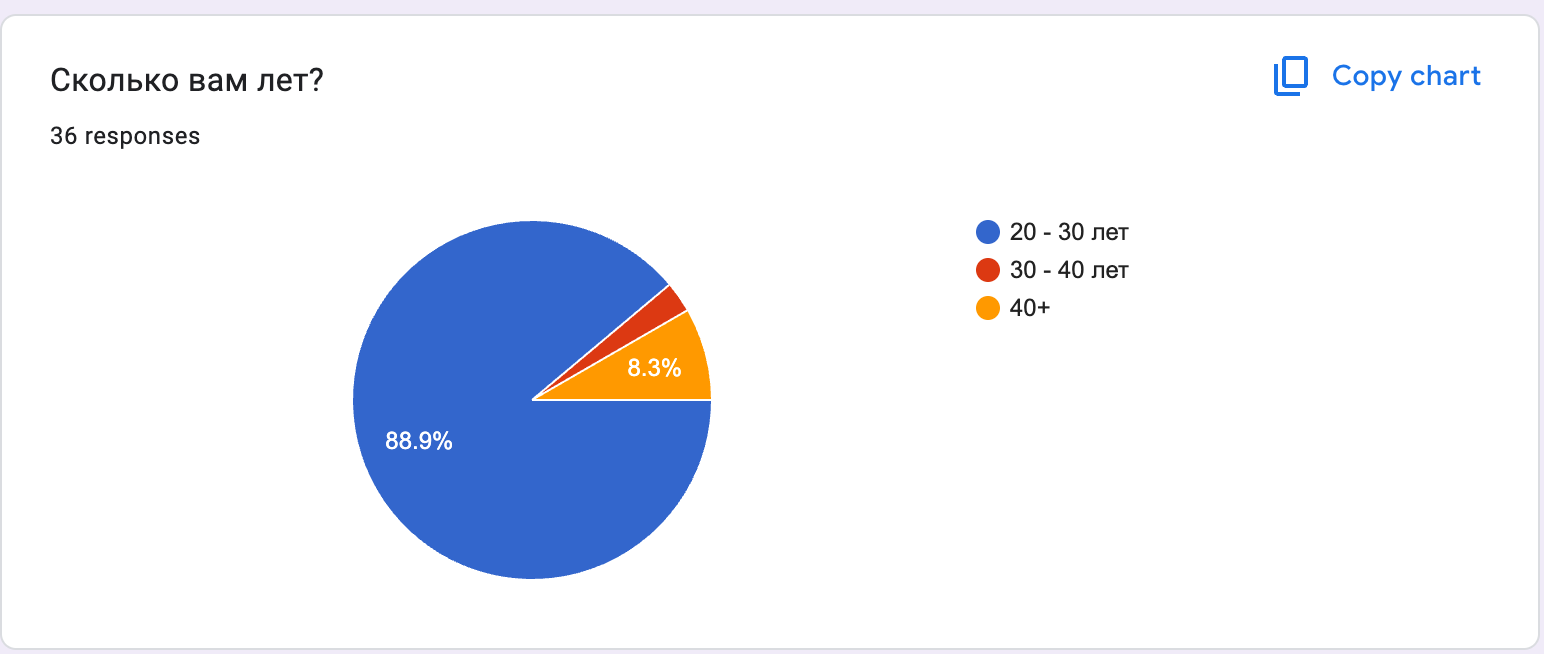
\includegraphics[width=0.7\linewidth]{images/pool/question_1.png}}
    \captionof{figure}{Результаты демографии}
    \label{fig:enter-label}
}

Касаемо профессии, больше половины принявших участие респондентов являются частными репетиторами. На 2 месте по частоте - преподаватели частных школ (рисунок 2).


\vspace{12pt}
{
    \centering
    \fbox{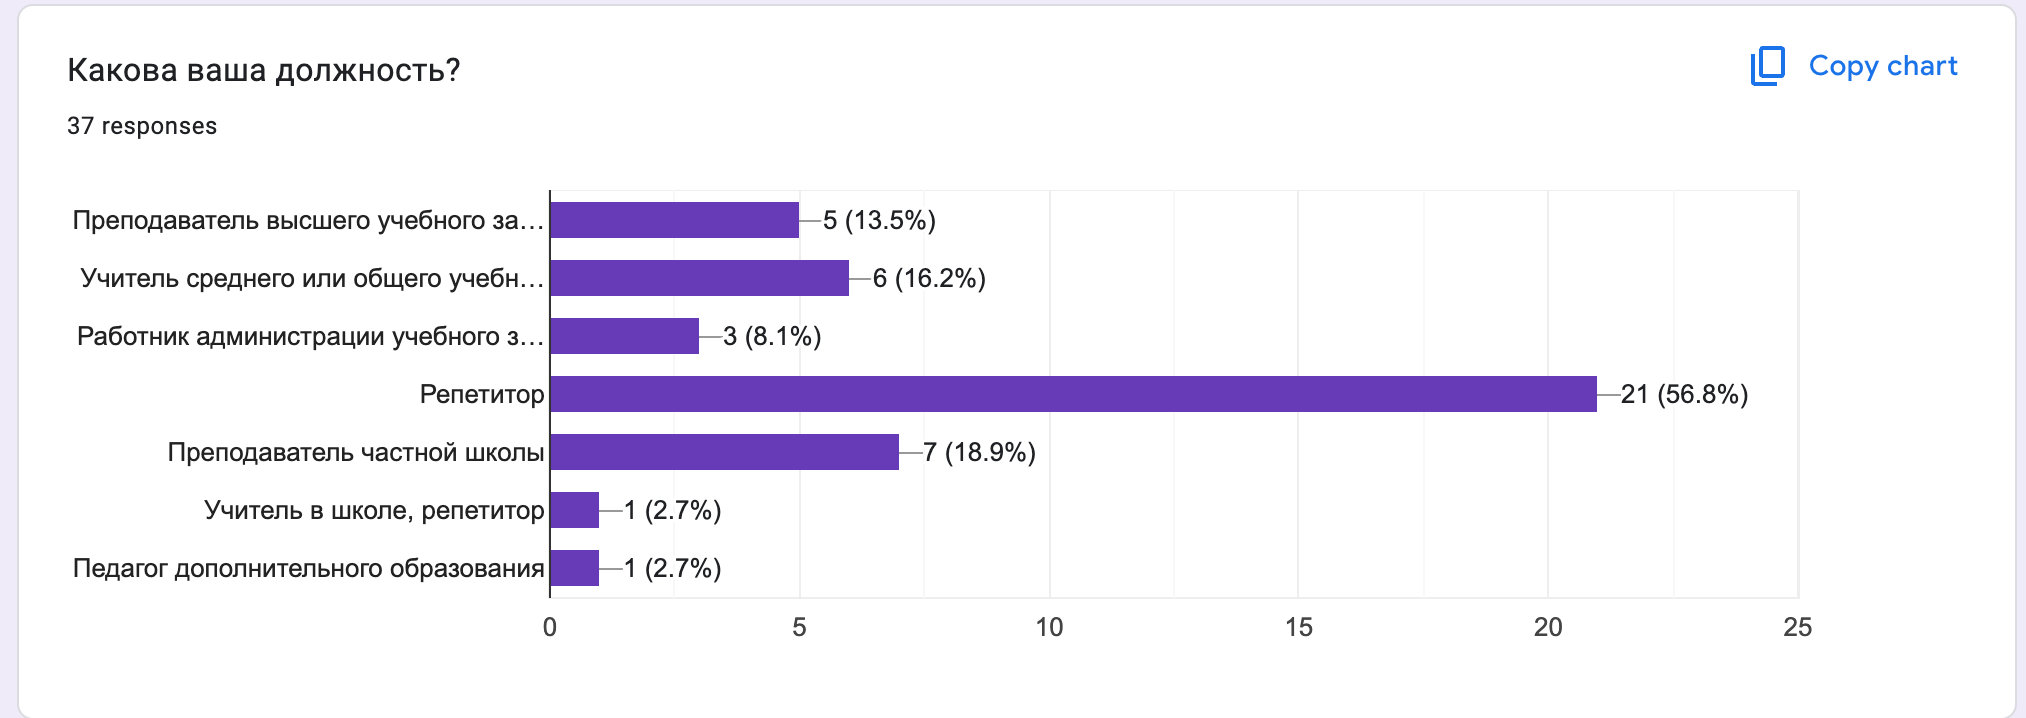
\includegraphics[width=0.8\linewidth]{images/pool/question_2.png}}
    \captionof{figure}{Статистика по профессии}
    \label{fig:enter-label}
}

Благодаря этой метрике, можно сегментировать ответы и определить в какой сфере относятся самые часто встречающиеся трудности. 

Далее, согласно вопросу об опыте в сфере образования (рисунок 3), 45.9\% опрошенных имеют опыт от 2 до 5 лет, 40.5\% только начинают свой путь в образовательной деятельности, и лишь 13\% опрошенных имеют более серьезный опыт.

\vspace{12pt}
{
    \centering
    \fbox{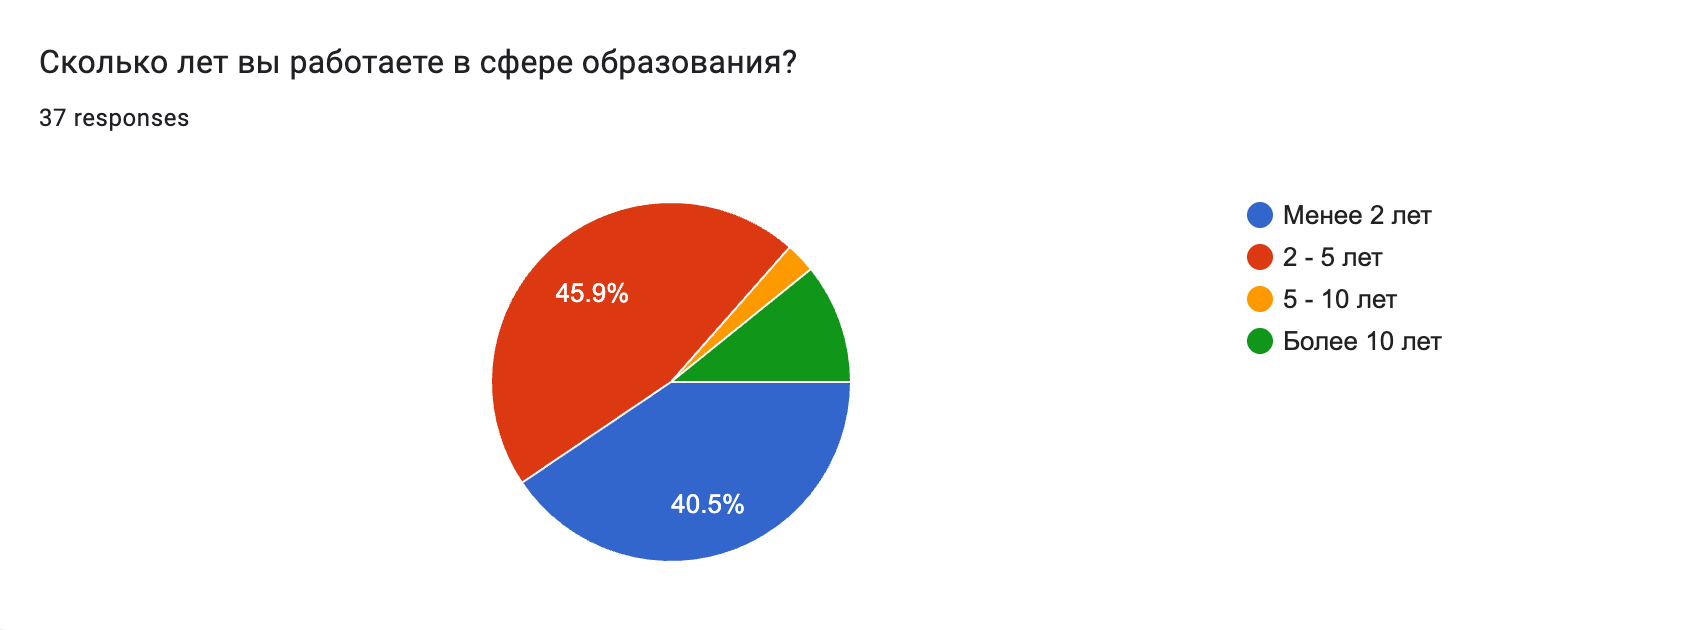
\includegraphics[width=0.8\linewidth]{images/pool/question_3.png}}
    \captionof{figure}{Опыт респондентов}
    \label{fig:enter-label}
}

Представленные показатели дают основание для более детального изучения факторов, влияющих на эффективность педагогической деятельности. Сравнительный анализ временных затрат различных категорий педагогов открывает новые перспективы для оптимизации рабочего процесса.

Следующий вопрос был направлен на выяснение самых времязатратных задач в работе респондентов (рисунок 4).

\vspace{12pt}
{
    \centering
    \fbox{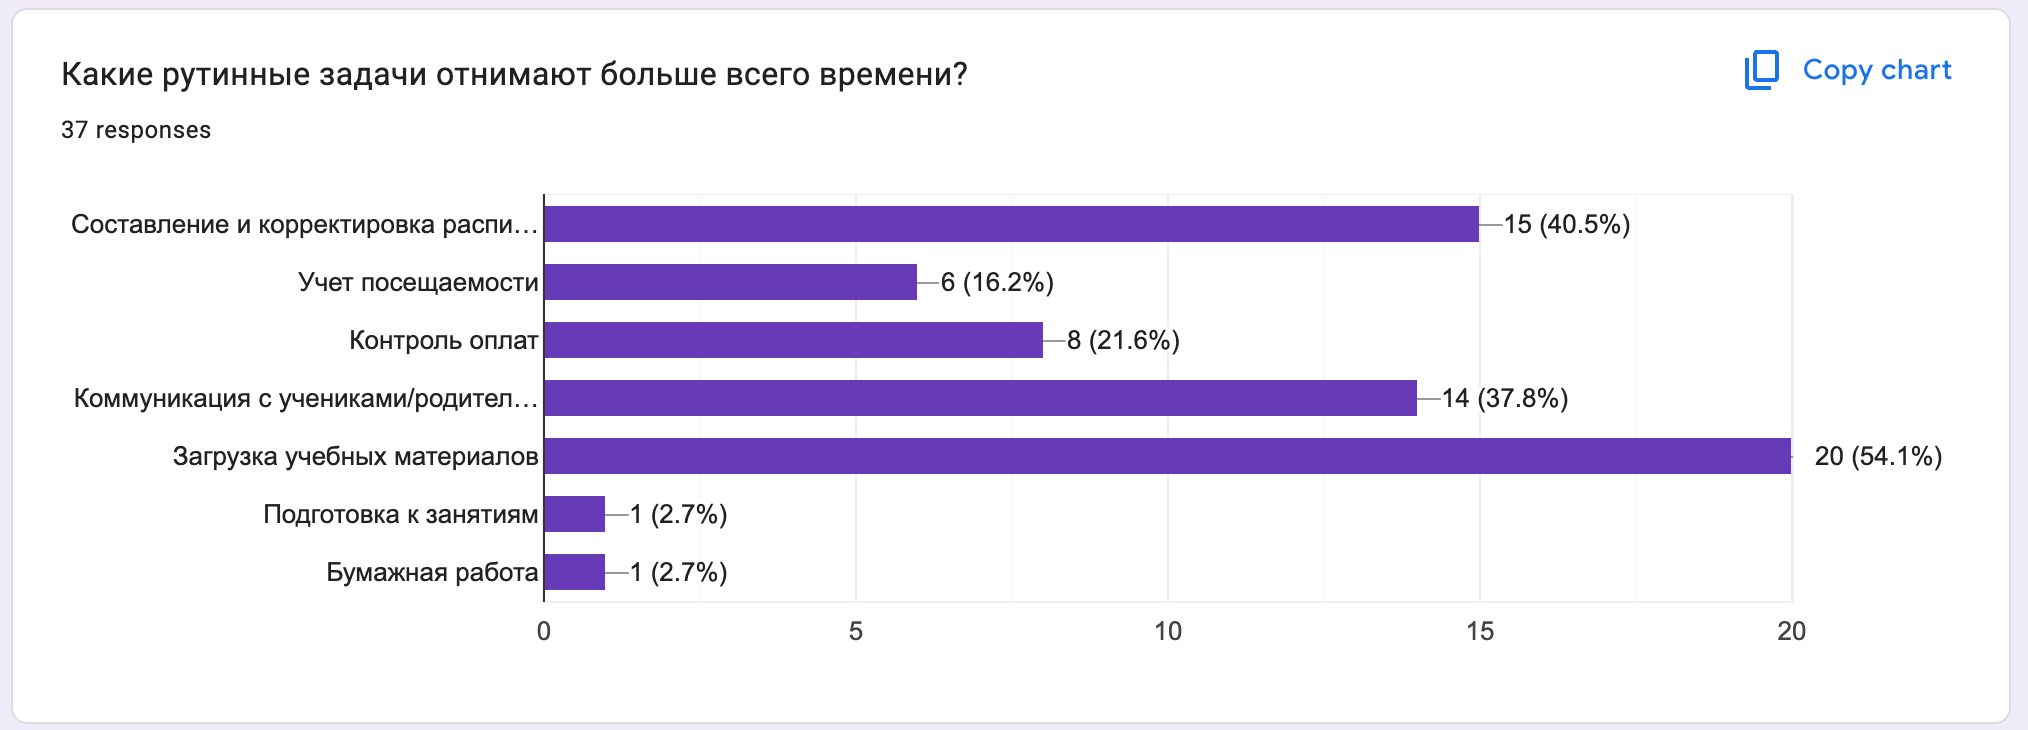
\includegraphics[width=0.7\linewidth]{images/pool/question_4.png}}
    \captionof{figure}{Самые времязатратные задачи}
    \label{fig:enter-label}
}

Из рисунка 4 можно сделать вывод о том, что самой времязатратной задачей являетсяя загрузка учебных материалов, составление и корректировка расписания и коммуникация с учениками. 

Также из общей таблицы ответом можно получить ифномацию о том, что с проблемой загрузки учебных материалов сталкиваются в основном репетиторы, когда с проблемой коммуникации сталкиваются в основном учителя среднего образования, а учет посещаемости является главной проблемой преподавателей частных школ. Это говорит о том, что эти процессы требуют автоматизации.

На рисунке 5 представлены результаты вопроса, направленного на выявление инструментария, которым пользуются респонденты сейчас для решения своих повседневных задач. 

\vspace{12pt}
{
    \centering
    \fbox{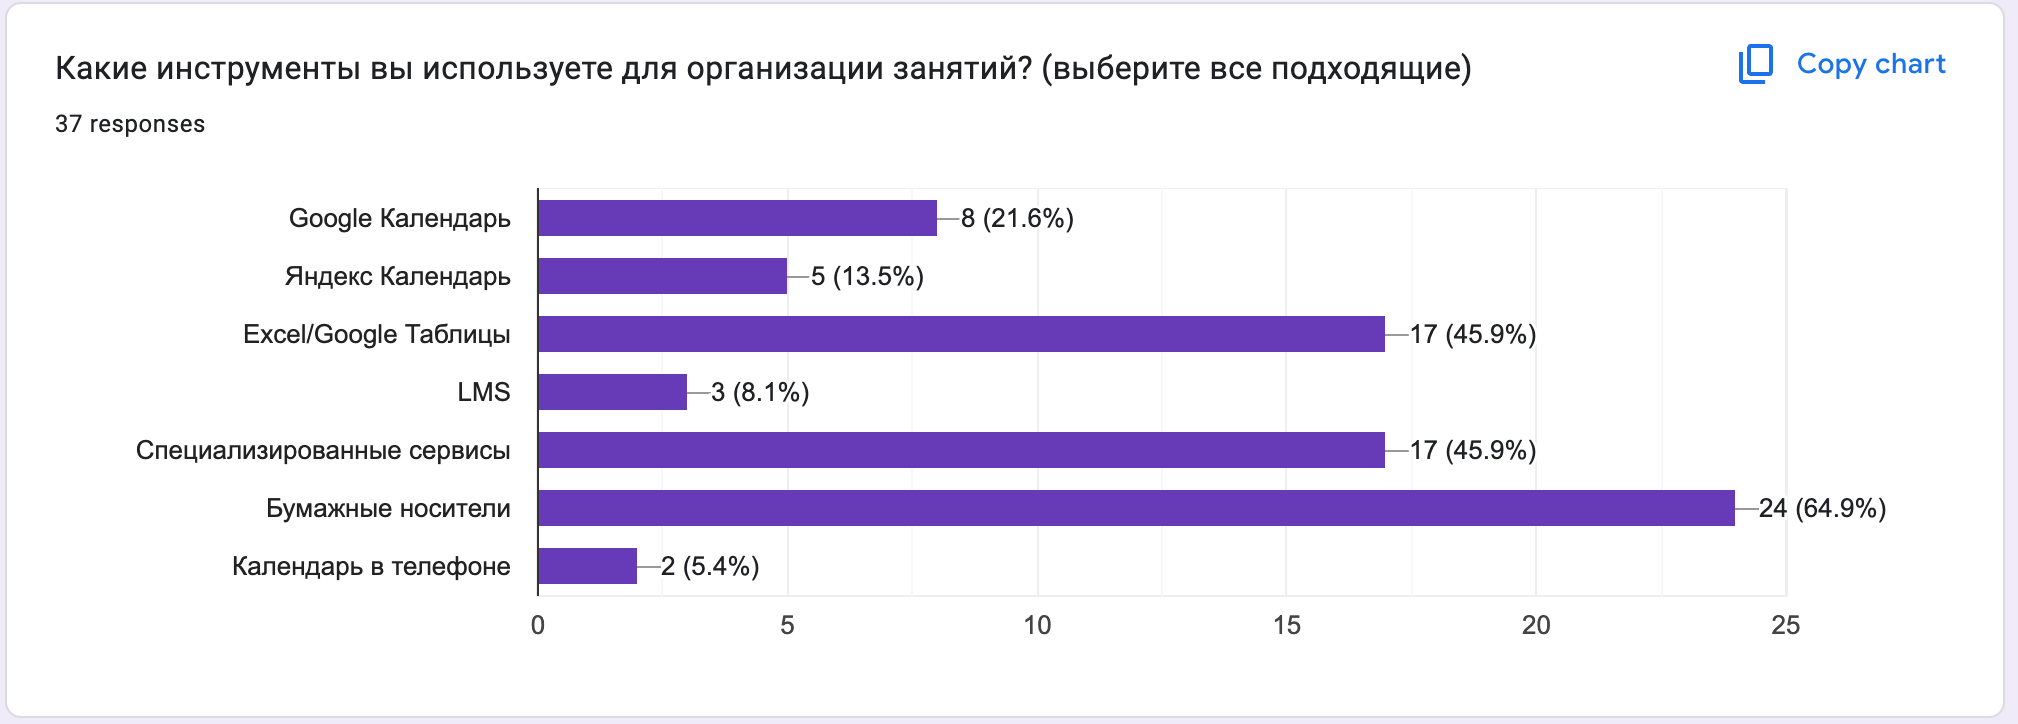
\includegraphics[width=0.8\linewidth]{images/pool/question_5.png}}
    \captionof{figure}{Наиболее используемые инструменты}
    \label{fig:enter-label}
}

Из ответов видно, что 64\% опрошенных предпочитают вести учет своей деятельности на бумаге и лишь 35\% предпочитают использовать электронные носители. Это дает сигнал о том, что многие респонденты не готовы использовать специализированные сервисы, поскольку, эти же респонденты, что выбрали основной инструмент - бумагу, ответили, что главной их проблемой является дублирование и потеря информации. Исходя из этого можно сделать вывод о том, что эта часть целевой аудитории желает перейти от традиционног ведения учета на бумаге к более подходящему решению и испытывает трудности.

Также, из рисунка 5 можно сделать простой вывод о том, что хоть 45\% ответили, что используют специлизированные сервисы, также используют Excel. Это говорит о фрагментации данных. Респонденты вынуждены использовать множество сервисов одновременно и это подтверждает нишу предлагаемого решения.

На рисунке 6 представлен вопрос о владения компьютером. 

\vspace{12pt}
{
    \centering
    \fbox{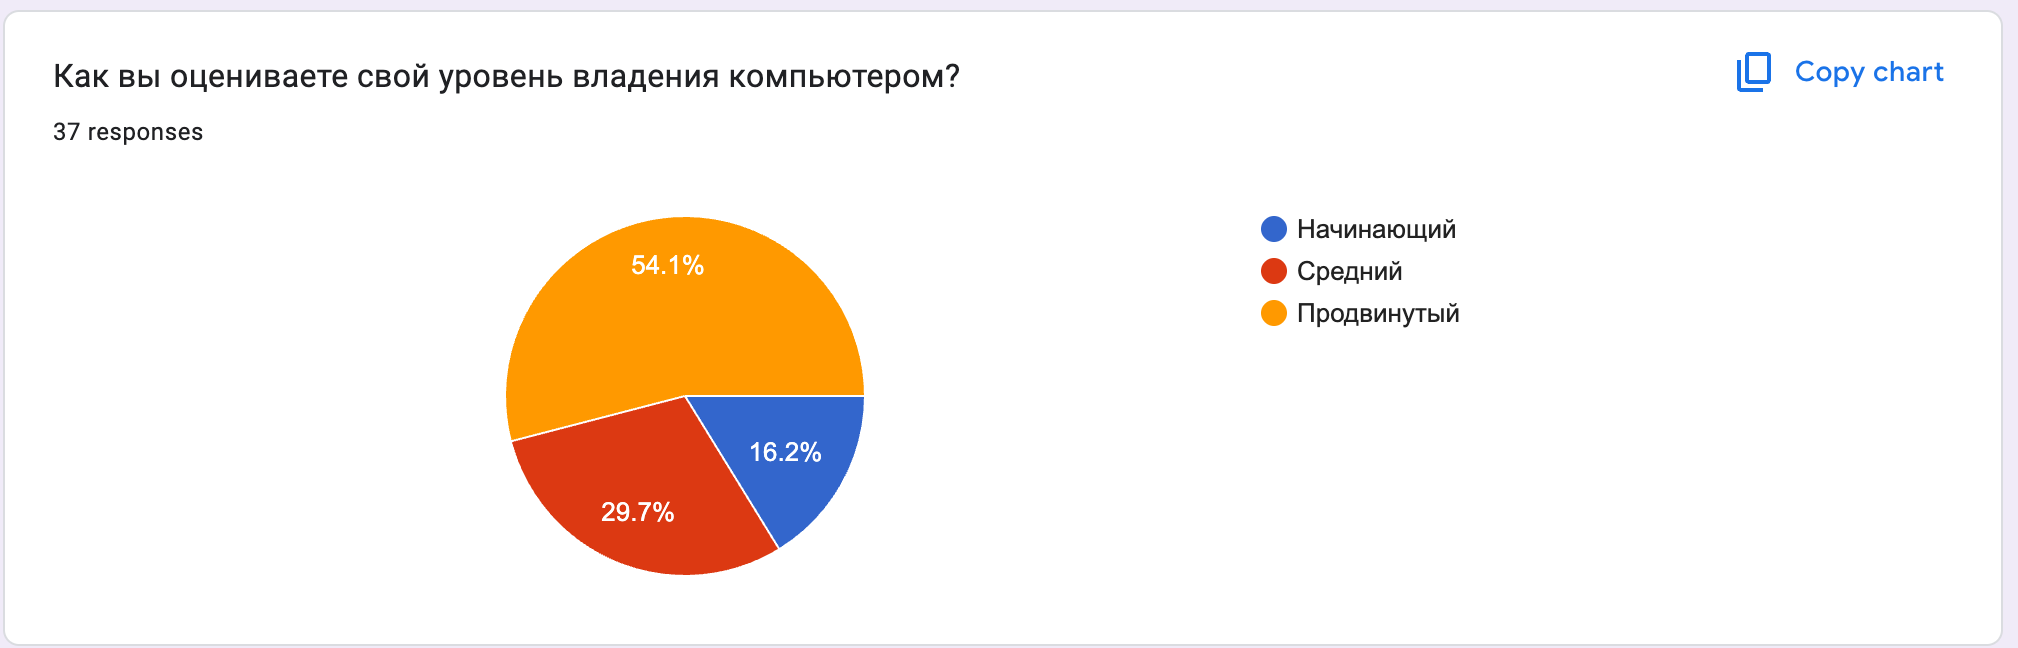
\includegraphics[width=1\linewidth]{images/pool/question_6.png}}
    \captionof{figure}{Уровень владения компьютером}
    \label{fig:enter-label}
}

Из результатов вопроса можно сделать уверенный вывод о том, что большая часть целевой аудитории имеет высокий или же средний уровень владения персонального компьютера. Это значит, что внешний вид и интерфейс веб-приложения должен быть простым, интутивно понятным и не вызывать большой когнитивной нагрузки. Он должен соответствовать базовым правилам читаемости текста на экранах.

Вопрос 7 (рисунок 7) нацелен на выявление уровней удовлетворенности и неудовлетворенности целевой аудитории с сервисами, которые они привыкли использовать сейчас.

\vspace{12pt}
{
    \centering
    \fbox{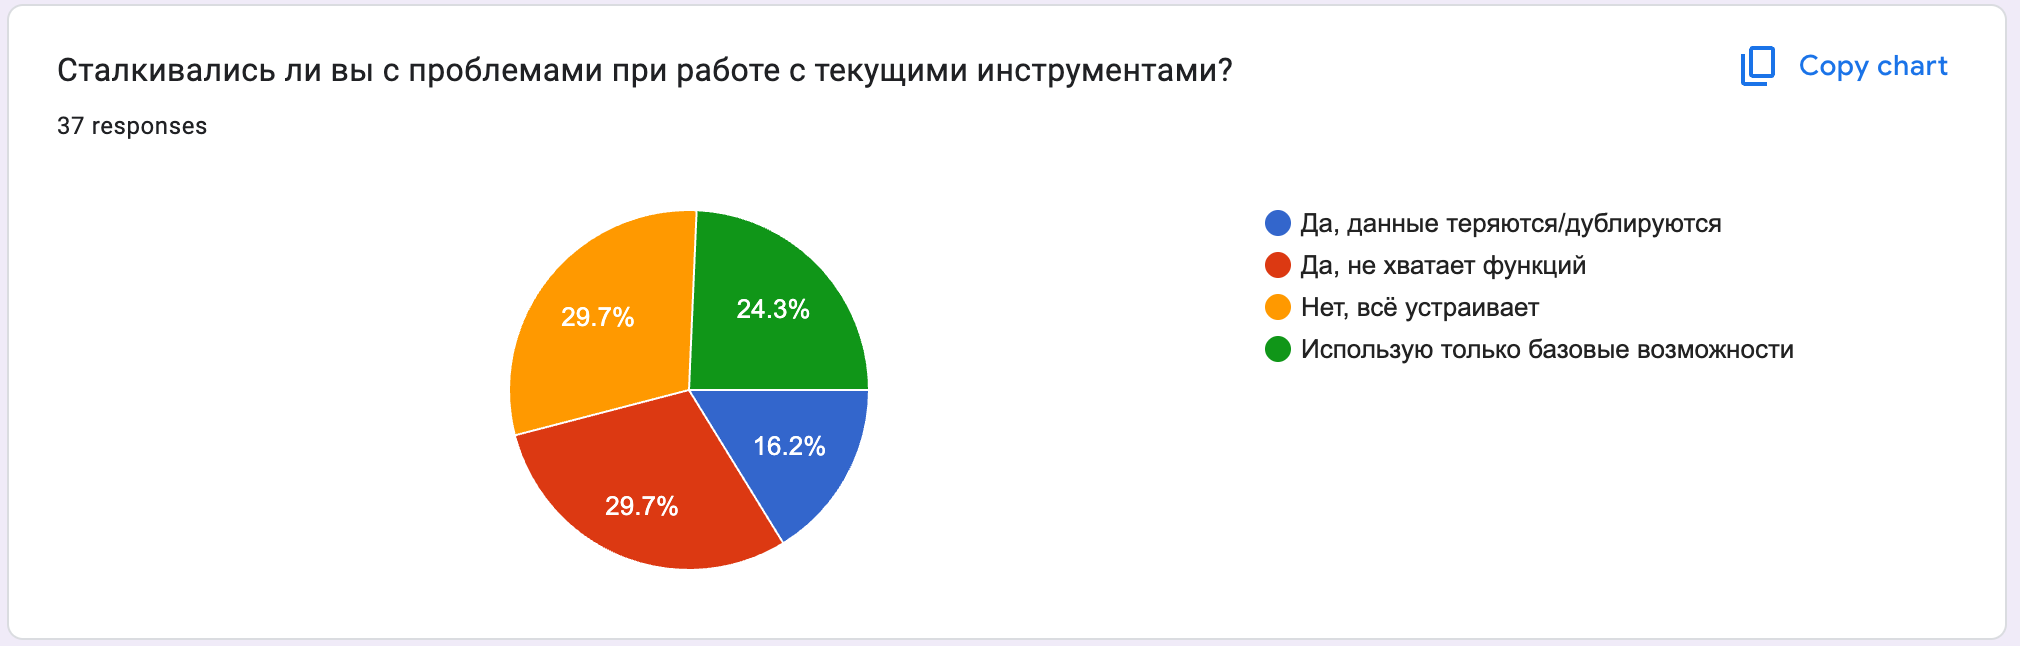
\includegraphics[width=0.9\linewidth]{images/pool/qustion_7.png}}
    \captionof{figure}{Удовлетворенность текущими решениями}
    \label{fig:enter-label}
}

Здесь видно, что мнения респондентов разделились. Около трети респондентов ответили, что им не хватает некоторого функционала, 16\% заявлили им не хватает критически важного функционала и испытывают проблемы с хранением информации. Это дает основание полагать, что предлагаемое решение будет особенно актуально для минимизирования ручного труда.

По итогам 8 вопроса, представленного на рисунке 8, можно сделать вывод о том, что весь перечисленный функционал востребован среди целевой аудитории.

\vspace{12pt}
{
    \centering
    \fbox{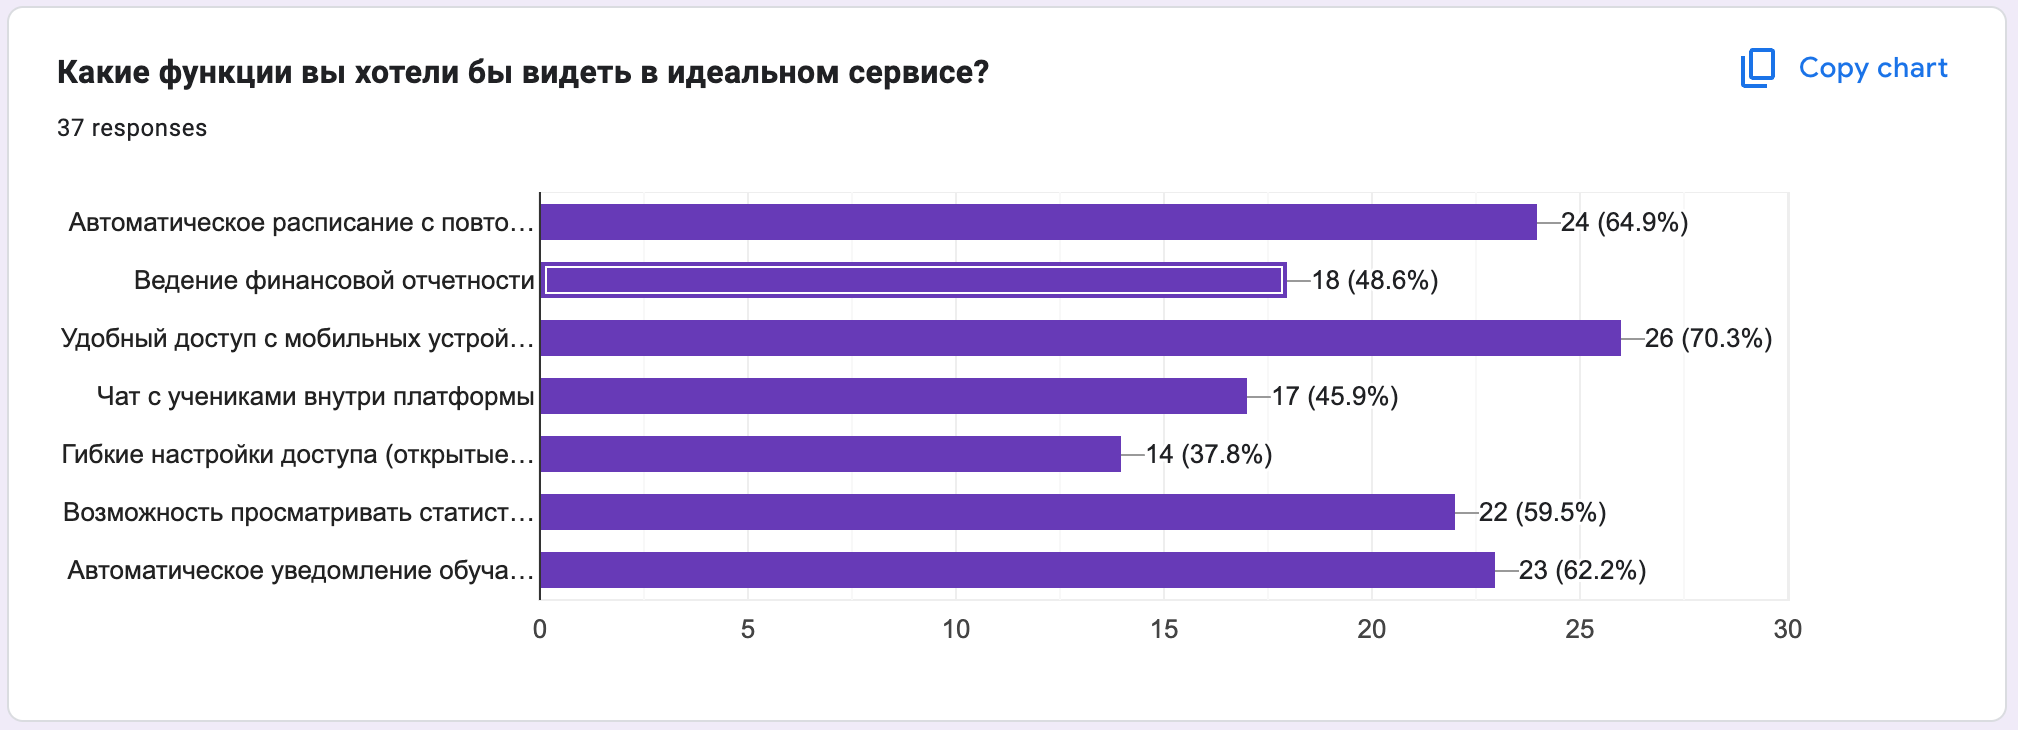
\includegraphics[width=0.9\linewidth]{images/pool/question_8.png}}
    \captionof{figure}{Функции идеального сервиса}
    \label{fig:enter-label}
}

Из сводной таблицы, можно сделать вывод о том, что те респонденты, которые указали своей главной проблемой «Составление и корректировка расписания», использующие Excel больше всего выбрали желаемый функционал «Автоматическое расписание с повторяемыми занятиями», а также «Ведение финансовой отчетности». 

Также, те респонденты, чей уровень владения компьютером явлется начинающим или средним, заявили о своей потребности в сущестовании адаптированной версии веб приложения под мобильные устройства, такие как телефон, планшет и небольшие компьютеры.

А гибкие настройки доступа, разделение групп обучающихся на открытые и закрытые, отметили в основном репетиторы и преподаватели частных школ и заведений.

Из результатов проведенного опроса, можно составить портрет среднестистического пользователя системы администирования групповых занятий. 
 
Портрет ЦА:

\begin{enumerate}
    \item Возраст: 25–35 лет.
    \item Опыт работы: 2-10 лет.
    \item Техническая подготовка: средний уровень.
Многие не имеют опыта работы с профессиональными CRM или LMS, но активно используют базовые инструменты (Яндекс Календарь, Excel, мессенджеры).
\end{enumerate}

Потребности:

\begin{enumerate}
    \item Быстрое создание групп и расписаний без ручного ввода данных.
    \item Учет посещаемости с возможностью отметки в реальном времени.
    \item Автоматический расчет доходов.
    \item Доступ к статистике (посещаемость, оплаты, успеваемость).
\end{enumerate}

Проблемы, с которыми сталкиваются:

\begin{enumerate}
    \item Фрагментация инструментов: расписание в одном месте, оплаты в другом, общение в мессенджере.
    \item Сложности с контролем задолженностей учеников.
    \item Отсутствие единого пространства для работы с группами.
    \item Недостаток коммуникации с обучающимися.
\end{enumerate}

Также, для автоматизации процесса ведения груп, а также расширения функциональности системы, проанализирована вторичная аудитория: обучающиеся.

Портрет ЦА:

\begin{enumerate}
    \item Возраст обучающихся: 12–25 лет.
    \item Техническая подготовка: средняя. Хорошо владеют компьютером и телефоном, но не имеют навыков работы в профессиональных CRM системах и LMS.
\end{enumerate}

Исходя из ответов респондентов, представленные в ответах на вопросы, а также использовав портрет целевой аудитории, можно определить основные потребности основной целевой аудитории.

Потребности:

\begin{enumerate}[label=\arabic*)]
    \item просмотр расписания занятий и домашних заданий;
    \item запись на групповые или индивидуальные занятия;
    \item доступ к истории оплат и посещаемости.
\end{enumerate}

Проблемы, с которыми сталкиваются:

\begin{enumerate}[label=\arabic*)]
    \item необходимость уточнять расписание у преподавателя;
    \item отсутствие прозрачности в оплатах.
\end{enumerate}

По сформированным портретам основной целевой аудитории можно определиться с списоком функциональных и нефункциональных требований к системе, которые будут нацелены на улучшение пользовательского опыта и решение главных задач целевой аудитории.


\section{Анализ аналогов и конкурентов}

Анализ аналогов – это процесс изучения существующих решений (конкурентов, продуктов, сервисов) с целью выявления их сильных и слабых сторон, функционала, ценовой политики и пользовательского опыта [5].

Анализ аналогов поможет понять, какие функции и подходы наиболее востребованы пользователями, а также выявить слабые стороны существующих решений. 

К сожалению, сегодня большинство преподавателей и репетиторов предпочитают использовать excel таблицы.

Преимущества:

\begin{enumerate}
    \item Приемственность. Многие используют Excel поскольку десятилетиями использовали его для выполнения всех своих рутинных задач и попросту не хотят переходить на что-то более новое.
    \item Доступность. Excel предустановлен по умолчанию на всех Windows устройствах и доступен сразу «из коробки». Пользователю сразу доступен весь основной функционал приложения без необходимости устанавливать дополнительное ПО самому.
    \item Удобство хранения. Некоторые xslx редакторы поддерживают облачное хранение, обеспечивая своим пользователем общий доступ с разных устройств, лишая их необходимости в ношении своего устройства накопления информации на постоянной основе.
\end{enumerate}

Недостатки:

\begin{enumerate}
    \item Сбор информации. Пользователю необхожимо вручную вводить информацию по каждому своему ученику на каждое занятие. На это тратится много времени, а также много теряется на построение коммуникации вне системы.
    \item Отсутствие целевой направленности. Изначально excel не строился как платформа для исследуемой целевой аудитории, а следственно не может учитывать их потребности.
    \item Переполненость функционалом. Excel редактор представляет собой многофункциональное приложение, способности которого только затрудняют навигацию по приложению, отвлекая тем функционалом, который не требуется для достижения целей ЦА.
\end{enumerate}


Из опроса, был выявлен неочевидный, но распространенный инструмент - бумажный носитель.

Преимущества:

\begin{enumerate}
    \item Доступность. Блокнот или ежедневник, как правило, всегда под рукой у преподавателя.
    \item Простота использования. Поскольку писать могут абсолютно все, вести учет и заметки можно в любом виде.
\end{enumerate}

Недостатки:

\begin{enumerate}
    \item Ненадежность. Бумага - материал легко воспламенимый и подвержен влаге. Его крайне легко испортить, а значит быстро утратить важную ифнормацию.
    \item Времязатратность. Ведение ежедневника обязывает тратить значительное время на орагнизацию и структуризацию данных. Это является главным недостатком, поскольку это время сегодня - главный ресурс.
\end{enumerate}


Ярепетитор - прямой конкурент предлагаемому решению, который предоставляет общий функционал создания занятий, просмотра расписания, учета заработка и оплаченных часов [6].

Однако, эта платформа обладает главным недостатком - односторонность использования. Система предоставляет функционал только для преподавателя и совсем игнорирует потребности обучающихся, чья оринетированность занимает ключевую роль в проведении образовательной деятельности.

Преимущества:
\begin{enumerate}
    \item Наличие календаря и возможность вести расписание.
    \item Возможность вести статистику заработка.
    \item Многоплатформенность. Сервис доступен как в веб версии, так и android и IOS приложение.
    \item  Наличие файлаобменника. Сервис предоставляет возможность хранения заданий и материалов к занятиям.
    \item Интеграция с сторонними сервисами. Сервис поддержвает авторизацию черех Google и Apple аккаунты.
\end{enumerate}

Недостатки:
\begin{enumerate}
    \item Пользователю приходится вручную заносить каждого своего ученика в систему, а также всю информацию о нем.
    \item Пользователю приходится самому уведомлять своих учениках о переносе занятия.
    \item Ученики пользователя не имеют возможности получить общую информацию о курсах и занятиях преподавателя без предварительной коммуникации. 
\end{enumerate}

Это пораждает лишнее потраченное время на согласование времени, цены и условия проведения занятий. 

Также, ЯРепетитор выделяет сложный и неинтуитивный интерфейс, затрудняющий использования расписания и создание занятий (рисунок 9).

\vspace{12pt}
{
    \centering
    \fbox{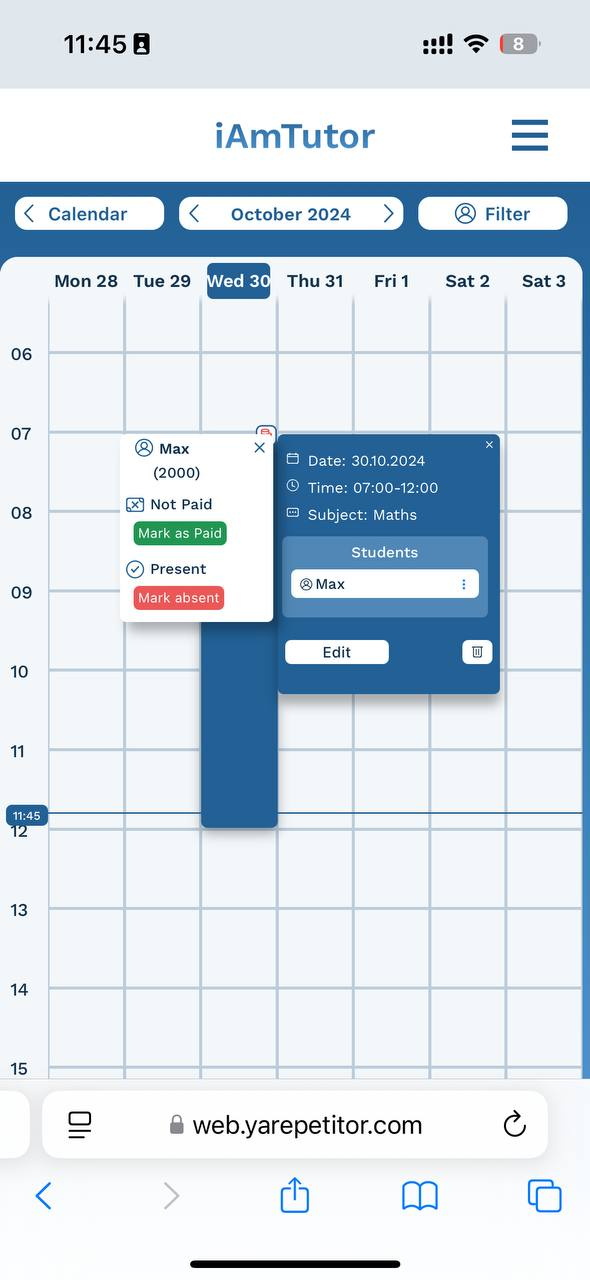
\includegraphics[width=0.9\linewidth]{analog1.jpg}}
    \captionof{figure}{Пример интерфейса аналога}
    \label{fig:enter-label}
}

Визуальные недостатки аналога:

\begin{enumerate}
    \item Проблемы с контрастностью и читаемостью. Слишком светлые или неконтрастные элементы интерфейса, например, серые кнопки или текст на белом фоне, что затрудняет восприятие информации, особенно для пользователей с ослабленным зрением.
   \item Неудобная навигация и организация контента. Сложная структура меню, из-за которой пользователи вынуждены совершать лишние действия для доступа к ключевым функциям (например, редактирование расписания через несколько шагов).
   \item Ошибки в отображении данных. Непоследовательное обновление интерфейса: пользователи отмечают, что после оплаты подписки или добавления учеников изменения не отражаются сразу, что вызывает путаницу 2 (отзывы Nas7usha7, T3lfi).
   \item Использование устаревших UI-компонентов, которые выглядят нефункционально (например, плоские кнопки без теней или градиентов).
\end{enumerate}

Преимущества:

\begin{enumerate}
    \item Специализация на групповых занятиях. Инструменты заточены под нужды преподавателей: быстрое создание групп, массовая отметка посещаемости.

    \item Все в одном месте. Объединение расписания, оплат, коммуникации и контента избавляет от необходимости переключаться между сервисами.

    \item  Простота для не технических пользователей. Минимум настроек, интуитивные формы, подсказки при первом входе.

    \item Финансовая прозрачность. Автоматические напоминания об оплате, статистика доходов/расходов.

\end{enumerate}



\section{Анализ требований}

Перед тем как приступить к проектированию системы, необходимо выявить все функицональные и нефункциональные требования, представленные к системе на основе опроса и конкурентов [7]. Полученные требования отражают фактический функционал и технические особенности системы. Они включают в себы сильные стороны используемых аналогов, а также стремятся исключить повторения недостатков конкурентов.

Общие функциональные требования представлены на UML диаграмме 
\hypertarget{pi10}{\hyperlink{pic10_text}{рисунке Б.1}}.

Рассмотрим функциональные требования для пользователей с ролью преподавателя:

\begin{enumerate}
    \item Создание групп с настройкой параметров (макс. количество учеников, стоимость занятий).
    \item Составление гибкого расписания: повторяющиеся и разовые занятия. Перенос занятий.
    \item Отметка посещаемости с возможностю добавления комменатриев.
    \item Возможность указать стоимость каждого занятия.
    \item Введение статистики по доходам.
    \item Управление контентом: добавление материалов к занятиям и домашнего задания.
    \item Уведомление учеников о переносах или отмены занятий.
\end{enumerate}

Для обучающихся:

\begin{enumerate}
    \item Личный кабинет с расписанием и историей посещений занятий.
    \item Вступление в группы преподавателей и просмотр открытых окон.
    \item Вомзожность поиска преподавателей.
\end{enumerate}

Далее рассмотрим нефункциональные требования:

\begin{enumerate}[label=\arabic*)]
    \item удобство интерфейса. Современные паттерны применения дизайна, а также адаптивность под мобильные устройства;
    \item безопасность. Надежное хранение персональных данных;
    \item производительность. Возможность посещения платформы более 1000 человек одновременно;
    \item подержкка внешних сервисов, таких как вход через Google или Yandex аккаунты.
\end{enumerate}


\section{Описание необходимого функционала}

Для проектирования бизнес процессов выбрана методология описания схем IDEF0 [8]. Эта нотация является самой оптимальной для проведения описательных работ создания линейных бизнес процессов, требующие всеобъемлещего описания компонентов, элементов управления, действий, а также входных и выходных параметров.

Бизнес процесс авторизации в системе представлен на рисунке 10.

\vspace{12pt}
{
    \centering
    \fbox{
\includegraphics[width=0.6\linewidth]{images/idef0/image.png}}
    \captionof{figure}{Общий бизнес процесс входа в систему в нотации IDEF0}
    \label{fig:enter-label}
}

Этот процесс декомпозируется на регистрацию и авторизацию на уровень декомпозиции 1 и представлен на рисунке 11.

\vspace{12pt}
{
    \centering
    \fbox{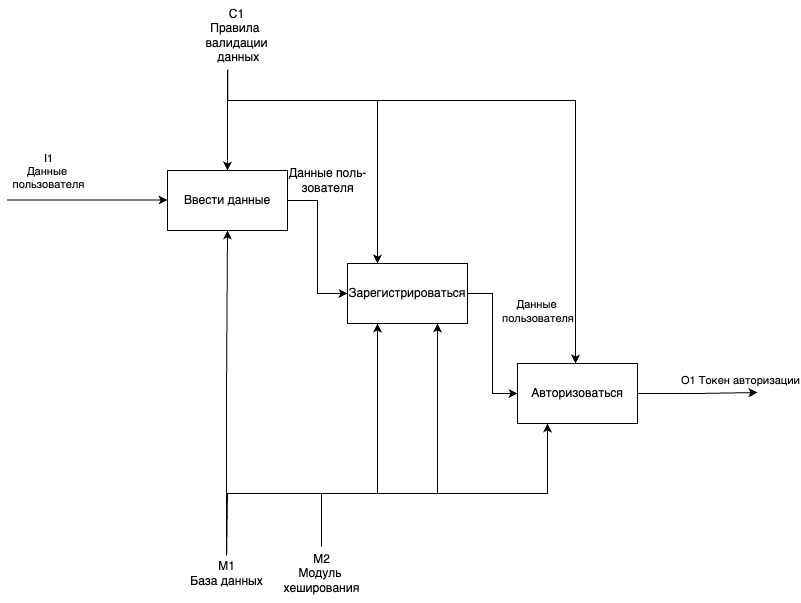
\includegraphics[width=0.7\linewidth]{images/idef0/image2.png}}
    \captionof{figure}{Процесс входа в систему в нотации IDEF0 на 1 уровне декомпозиции}
    \label{fig:enter-label}
}

Далее, рассмотрим процесс регистрации на рисунке 12. 

\vspace{12pt}
{
    \centering
    \fbox{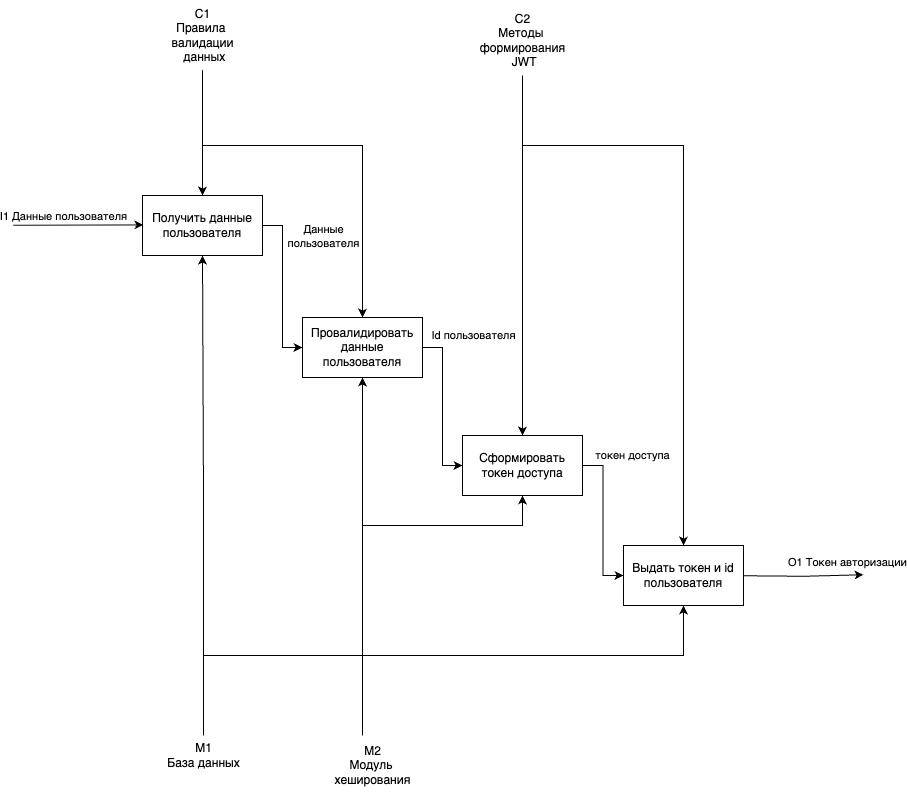
\includegraphics[width=0.65\linewidth]{images/idef0/image3.png}}
    \captionof{figure}{Процесс регистрации пользователя в нотации IDEF0}
    \label{fig:enter-label}
}

Здесь, на вход поступают данные пользователя, а на выход id нового пользователя. Из механизмов здесь принимает участие модуль хеширования паролей, а также база данных в которой хранятся данные. Из правил, здесь присутствует Правила валидации полей.


В процессе регистарции существует процесс валидации данных, декомпозированный на рисунке 13.

\vspace{12pt}
{
    \centering
   \fbox{ 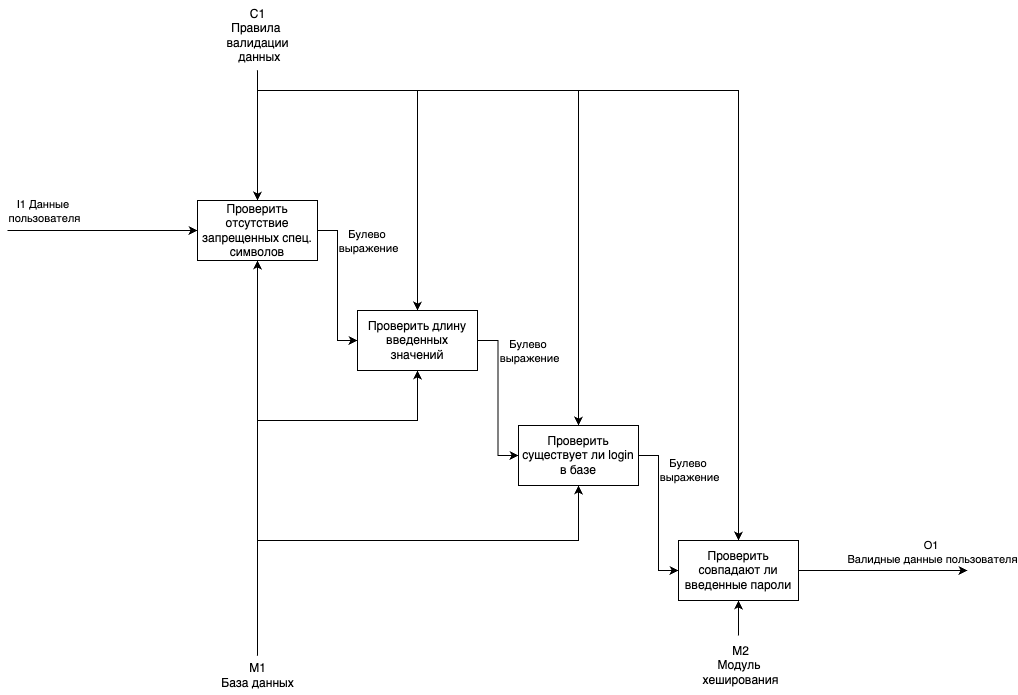
\includegraphics[width=0.8\linewidth]{images/idef0/image4.png}}
    \captionof{figure}{Процесс валидации данных в нотации IDEF0}
    \label{fig:enter-label}
}
Здесь данные сначала валидируется по типу данных (строки числа или другое), далее проверяется существование введенного логина в базе данных, а также сверяются введеные пароли. 

После того как пользователь зарегистрирован, ему необходимо авторизоваться под своим логином для доступа в систему. 

Доступ в систему ограничен специальным токеном авторизации, который пользователь получает по факту авторизации и имеет срок истечения. По истечению срока действия токена, пользователю необходимо заново авторизоваться.

В процессе авторизации, представленном на рисунке 14, также используется процесс валидации введенных данных, после чего формируется уникальный идентификатор доступа в систему.

\vspace{12pt}
 {
     \centering
     \fbox{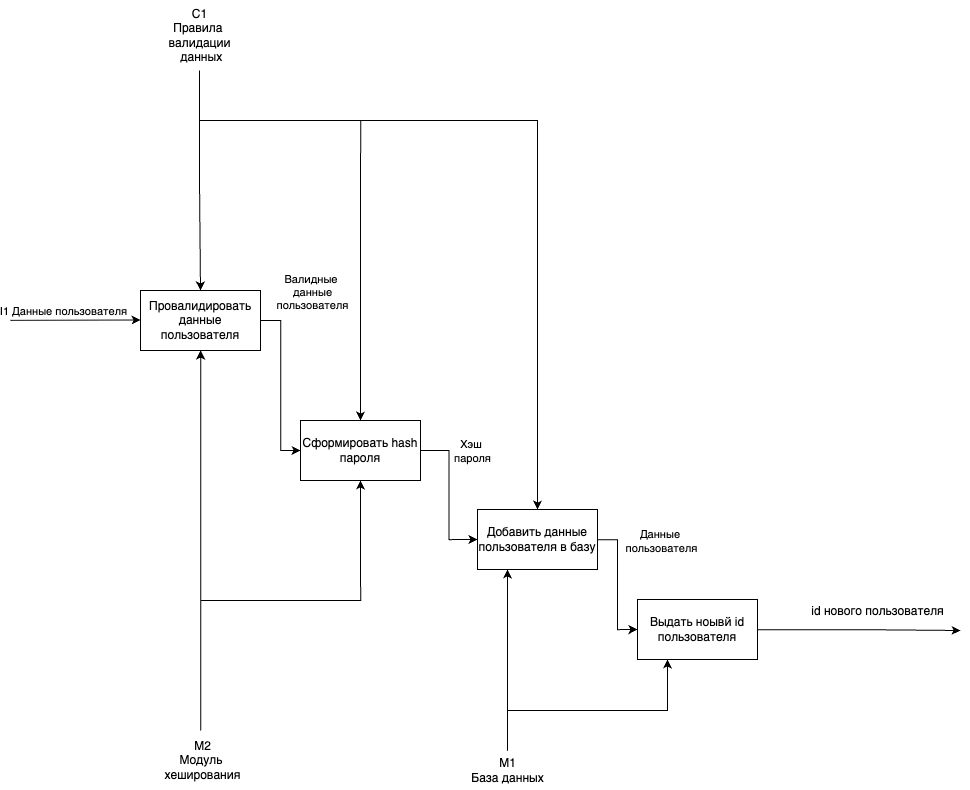
\includegraphics[width=0.5\linewidth]{images/idef0/image5.png}}
     \captionof{figure}{Процесс авторизации в нотации IDEF0}
     \label{fig:enter-label}
 }

Далее рассмотрим процесс вступления обучающихся в группы. Этот процесс представлен на рисунке 15 в виде диаграммы в нотации BPMN.

\vspace{12pt}
{
     \centering
     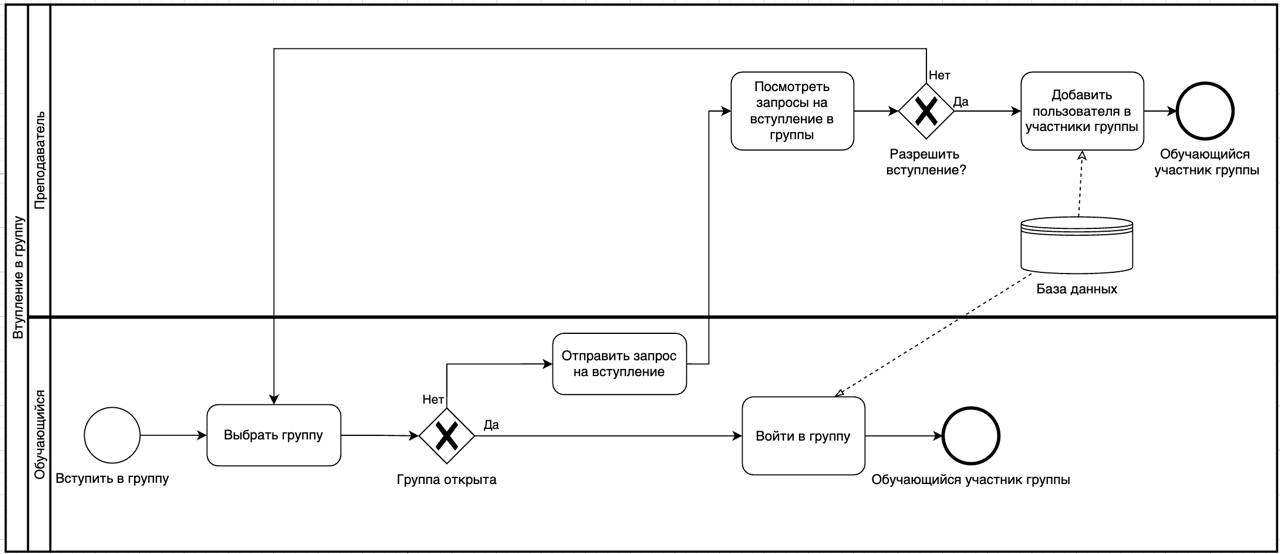
\includegraphics[width=0.8\linewidth]{images/bpmn_grpups.jpg}
     \captionof{figure}{Процесс вступления в группу в нотации BPMN}
     \label{fig:enter-label}
 }

 Здесь, пользователь, сначала выбирает желаемую группу из списка доступных групп. В случае если группа открыта, то у пользователя есть прямая возможность стать её участником. Этот процесс сопрвождается добавлением новой записи в таблицу участников групп.

 В случае если группа закрыта, создается запрос на вступление в выбранную группу. Создатель этой группы может просмотреть этот запрос, принять участника в группу или нет. Если да, пользователь также добавляется в таблицу участников группы, иначе запрос отклоняется, пользователю предложено выбрать новую группу.

 При этом сам запрос администратор группы не может удалить. Его может удалить только отправитель запроса, в случае если он отзовет заявку на вступление в группу. Администратор также может передумать и спустя время принять заявку на вступление и впустить участника. 

 После вступления пользователя в группу, у ученика в расписании должны отображаться все действующие занятия, проводимые в группе. Раписание предусматривает отображение в виде текущего дня, выбранного дня, недельного представления, а также месячного представления.

 В расписании, ученик может перейти в него и посмотреть актуальную ифнормацию о предстоящем занятии.

 Создатель занятия, он же создатель группы, может управлять текущими участниками занятия. Устанавливать присутсвие или отсуствие, указать была ли проведена оплата, а также имеет возможность в таблице добавть свои уникальные столбцы для каждого занятия, в которых он может указывать необходимую ему информацию. Например, это могут быть некие оценки - успеваемость по предметам, или учитывать комментарии по каждому участнику.


 \section{Выводы по аналитической части}

 В результате проведения аналитической работы были выполнены следующие задачи:
 \begin{enumerate}
     \item Проанализирована предметная область.
     \item Получен портрет целевой аудитории.
     \item Рассмотрены аналоги и составлены требования к системе.
     \item Описаны функциональные бизнес процессы.
 \end{enumerate}


\newpage
\chapter{ПРОЕКТНАЯ ЧАСТЬ}

\section{Анализ техническийх требований}

Для реализации функциональных и нефункциональных требований, необходимо определиться с актуальным списком технологий. Поскольку итоговым продуктом является веб-приложение, то согласно статье [9], современное веб приложение имеет следующие ключевые особенности в разработке:
\begin{enumerate}

\item Отличие в отображении. В отличие от традиционных приложений, веб-приложения функционируют в браузере и предоставляют пользователю взаимодействие с контентом на веб-страницах. Это связано с тем, что веб-приложения базируются на веб-технологиях, таких как HTML [10], CSS [11] и JavaScript [12], которые позволяют создавать интерактивные интерфейсы и обеспечивать гибкость в работе с различными устройствами.

\item Раздление компонентов. Веб-приложение как правило состоит из трех основных компонентов: клиентской стороны, серверной стороны и базы данных. Клиентская сторона отвечает за отображение инфорации пользователю и взаимодействие с ним, серверная сторона обрабатывает запросы клиента и принимает решения на основе логики приложения, а база данных хранит и обрабатывает данные, необходимые для работы приложения.

\item Особенности работы. Веб-приложения работают в режиме клиент-серверной архитектуры. Когда пользователь отправляет запрос, браузер обращается к серверу, который обрабатывает запрос и отправляет обратно отображаемые данные. Для этой цели используется протокол HTTP [13], который обеспечивает передачу данных между браузером и сервером. Таким образом, веб-приложения работают через сеть и доступны пользователю в любом месте, где есть доступ к интернету.
\end{enumerate}

% Далее в пунктах 2.2 - 2.7 будут рассмотрены аспекты структуры базы данных, отдельные классы реализации бизнес логики взаимодействия с базой данных, результаты разработки внешнего вида интерфейса, а также аспекты разработки клиентской части приложения.

\section{Проектирование базы данных}

В качестве системы управления базой данных было выбрано PostreSQL [14]. PostgreSQL - открытая российская система управления базами данных. Она базируется на языке SQL и поддерживает многие из возможностей стандарта SQL:2011 и ряд возможностей SQL:2016 в части работы с данными в формате JSON [15].

Сильными сторонами [16] PostgreSQL являются:
\begin{enumerate}[label=\arabic*)]
    \item высокопроизводительные механизмы транзакций и репликации;
    \item расширяемая система встроенных языков программирования: в стандартной поставке поддерживаются PL/pgSQL, PL/Perl, PL/Python и PL/Tcl, а также имеется поддержка загрузки модулей расширения на языке C;
    \item наследование;
    \item встроенная поддержка слабоструктурированных данных в формате JSON с возможностью их индексации;
    \item расширяемость (возможность создавать новые типы данных, типы индексов, языки программирования, модули расширения, подключать любые внешние источники данных).
\end{enumerate}

В PostgreSQL есть следующие ограничения:
\begin{enumerate}[label=\arabic*)]
    \item максимальный размер таблицы: 32 Тбайт;
    \item максимальный размер поля: 1 Гбайт;
    \item максимум полей в записи: 250—1600.
\end{enumerate}

На рисунке 16 представлена общая даталогическая модель базы данных. Она включает в себя 11 таблиц и описывает связи между ними.

\vspace{12pt}
{
    \centering
    \fbox{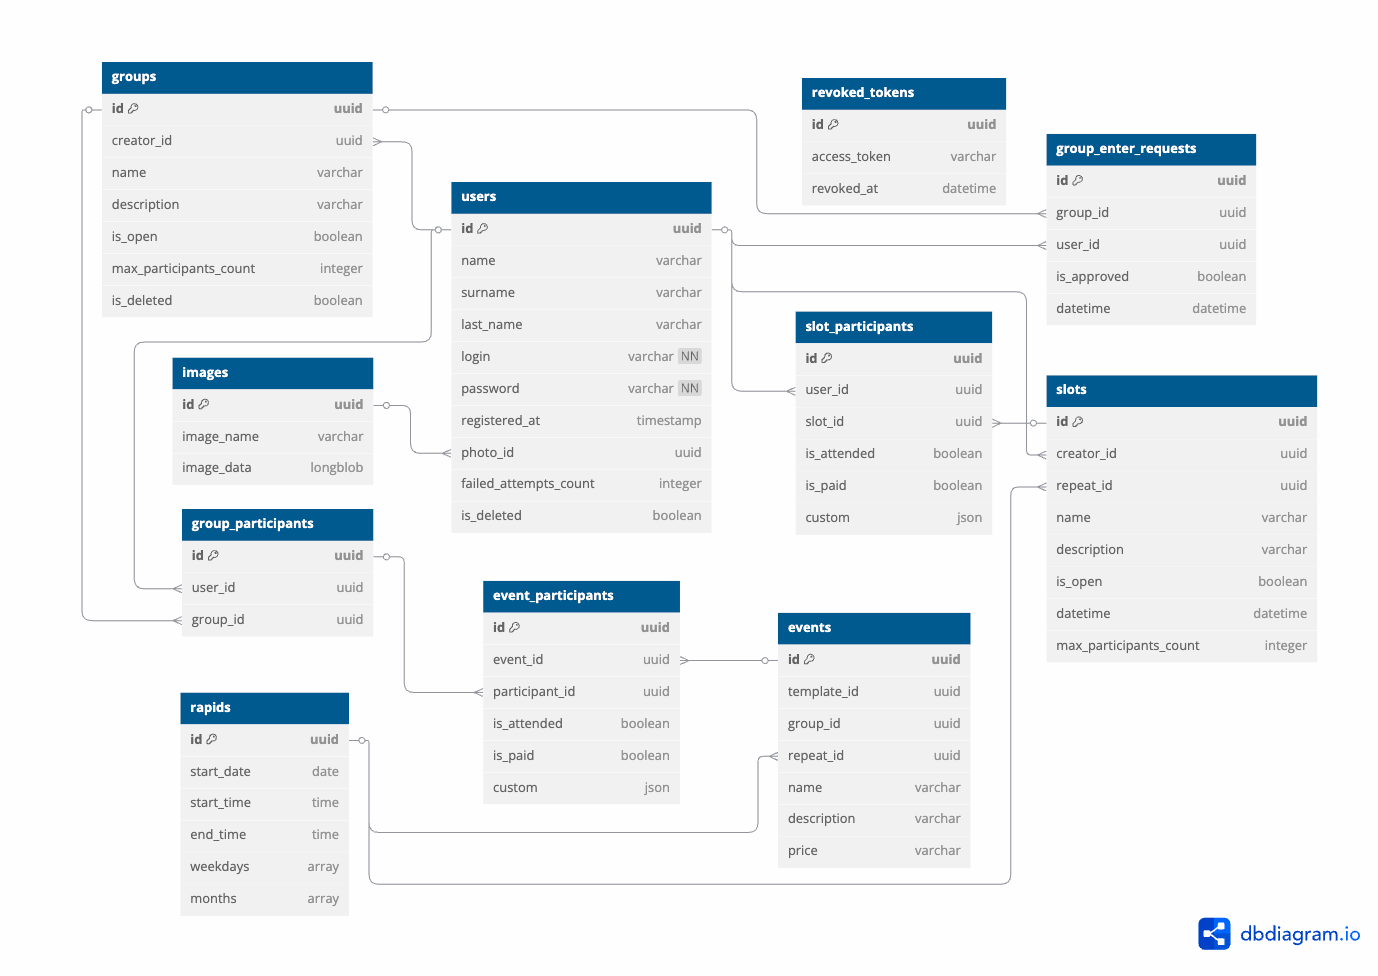
\includegraphics[width=0.95\linewidth,
          decodearray={0.0 1.0 0.0 1.0 0.0 1.0}]{images/DataBase.png}}
    \captionof{figure}{Схема реляционной базы данных}
    \label{fig:enter-label}
}

Таблица о пользователях users. Содержит информацию о зарегистрированных пользователях в системе.

Основные поля таблицы:

\begin{enumerate}[label=\arabic*)]
    \item login - уникальный логин авторизованного пользователя;
    \item password - хешированный пароль;
    \item photo\_id - идентификатор фотографии;
    \item role\_name - имя роли.
\end{enumerate}

Здесь поле photo\_id является связью один к одному, поскольку у одного пользователя может быть одно изображение, и ни у кого другого пользователя быть не может. Информация об изображениях хранится в таблице images.


Таблица images. Содержит информацию об изображениях пользователей.

Основные поля таблицы:

\begin{enumerate}[label=\arabic*)]
    \item image\_name - название файла;
    \item image\_data - base64 формат картинки.
\end{enumerate}



Таблица groups. Содержит информацию о группах - объединения пользователей по общему признаку. 

Существуют группы открытые как для всех пользователей, так и с ограниченным доступом, за это отвечает поле is\_open.

Все пользователи группы должны присутствовать на всех занятиях, которые создаются управляющим группы.

В открытые могут вступать абсолютно все пользователи, если количество участников группы меньше чем значение поля max\_participants\_count. 

В закрытые можно вступить, отправив запрос на вступление, который рассмотрит создатель группы.

Основные поля таблицы:

\begin{enumerate}[label=\arabic*)]
    \item name - название группы;
    \item max\_participants\_count - максимальное количество участников;
    \item description - описание;
    \item is\_open - флаг об открытости группы;
    \item creator\_id - id пользователя, который создал группу.
\end{enumerate}

Пример SQL запроса на получение всех открытых групп, представлен на листинге 2.1.

\begin{lstlisting}[language=SQL, caption=Запрос на получение всех открытых групп,breaklines=true]
1 SELECT groups.id, groups.creator_id, groups.name, groups.description, groups.is_open, groups.max_participants_count, groups.is_deleted 
2 FROM groups 
3 WHERE groups.is_deleted = false AND groups.is_open = true AND groups.max_participants_count BETWEEN :max_participants_count_1 AND :max_participants_count_2 AND groups.creator_id != :creator_id_1
\end{lstlisting}

Пример запроса на получение всех открытых групп, участником которых является авторизованный пользователь представлен на листинге 2.2.
\begin{lstlisting}[language=SQL, caption=Запрос на получение всех открытых групп в роли ученика,breaklines=true]
1 SELECT groups.id, groups.creator_id, groups.name, groups.description, groups.is_open, groups.max_participants_count, groups.is_deleted 
2 FROM groups 
3 JOIN group_participants ON groups.id = group_participants.group_id 
4 WHERE groups.is_deleted = false AND group_participants.user_id = :user_id_1 AND groups.is_open = false
\end{lstlisting}

Здесь необходимо делать JOIN [17] с таблицей group\_participants в которой находится информация об участниках в группе.

Таблица group\_participants. Эта таблица содержит информацию об участниках группы. Это достигается путем хранения информации уникальных идентификаторов групп и пользователях, для определения кто в какой группе состоит или не состоит.

Пользователи могут состоять в сразу нескольких группах.

Поля таблицы group\_participants:

\begin{enumerate}[label=\arabic*)]
    \item group\_id - уникальный идентификатор группы; 
    \item user\_id - уникальный идентификатор пользователя.
\end{enumerate}

Таблица group\_enter\_requests. Содержит информацию о запросах пользователей на вступление в закрытые группы.

После добавления пользователя в группу, информация о нем заносится в таблицу group\_participants.

Основные поля таблицы  group\_enter\_requests:

\begin{enumerate}[label=\arabic*)]
    \item user\_id - id пользователя, который отправил запрос;
    \item group\_id - id группы, в которую пользователь хочет вступить;
    \item datetime - дата и время создания запроса;
    \item is\_approved - флаг о принятом или отклоненном запросе.     
\end{enumerate}

Состояния поля is\_approved: 
\begin{enumerate}[label=\arabic*)]
    \item null - запрос еще не рассмотрен;
    \item False - запрос не удовлетворен;
    \item True - запрос удовлетворен и пользователь заносится в таблицу участников.
\end{enumerate}

Пример SQL запроса на получение всех заявок на вступление в группу представлен на листинга 2.3.

\begin{lstlisting}[language=SQL, caption=Запрос на получение всех заявок на вступление в группу,breaklines=true]
1 SELECT group_enter_requests.id, group_enter_requests.user_id, group_enter_requests.group_id, group_enter_requests.datetime, group_enter_requests.is_approved 
2 FROM group_enter_requests 
3 WHERE group_enter_requests.group_id = :group_id_1
\end{lstlisting}

Таблица events. 

Эта таблица содержит информацию о всех занятиях внутри одной группы. Занятия могут повторяться, каждому указана стоимость, а также существует внешняя связь по участникам каждого занятия. Эта связь указаывает сразу на всех участников одной группы. 

При создании занятия, создатель группы указывает описание и название занятия, стоимость, а также частоту повторения.

Основные поля таблицы:
\begin{enumerate}
    \item group\_id - группа, в которой это событие происходит;
    \item repeat\_id - ссылка на таблицу rapids с указанием частоты;
    \item name - название занятия;
    \item description - описание занятия;
    \item price - стоимость занятия(опциональное поле);
    \item event\_participants - связь с таблией участников занятия - является массивом всех участников одного занятия. Связь - один ко многим.
\end{enumerate}

Здесь для упрощения работы с клиентской частью, в базу данных идет следующий SQL запрос который получает все поля из таблицы events и таблицы rapids, соединяя их в одну запись. 

Пример этого запроса для авторизованного пользователя с ролью учителя для получения всех занятий по своим группам в промежутке между двумя датами представлен на листинге 2.4.

\begin{lstlisting}[language=SQL, caption=Запрос на получение всех занятий по всем cвоим созданным группам ,breaklines=true]
1 SELECT events.id, events.name, events.description, events.group_id, events.repeat_id, events.price 
2 FROM events 
3 JOIN rapids ON events.repeat_id = rapids.id 
4 JOIN groups ON events.group_id = groups.id 
5 WHERE groups.creator_id = :creator_id_1 AND rapids.start_date BETWEEN :start_date_1 AND :start_date_2
\end{lstlisting}

Здесь идет JOIN с таблицей rapids для получения данных из этой таблицы, а также JOIN с таблицей groups для добавления фильтра по полю creator\_id.

Также, для учащегося, происходит немного другой запрос. Для него в первую очередь сначала нужно определить в каких группах он принимает участие, и только по ним доставать занятия. Пример такого SQL запроса в котором учащийся получает все занятия из групп в которых он состоит представлен на листинга 2.5.

\begin{lstlisting}[language=SQL, caption=Запрос на получение всех занятий по всем группам ,breaklines=true]
1 SELECT events.id, events.name, events.description, events.group_id, events.repeat_id, events.price 
2 FROM events 
3 JOIN rapids ON events.repeat_id = rapids.id 
4 JOIN group_participants ON events.group_id = group_participants.group_id 
5 WHERE group_participants.user_id = :user_id_1 AND rapids.start_date BETWEEN :start_date_1 AND :start_date_2
\end{lstlisting}

Здесь также используется JOIN с таблицей rapids по полю repeat\_id, а также идет JOIN с таблицей group\_participants для получения информации о том, что пользователь является участиком.

Таблица rapids. Является вспомогательной таблицей для талиц events и slots. В ней хранится информация о том когда каждое занятие начинается, заканчивается, по каким дням и месяцам оно повторяется. 

Основные поля таблицы:

\begin{enumerate}[label=\arabic*)]
    \item  weekdays - массив из цифр, дней недели по которым занятие или слот повторяется;
    \item months - массив из цифр, номеров месяцев по которым занятие повторяется;
    \item start\_date - строка из даты в которое начинается занятие;
    \item start\_time - время в которое начинается занятие;
    \item end\_time - время в которое занятие закончится;
    \item events - связь, массив из занятий в которых эта запись используется;
    \item slots - связь, массив из слотов в которых эта запись используется.
\end{enumerate}


Таблица event\_participants. Информация об участниках одного конкретного события.

О каждом участнике ведется следующая информация: его присутствие, оплачата занятия, а также другие индивидуальные параметры.
Поля в таблице:

\begin{enumerate}
    \item event\_id  - id события, участником которого является данный участник. Здесь связь 1 ко многим, потому что у занятия может быть много участников.
    \item participant\_id - id участника группы, которым также является участник события. Здесь связь 1 ко многим, потому что участник группы может быть участником нескольких занятия.
    \item is\_attended - флаг о том что участник группового занятия пришел на него.
    \item is\_paid - флаг о том, что участник группового занятия оплатил его.

    \item custom - поля типа JSON, которое содержит уникальную информацию по каждому участнику группогого занятия. Например, его полученную оценку или другие.
\end{enumerate}

Таблица slots. Содержит ифнормацию об открытых занятиях вне групп. 

Их назначение схоже с назначением событий, но отсутствует слой с группами. Каждый слот - является одновременно и группой, и занятием.

Основные поля:
\begin{enumerate}[label=\arabic*)]
    \item creator\_id - ID пользователя, который создал этот слотж
    \item repeat\_id  - связь с таблицей rapids;
    \item name - название;
    \item description - описание;
    \item max\_participants\_count - число, максимальное количество пользователей которые могут учавствовать в слоте;
    \item price - цена;

    \item participants - связь с таблицей slot\_participants.
\end{enumerate}

Пример SQL запроса для получения всех своих созданных слотов или слотов любого пользователя представлен на листинге 2.6.
\begin{lstlisting}[language=SQL, caption=Запрос на получение всех  слотов одного пользователя,breaklines=true]
1 SELECT slots.id, slots.creator_id, slots.repeat_id, slots.name, slots.description, slots.max_participants_count, slots.price 
2 FROM slots JOIN rapids ON slots.repeat_id = rapids.id 
3 WHERE slots.creator_id = :creator_id_1 AND rapids.start_date BETWEEN :start_date_1 AND :start_date_2
\end{lstlisting}

Этот запрос актуален для всех авторизованных пользователей с ролью учителя.

Таблица slot\_participants. Содержит информацию об участниках открытых событий. По ним также есть возможность указывать оплату, посещение и вносить свои уникальные кастомные характеристики по каждому участнику слота.

Поля таблицы:
\begin{enumerate}
    \item id - Уникальный идентификатор участника слота;
    \item user\_id - ID пользователя - участника одного слота;
    \item slot\_id - ID слота, участником которого является пользователь;
    \item is\_attended - флаг о присуствии участника на этом слоте;
    \item is\_paid - флаг об оплате участником этого слота;
    \item custom - поле типа JSON
\end{enumerate}

Поля типа JSON содержат уникальную информацию по каждому участнику группогого занятия. Например, его полученную оценку на занятии или комментарий, оставленный преподавателем. Информация хранится в паре ключ-значение.
    
\section{Проектирование и разработка серверной части приложения}

Прежде чем провести обзор архитектуры серверной части приложения, необходимо рассмотреть программные инструменты, причины их выбора, а также провести анализ основных технологий, которые используются для создания серверных частей веб-приложений.

Современные веб-приложения используют разнообразные языки программирования и архитектурные подходы для реализации серверных компонентов [18].

Сравнительная характеристика самых популярных языков программирования, используемых в серверной части представлена в таблице 1.


\noindent Таблица 1 - Сравнительная характеристика технологий на серверной части.

\vspace{9pt}
{
    \centering
    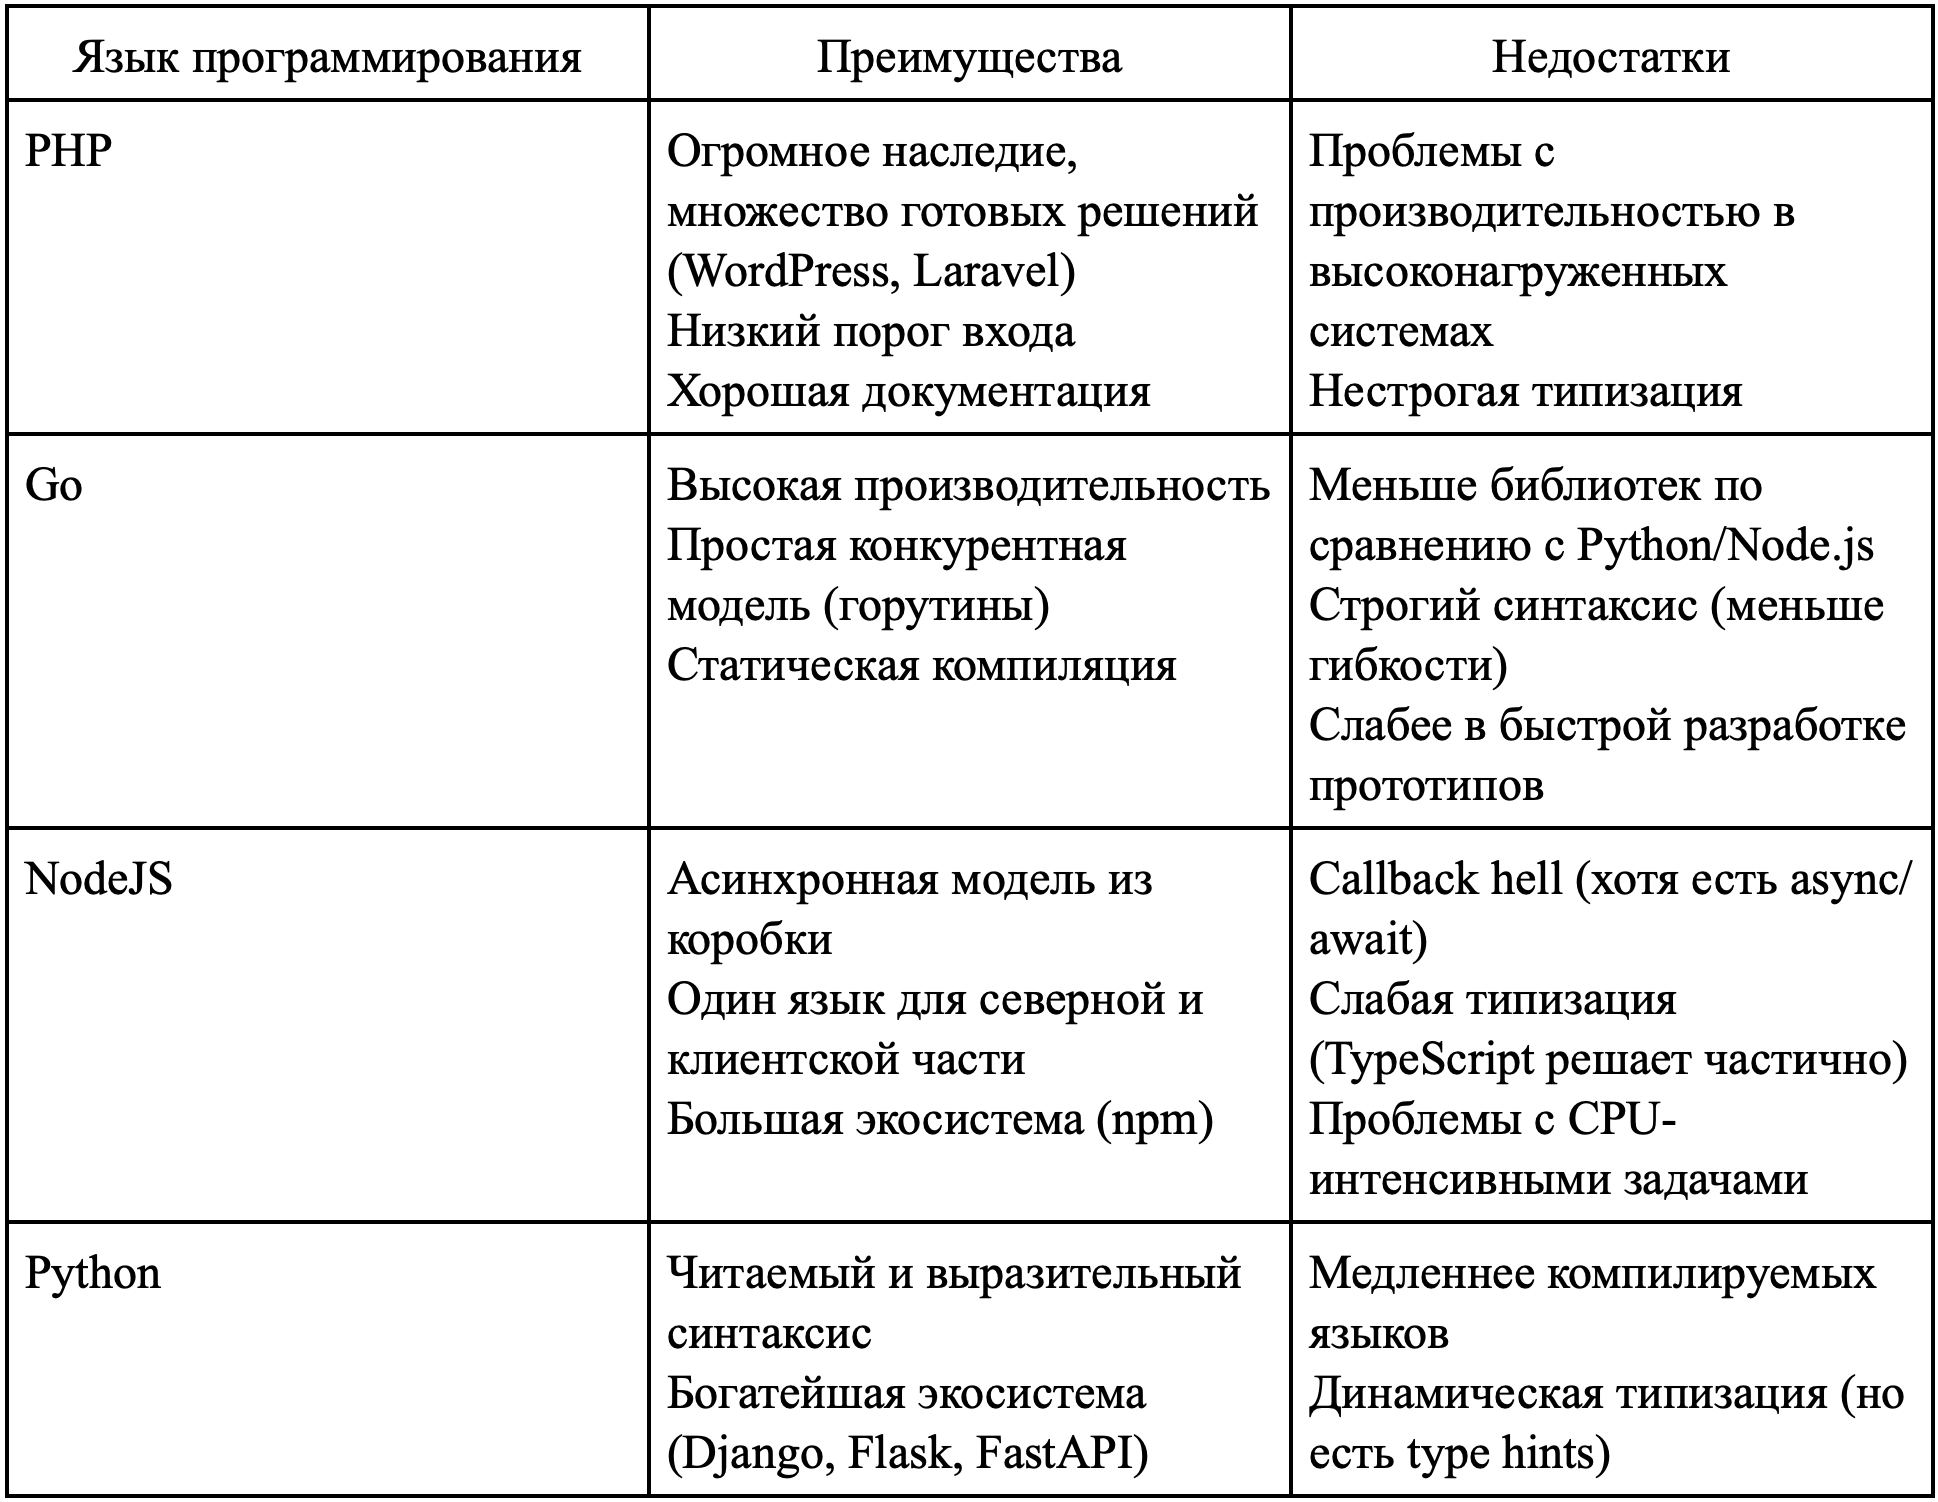
\includegraphics[width=1\linewidth]{parts/Таблица 1.jpg}
}
\hspace{-11pt}

% \noindent Таблица 1 - Сравнительная характеристика технологий на серверной части.

% \vspace{12pt}

% \noindent
% {
% \small % 12pt (~10.5pt в зависимости от класса) или \small для 11pt
% \renewcommand{\arraystretch}{0.83} % Межстрочный интервал ≈1pt (0.83 * 1.2 = ~1pt)
% \begin{tabularx}{1\textwidth} { 
%   | p{2cm}
%   | >{\raggedright\arraybackslash}X 
%   | >{\raggedright\arraybackslash}X | }
%  \hline
% \multicolumn{1}{|c|}{Язык программирования} & 
% \multicolumn{1}{c|}{Преимущества} & 
% \multicolumn{1}{c|}{Недостатки} \\
% \hline
% \multirow{3}{*}{PHP} 
% & Огромное наследие, множество готовых решений (WordPress, Laravel) &Проблемы с производительностью в высоконагруженных системах \\
% & Низкий порог входа&Нестрогая типизация \\ 
% & Хорошая документация& \\ 
% \hline
% \multirow{3}{*}{Go} &Высокая производительность &  Меньше библиотек по сравнению с Python/Node.js \\ 
% & Простая конкурентная модель (горутины) & Строгий синтаксис (меньше гибкости) \\ 
% & Статическая компиляция & Слабее в быстрой разработке прототипов \\ 
% \hline
% \multirow{3}{*}{NodeJS} &Асинхронная модель из коробки & Callback hell (хотя есть async/await) \\ 
% & Один язык для северной и клиентской части & Слабая типизация (TypeScript решает частично) \\ 
% &  Большая экосистема (npm) & Проблемы с CPU-интенсивными задачами \\ 
% \hline
% \multirow{2}{*}{Python} & Читаемый и выразительный синтаксис & Медленнее компилируемых языков \\ 
% & Богатейшая экосистема (Django, Flask, FastAPI) &Динамическая типизация (но есть type hints) \\ 
% \hline
% \end{tabularx}
% }

В качестве основного языка программирования выбран Python. Для создания функционального веб сервиса выбран фреймворк FastAPI [19].

Выбор этого фреймворка обусловлен следующими факторами и преимуществами:
\begin{enumerate}[label=\arabic*)]
    \item быстрая разработка: Python позволяет создавать прототипы приложений мааксимально быстро;
    \item современный подход: FastAPI предоставляет документацию OpenAPI, встроенную валидацию через Pydantic, поддержку async/await;
    \item гибкость: возможность интеграции с ML-моделями, аналитическими инструментами и внешними сервисами;
    \item сообщество: огромное количество готовых решений и библиотек;
    \item производительность: FastAPI сравним по скорости с Node.js и Go в типичных web-задачах.
\end{enumerate}

Python и FastAPI — это оптимальный баланс между скоростью разработки, производительностью и поддерживаемостью кода для учебного проекта.

Определившись с списком технологий, рассмотрим архитектуру серверной части приложения. На рисунке 17 представлена MVC [20] схема движения данных внутри сервера.

\vspace{12pt}
{
    \centering
    \fbox{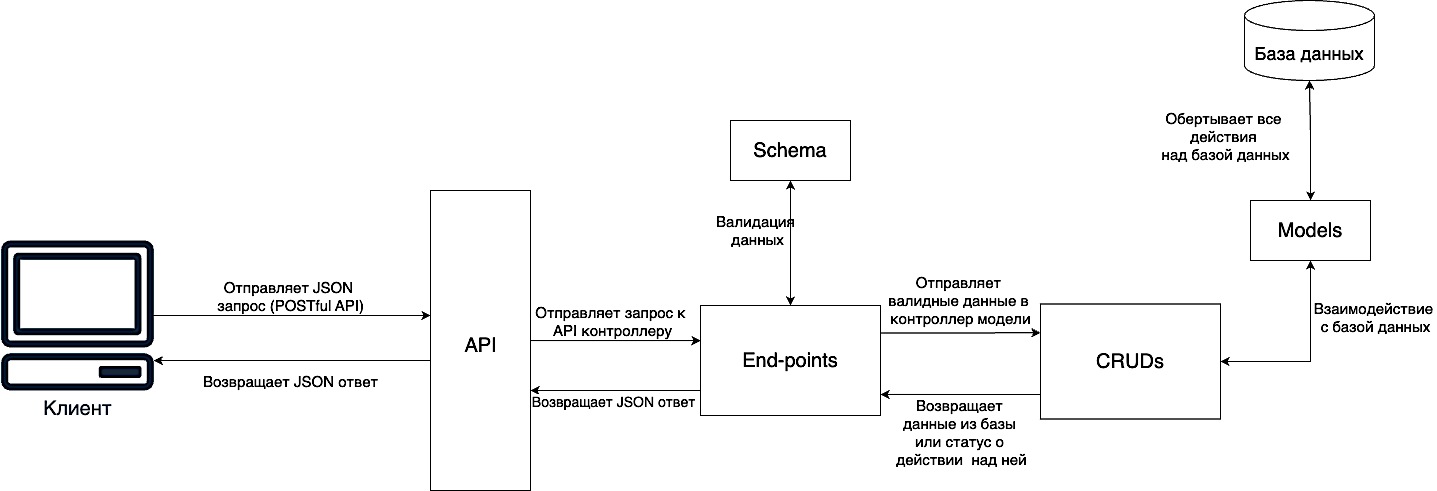
\includegraphics[width=1\linewidth]{images/Diploma-Слои backend.png}}
    \captionof{figure}{Схема взаимодействия данных от клиента до базы данных}
    \label{fig:enter-label}
}

С клиента поступает JSON запрос на получение, изменение, удаление или создание определенных данных. По указанному запросу выполняется одна точка входа в серверное приложение.
Прежде чем работать с данными - их необходимо отвалидировать, проверить, что данные удовлетворяют требованиям. За это отвечают схемы валидации - Schemas на диаграмме. В случае если данные не валидны - API возвращает 404 [21] ошибку пользователю, иначе продолжит выполнение операции. 

В зависимости от точки входа, выполняется бизнес логика взаимодействия с базой данных. Она происходит в части CRUD [22] на диаграмме. CRUD - акроним от Create Read Update Delete,  что переводится как  создание, чтение, обновление и удаление соответственно. В так называемых «крудах» происходит непосредственное взаимодействие с моделями. Модель - ORM [23] представление таблицы в базе данных, обеспечивающая упрощенный доступ к взаимодействию с данными. В отличии от схемы, модель позволяет не только отвалидировать данные, но предоставляет функционал к генерации SQL запросов к базе данных.

Полученные данные из базы, дополнительно форматируются на уровне «крудов», для необходимого формата чтения данных клиентской частью и передаются обратно в контроллер API - «ендпоинт». В контроллере происходит повторная валидация с помощью схем, чтобы удостовериться, что полученные данные из базы данных находятся в ожидаемом формате для клиентской части. После валидации серверная часть возвращает ответ к клиенту в формате JSON.

Далее, рассмотрим используемые модули для обеспечения внутреннего взаимодействия классов серверной части приложения.

Идеальным ORM поставщиком является sqlAlchemy [24] - позволяет использовать модельный архитектурный подход, в котором каждая таблица в базе данных представлена моделью с которой работает система. Это позволяет не использовать чистый SQL, а оперировать встроенным функционалом запросов, методы query для составления сложных SQL запросов. 

На слое валидации используются схемы от модуля Pydentic [25]. Этот модуль позволяет не описывать входные и выходные параметры в yaml файлах, вся валидация происходит в специальных классах - схемах, где указываются типы полей и pydentic схема сама валидирует введенные и возвращаемый параметры данных. Зачастую они схожи с sqlAlchemy моделями и поэтому их описание занимает гораздо меньше времени.

В качестве системы контроля версий был выбран github [26].

Для оптимизации временных затрат принято решение использовать только POST запросы (POSTful API) [27]. Это позволяет не разделять логику процессов на ризличные типы запросов. Любое получение, изменение и создание сущностей в базе данных происходит через POST запросы. Они имеют закрытое тело запроса в формате JSON, обеспечивая поддержку любого типа данных (будь это строки, числа, массивы или объекты).

Рассмотрим вспомогательные компоненты для взаимодействия по HTTP. На уровне API, первой точкой входа это «end-поинты». Они являются публичными методами, которые использует клиентская часть проекта.

В проекте, в папке endpoints лежат все файлы относящиеся к сущностям. Например, enter\_requests отвечает за принятие и отклонение запросов на вступление в закрыте группы пользователей. 

Однако, с увеличением количества отдельных модулей возникает необходимость в оптимизации процесса добавления этих модулей в \_\_init\_\_ файл. Этот файл позволяет использовать все внутренниие файлы папки как один модуль,  ссылаясь на папку endpoints целиком. 

Для того чтобы избежать ручной ввод путей в этот файл, а также чтобы избежать появление ошибок внутри бизнес логики, что привело бы к остановке приложения в принципе, разрботан алгоритм, интегрирующий маршруты к точкам входов каждого «ендпоинта» в один общий маршрутизатор, используемый FastAPi приложением, представленый на листинге 2.7.

\begin{lstlisting}[language=Python, caption=Алгоритм сбора маршрутов,breaklines=true]
1 """
2 Entry point for all endpoints
3 """
4 import os
import importlib
5 from fastapi import APIRouter
6 from env_constants import BASE_URL
7 app_router = APIRouter()
8 def include_routers(app_router: APIRouter):
9     endpoints_path = os.path.join(os.path.dirname(__file__), 'endpoints')
10    for filename in os.listdir(endpoints_path):
11        if filename.endswith('.py') and filename != '__init__.py':
12            module_name = filename[:-3]
13            try:
14                module = importlib.import_module(
15                    f'api.endpoints.{module_name}')
16                if hasattr(module, 'router'):
17                    app_router.include_router(
18                        module.router, prefix=f'/{BASE_URL}', tags=[module_name])
19                    print(f'{module} router is added')
20            except Exception as e:
21                print(f'Failed to include router from {filename}: {e}')
22
23 include_routers(app_router)
\end{lstlisting}

Разберемся более детально в коде листинга 2.7. 

Перед тем как вызвать функцию агрегации маршрутов API, создается общий FASTApi роутер в который последовательно добавляются все роутеры из модулей в папке edpoints. Первостепенно происходит получение абсолютного путя к папке в которой хранятся «ендпоинты» (папка endpoints) на строке 10. 

Это достигается благодаря использованию встроенной библиотеки os (строка 4) и объединения абсолютного путя с названием папки.

Далее происходит запуск алгоритма итерации по списку всех файлов внутри директории «ендпоинтов» (строка 11).

В случае если имя файла содержит в себе подстроку \_\_init\_\_ этот файл пропускается и процесс итерации продолжается далее (строка 12).

Далее с помощью бибилотеки importlib динамически загружется содержимое файла в оперативную память (строка 15). В случае если в модуле содержится переменная router, включемый в общий роутер.

Таким образом, область включения маршрутов включает в себя все существующие маршруты без необходимости вручную импортировать их в общий инит файл.

Далее,  если один из роутеров содержит в себе ошибку, сработает обработчик Exception (строка 21) и выведет в консоль трейс ошибки и причину по которой маршрут не смог собраться. 

Далее в приложении уже используется обще собранный роутер со всеми рутами к ендпоинтам.

Каждый роутер использует бизнес логику из отдельных файлов в папке cruds. Каждый из них наследуется от базового круда.

Рассмтотрим файл crud/base.py, листинг которого представлен в приложении В листинг 1. В нем описан класс BaseCRUD, в котором существуют основные методы взаимодействия с базой данных.

Как было упомянуто ранее, CRUD [28] - является акронимом от производных слов: Create, Read, Update, Delete - создание, чтение, обновление и удаление соотстветственно. В данном случае, стоит добавить еще букву L - List - чтение сразу нескольких элементов из базы данных.

Данный класс является общим и напрямую никогда не вызывается. От него наследуются [29] другие классы CRUD-ы, которые оперируют с одной или с несколькими моделями сразу. Базовый круд поддерживает одновременную работу как с одной моделю, так и с несколькими.

Рассмотрим по отдельности все основные публичные этого класса. Круды наследники могут переопределять и использовать все методы, а уже классы контроллеров могут использовать только публичные методы.

Инициализация класса. По умолчанию, при инициализации базового круда, ему необходимо передать:

\begin{enumerate}[label=\arabic*)]
    \item db - экземпляр сессии базы данных;
    \item model - основная модель с которой базовый круд будет работать;
    \item joined\_models - список моделей с полями для фильтрации.
\end{enumerate}

Публичный метод получения одной записи. Метод get\_item предназначен для получения одной записи из таблицы, указанной при инициализации класса или в парамтрах вызова. 

На вход он получает body запроса - как правило там только id записи,
field - строка, поле по которому будет проходить поиск, по умолчанию id.

Сперва метод создает экземпляр query - запроса (SELECT * FROM model) на который будут накладываться другие фильтры.

Для начала следует проверить, что переданное поле field описано в модели, а также о том, что в body запросе это значение существует.
Если нет, то возвращается 404 ошибка NotFoundError.

Далее, происходит попытка получения объекта модели с помощью применения фильтра wheres к query по полю которое получено из тела запроса и значению из тела запроса запроса.

Полученный объект возвращается.

Метод get использует метод get\_item, с разницей лишь в том, что полученный объект он обарачивает через наследуемый метод \_make\_output - для кастомного преобразования полученного элемента.

Метод получения списка данных. Метод list используется для получения одного или нескольких значений из базы данных. 
На вход поступает POST запрос с телом в формате JSON, в котором данные сформированы в специальном формате фильтров и сортировок.

Метод вызывает публичный метод get\_items и полученный результат также обарачивает в метод \_make\_output - для кастомного преобразования каждого полученного элемента, а затем в необходимый формат для клиентской части.

Метод get\_items же, сначала получает массив фильтров из тела запроса - как правило это массив из объектов, в котором column - это поле по которому будет проходить фильтрация, value - это значение с котормы необходимо сравнить, а condition - это тип сравнения значения value с значениями в базе данных.

В коде базового круда реализовано несколько типов сравнений:

\begin{enumerate}[label=\arabic*)]
    \item == полное сравнение, устанавливается по умолчанию;
    \item != отрицательное сравнение, не равно переданному значению;
    \item in значение встречается частично в базе - для массивов и объектов;
    \item \% строка встречается в другой строке;
    \item between значение находится между двух значений в массиве value.
\end{enumerate}

Этот метод к query применяет поочереди все филььтры, делает запрос к базе данных и возвращает все совпадения.

Метод обновления записи. Метод update сначала находит элемент из тела запроса в базе данных. Если такого нет, то возвращается 404 ошибка, иначе далее по каждому полю которое передано в теле запроса, достается значение, проверяется что оно не пустое и что поле не является неизменяемым. Если эти условия выполняются, то создается правильый валидный экземпляр который подлежит обновлению в базе данных.

Рассмотрев класс, позволяющий работать с базой данных и воплощать логику отдельных запросов, рассмотрим отдельный файл, позволяющий локально авторизовывать и регистрировать пользователей.

Рассмотрим файл crud/auth.py, листинг которого представлен в приложении В листинг 2.  В нем описан класс Authorisation регистрации, авторизации и прочих манипуляций с базой данных для предоставления функционала авторизованного пользователя. 

Для начала рассмотрим список ключевых используемых библиотек и модулей:

\begin{enumerate}[label=\arabic*)]
    \item sqlalchemy - ORM работа с базой данных;
    \item models - классы моделей для работы с базой данных;
    \item schemas - Схемы валидации данных на вход и выход;
    \item fastapi - Depends - класс установки зависимости для ендпонитов;
    \item BaseCRUD - базовый круд;
    \item exc - кастомные исключения, отправляемые клиенту;
    \item jose - библиотека для работы с JWT токенами;
    \item env\_constants - конфигурационные константы;
    \item bcrypt - библиотека для шифрования паролей.
\end{enumerate}

Рассмотрим существующие методы и функции.  Зависимость авторизованного доступа. Функция authorised\_user обеспечивает только авторизованный доступ к ендпоинтам внутри системы. В случае если пользователь будет пытаться получить любую информаци из защищенных ендпоинтов без токена авторизации, ему будет возвращен 401 код ошибки Unautherized. 

На вход функция получает token защифрованный токен авторизации, при расшифровке которого получается информация о дате его выдаче и о логине пользователя которому он был выдан. 
На выход функция либо возвращает экземпляр авторизованного пользователя, либо возвращает исключение-  401 ошибка код авторизации.

Токен авторизации пользователь передает в хедерах части запроса.

Первым делом, функция обращается к классу Authorisation и вызывает метод is\_token\_revoked.

Этот метод обращается к таблице revoked\_tokens и получает все токены авторизации которые уже были завершены и более не являются действительны, и пытается найти там токен предоставленный пользователем.

Если токен пользователя найден среди отозванных, то предоставленный токен уже недействителен и пользователю возвращается соответствующее сообщение с 401 ошибкой.

Иначе, если токен не был отозван, то следующим шагом, токен расшифровывается с помощью библиотеки jwt - метод decode. Он расшифровывается с учетом серкетного кода, который устанавливается при запуске приложения в env файле окружения. Для упрощения работы, был использован вместо него, пароль от базы данных к приложению.

Из полученной сигнатуры пользователя payload можно получить login пользователя, JWT [30] токен которого у нас получен.

Далее, если JWT токен невалиден, а также login не получен, то этот токен заносится в таблицу revoked\_tokens и на клиент возвращается 401 ошибка авторизации.

Иначе, по полученному login-у пользователя, идет образение к базе данных для поиска пользователя с таким логином. Если такого пользователя не существует, клиенту возвращается соответствующая ошибка с 401 кодом, иначе возвращается информация об авторизованном пользователе.

Соотстветственно, если метод выполнился успешно и без ошибок, то токен авторизации валиден, пользователю разрешно использование других методов API.

Регистрация. Метод register класса Authorisation, который отнаследован от класса BaseCRUD, получает как входной параметр экземпляр класса UserCreate - объект с полями login, password, password\_confirm.

Получив значения, для начала метод проверяет сущсвует ли уже в базе пользователь с полученным логином. Если нет, то необходимо проверить, что полученные два пароля совпадают друг с другом.

Если пароли совпадают и такого пользователя нет в базе данных, создается новый хеш пароль [31] полученного пароля, для того чтобы сохранить только хеш в базе данных. 

Метод хеширования паролей. Функция \_hash\_password принимает на вход строку - пароль в явном виде и возвращает хешированный пароль с помощью библиотеки bcrypt.

Он генерирует пароль с генерацией специальной соли - рандомной величины которая гарантирует безопасность хранения паролей пользователей.

Авторизация. Метод авторизации login принимает на вход экземпляр класса UserLogin - объект из двух полей login и password.


Для начала, необходимо проверить, что пользоваель существует и что переданный пароль совпадает с тем, что хранится в базе данных. - метод \_verify\_token.

Если этот метод возвращает экземпляр авторизованного пользователя, то необходимо вернуть этот объект пользователю, а также сформировать новый токен авторизации с которым далее пользователь сможет получать данные по другим ендпоинтам.

Этот алгоритм прост, для начала необходимо определить время когда это токен станет невалидным. С помощью этого значения, передается в метод \_create\_access\_token - полученный токен далее возвращается пользователю.

Метод проверки на существование пользователя и совпадение паролей. Метод \_verify\_token получает на вход login и password пользователя, статус авторизации которого пока не определена. Для начала получаем информацию о пользователе из базы данных. Если она есть, значит пользватель существует и можно сравнивать пароли. Иначе возвращается 401 ошибка.

Пароли сравниваются следующим образом: По полученному прямому паролю пользователя создается хеш с солью и сравнивается с тем, что хранится в базе данных. Если эти хеши совпадают - пользователю гарантирован вход, иначе 401 ошибка. 



\section{Разработка интерфейса}

Рассмотрим процесс создания уникальной айдентики приложения.

В рамках разработки веб-приложения администрирования групповых занятий особое внимание было уделено оформлению пользовательского интерфейса, цветовая палитра [32] формирует у пользователя визуальной идентичности проекта. Сформированная палитра представлена на рисунке 18.

\vspace{12pt}
{
    \centering
    \fbox{
\includegraphics[width=0.65\linewidth]{images/design/colors.jpg}}
    \captionof{figure}{Цветовая палитра}
    \label{fig:enter-label}
}

Основной цвет: Темно-зеленый (\#1C231C). Используется для заголовков, ключевых кнопок и важных элементов интерфейса. Этот глубокий оттенок зелёного ассоциируется с стабильностью, профессионализмом и экологичностью, что делает его идеальным для образовательных платформ. Он обеспечивает хороший контраст на светлом фоне и помогает пользователям быстро находить ключевые зоны взаимодействия.

Фоновый цвет: Светло-серый (\#F4F7F7). Применяется в качестве основного фона интерфейса. Его нейтральность и мягкость снижают визуальную нагрузку, создавая комфортную среду для работы с контентом. Этот цвет также улучшает читаемость текста и других элементов, размещённых на нём.

Границы и разделители: Светло-серый (\#D3D3D3). Используется для линий, рамок и визуального разделения блоков (например, между строками в расписании или секциями меню). Его лёгкость помогает структурировать информацию, не перегружая интерфейс.

Мобильные разделители: Светло-серый (\#E0E0E0). Оптимизирован для мобильных устройств — применяется для тонких линий в компактных представлениях (например, в списках учеников или настройках). Чуть светлее, чем \#D3D3D3, чтобы лучше сочетаться с небольшими экранами.

Фоновое размытие: Чёрный с прозрачностью (\#000000, 50\% opacity + blur 30). Необходимо для модальных окон, всплывающих подсказок и затемнения фона. Размытие помогает сфокусировать внимание на активном элементе (например, форме добавления урока), а прозрачность сохраняет связь с контекстом.

Далее, рассмотрим процесс создания макетов страниц.

На рисунке 19 представлен макет страницы для входа в систему. 

\vspace{12pt}
{
    \centering
    \fbox{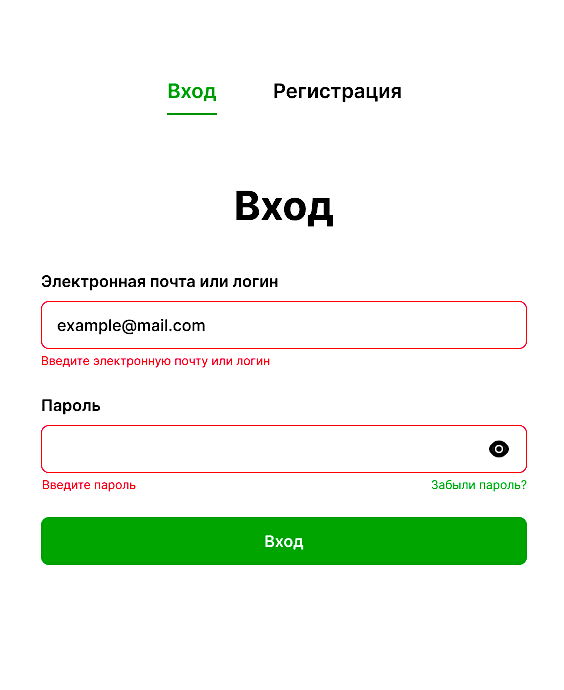
\includegraphics[width=0.65\linewidth]{images/design/Вход.png}}
    \captionof{figure}{Прототип страницы Вход}
    \label{fig:enter-label}
}

Это форма с двумя полями, у каждого поля для ввода есть подсказки, а также указаны ошибки если введенные значения некорректны.

На рисунке 20 представлен макет страницы для регистарции в системе. 

\vspace{12pt}
{
    \centering
    \fbox{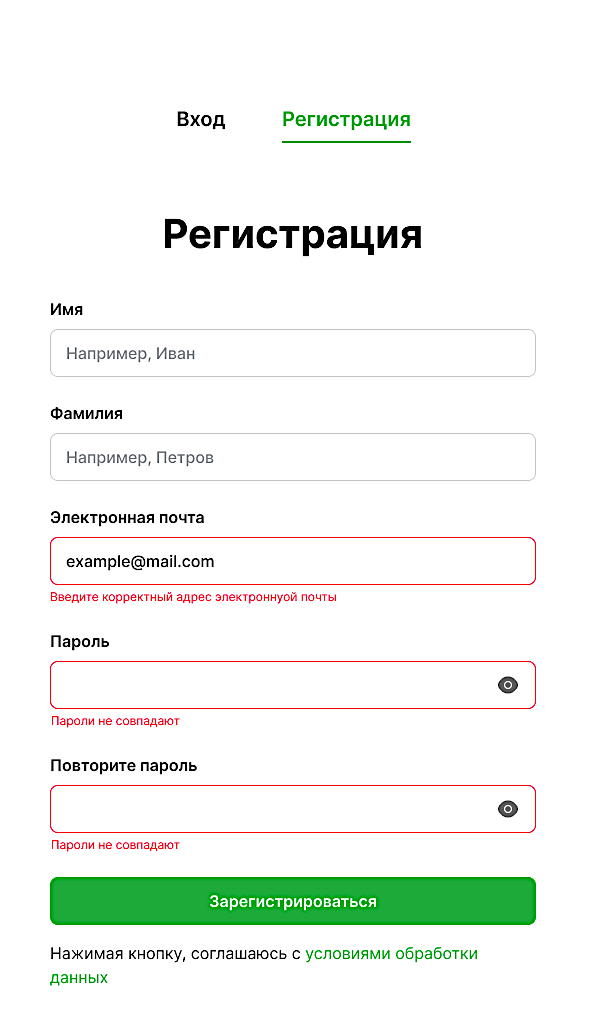
\includegraphics[width=0.5\linewidth]{images/design/Регистрация.png}}
    \captionof{figure}{Прототип страницы Регистрация}
    \label{fig:enter-label}
}

В форме представлены основные поля необходимые лдя регистрации нового пользователя. При вводненесовпадающих пароей, высвечивается соответствующее сообщение о валидации. Также, под кнопкной о регистрации можно найти ссылку на условия обработки персональных данных.


На рисунке Б.2 представлен макет страницы расписания пользователя, одного из 3 основных разделов сервиса. На вкладке расписание находится интерактивный компонент с календарем, позволяющий переключаться между месяцами, а также кнопкой создания занятия на выбранную дату. Справа от него находится более подробный компонент календаря с переключением между днем (рисунок Б.2), неделей (рисунок Б.3) и месяцем (рисунок 21). 

\vspace{12pt}
{
    \centering
    \fbox{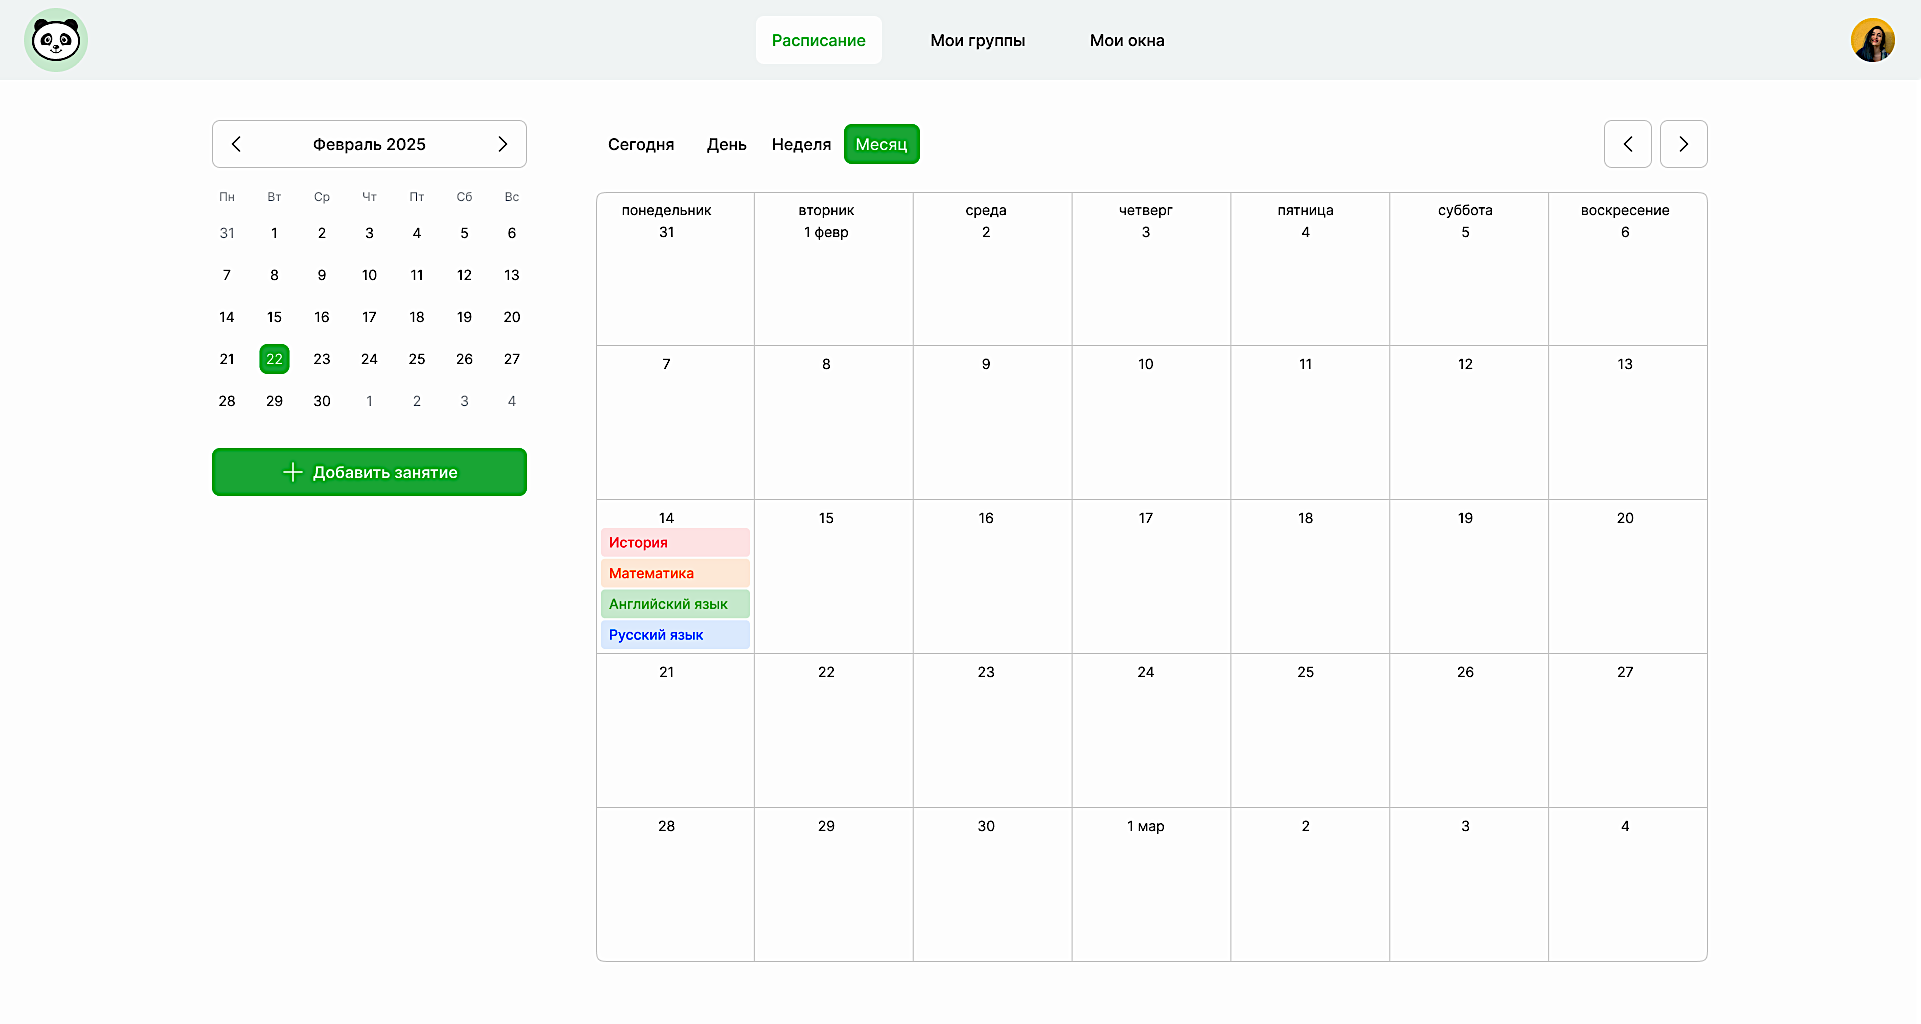
\includegraphics[width=1\linewidth]{images/design/Расписание_Месяц.png}}
    \captionof{figure}{Прототип страницы «Расписание». Календарь, месяц}
    \label{fig:enter-label}
}

На каждом рисунке представлены предстоящие занятия среди всех групп, а также свои открыте слоты. Здесь представлен календарь, позволяющий выбирать дату, отображаемую в общем календаре. 

На рисунке 22 представлен макет страницы групп с точки зрения Преподавателя.

\vspace{12pt}
{
    \centering
    \fbox{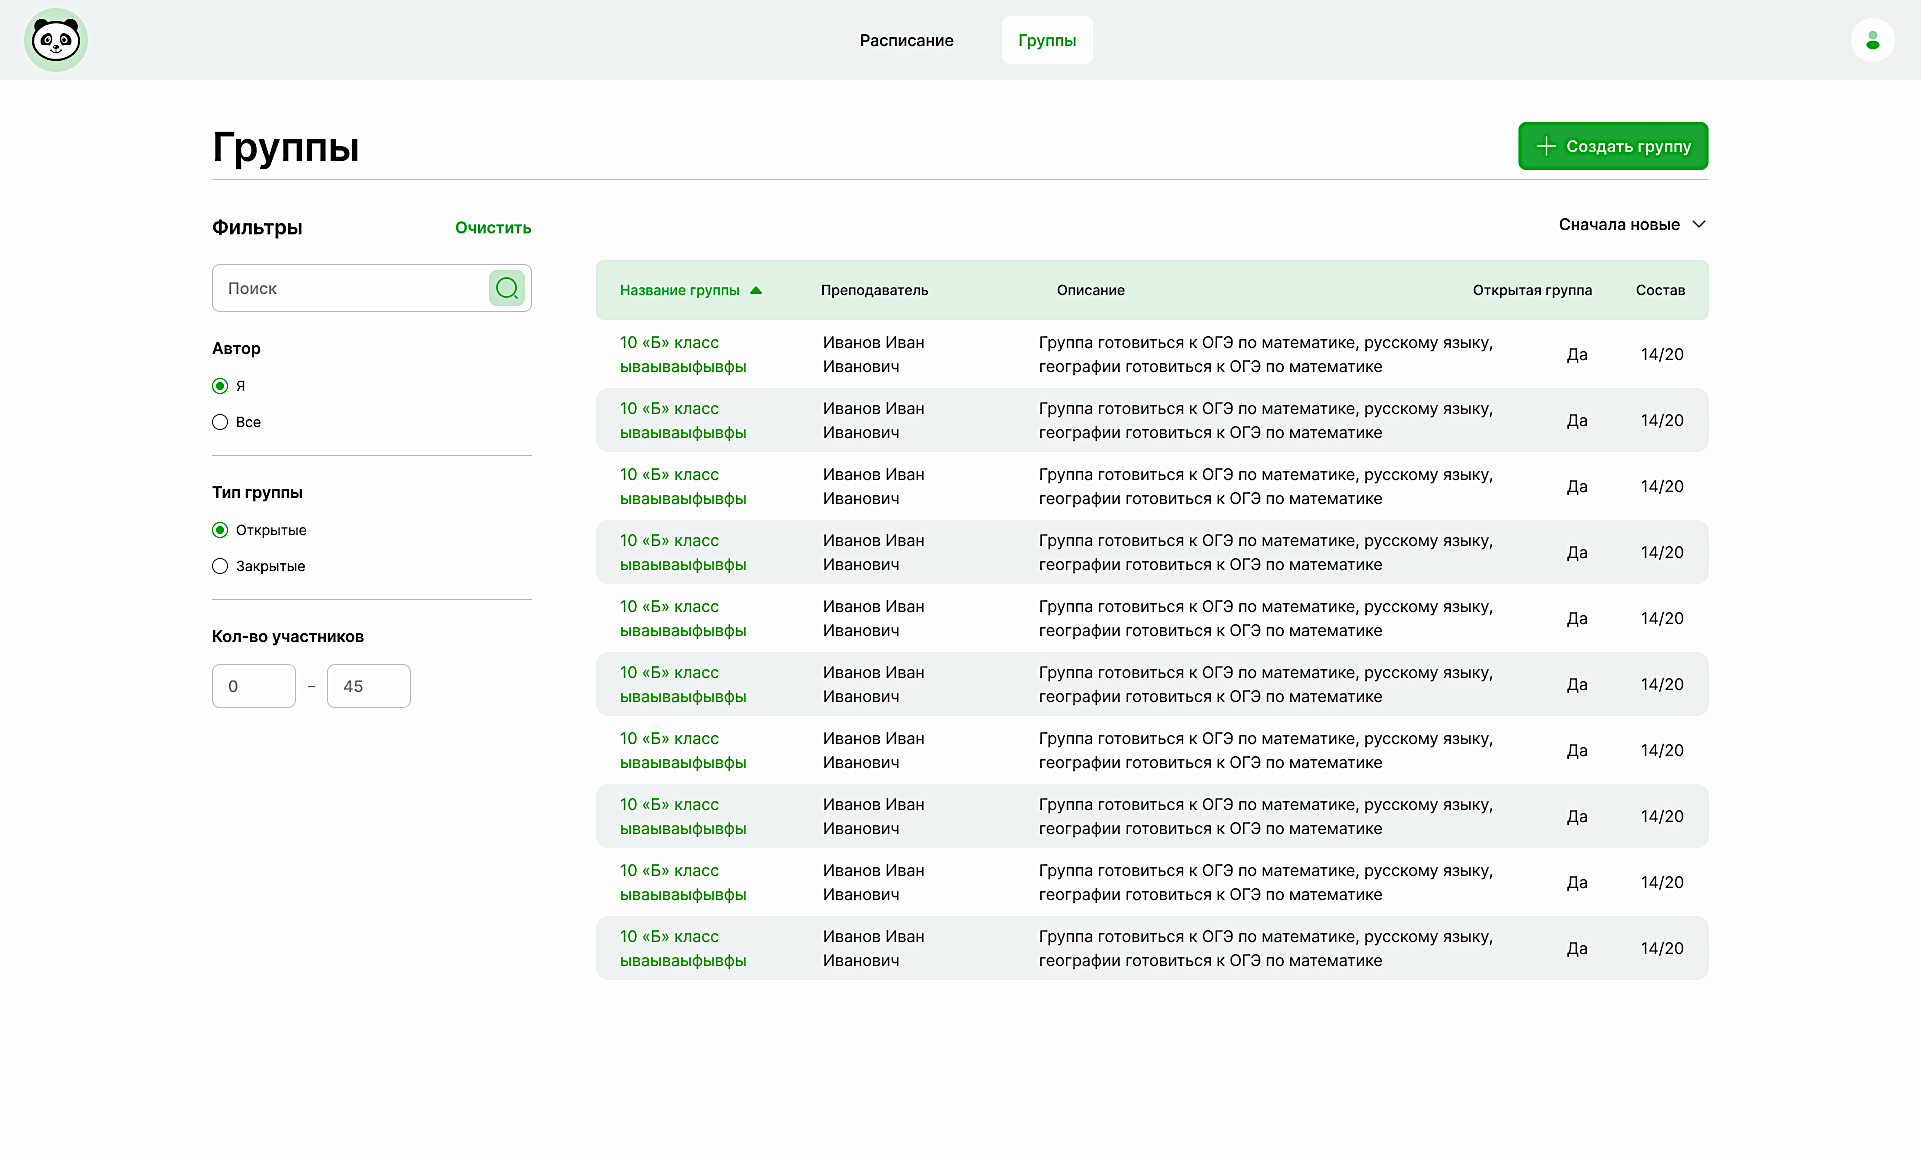
\includegraphics[width=1\linewidth]{images/design/Мои группы.png}}
    \captionof{figure}{Прототип страницы таблицы групп от лица преподавателя}
    \label{fig:enter-label}
}

Здесь, в левой части страницы располагается форма для фильтрации групп по характеристикам:
\begin{enumerate}
    \item По автору группы: им является текущий пользователь или другие пользователи.
    \item По области видимости: будут отображаться группы с свободным входом или с одобрением администратора.
    \item По количеству участников в группе.
\end{enumerate}

Справа от формы располагается сама таблица с полями: Название, Преподаватель, Описание группы, является ли она открытой или закрытой, а также её состав - общее количество участников к максимальному.

Над таблицей можно наблюдать кнопку создания новой группы. Она видна только пользователю с ролью преподавателя.

При клике на группу в таблице, происходит переход в карточку группы, представленную на рисунке 23. 

\vspace{12pt}
{
    \centering
    \fbox{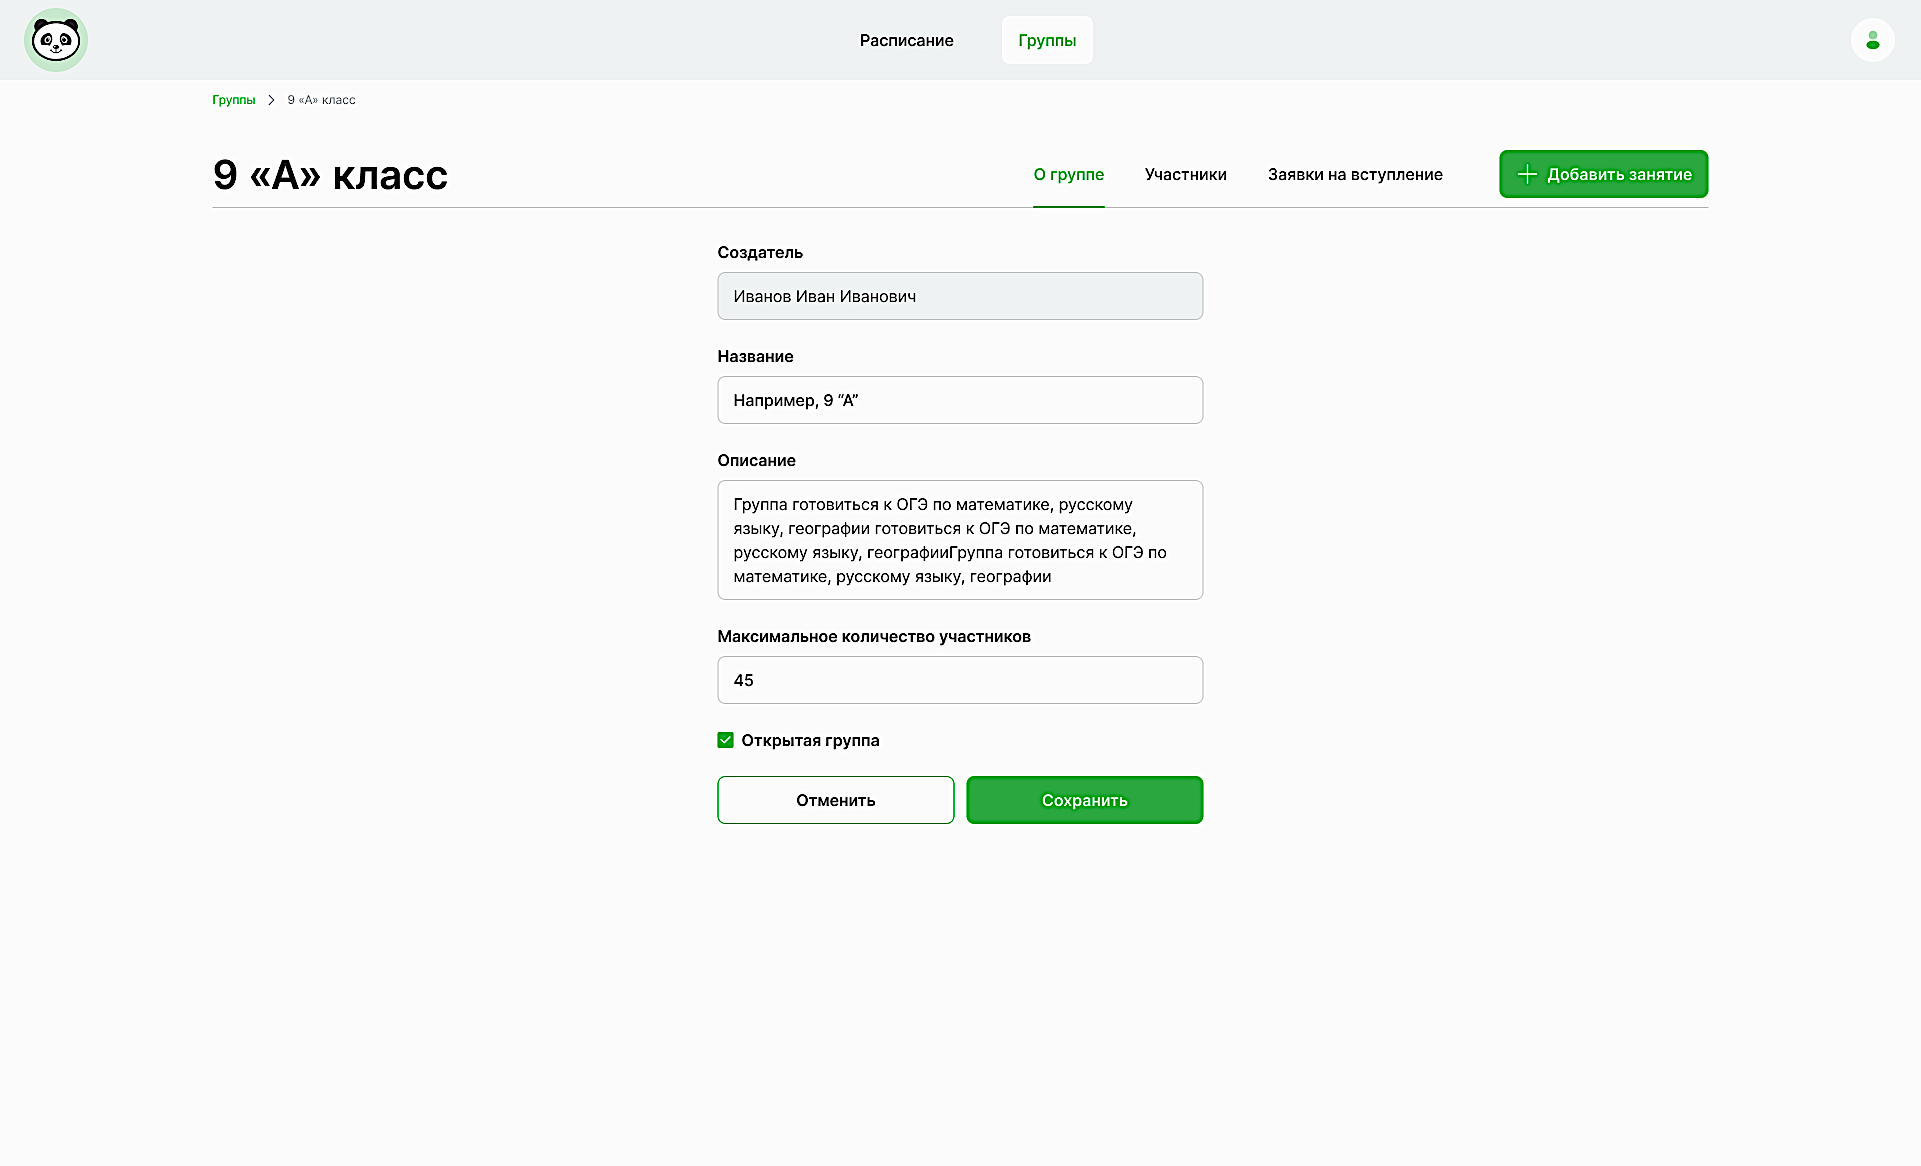
\includegraphics[width=1\linewidth]{images/design/Редактирование группы.png}}
    \captionof{figure}{Прототип страницы редактирования группы от лица преподавателя}
    \label{fig:enter-label}
}

Если пользователь является её автором, он может отредактировать информаицю о группе, а также ему предоставляется функционал управления участниками, занятиями, а также запросами на вступление, если группа является закрытой.


На рисунке 24 представлен прототип страницы просмотра участников группы.

\vspace{12pt}
{
    \centering
    \fbox{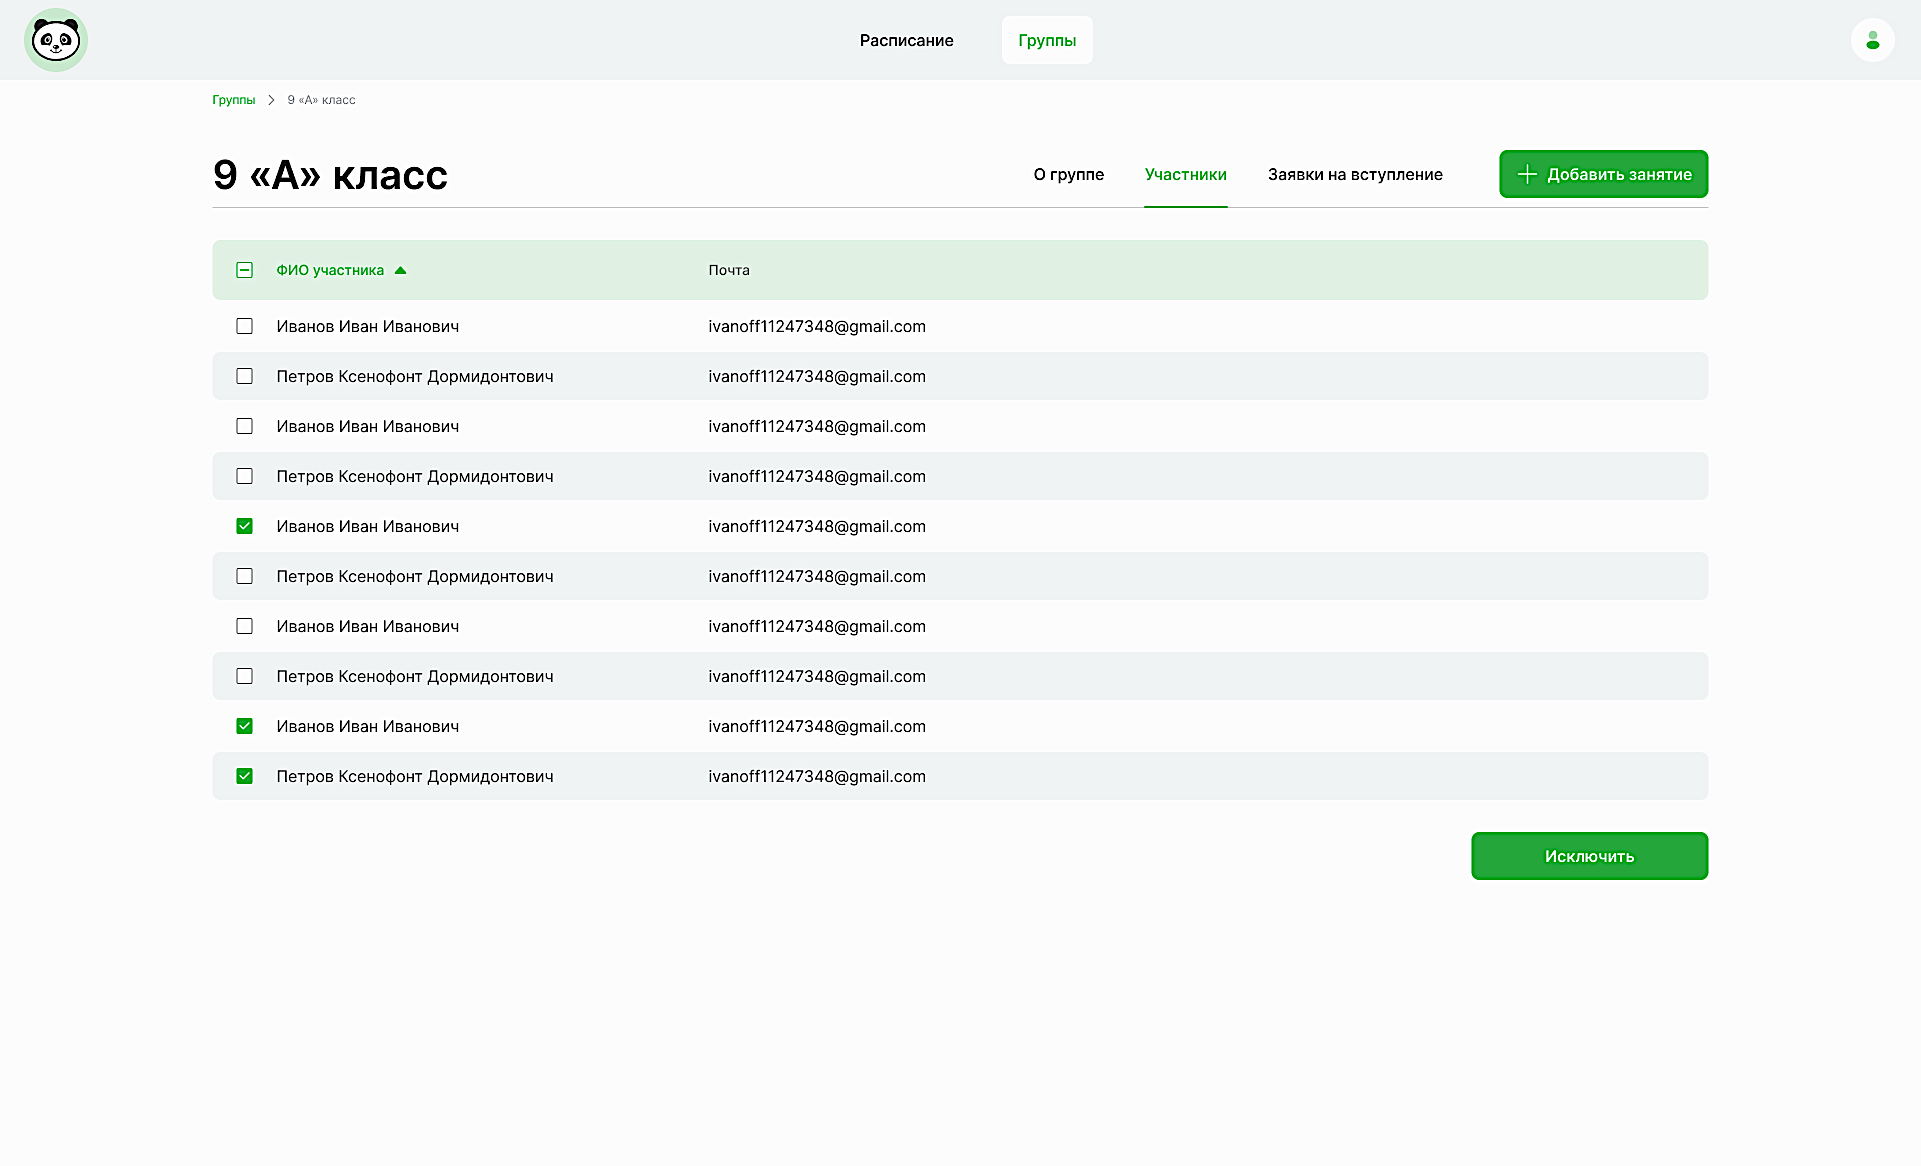
\includegraphics[width=0.8\linewidth]{images/design/Участники группы.png}}
    \captionof{figure}{Прототип страницы участников группы от лица преподавателя}
    \label{fig:enter-label}
}

Здесь, пользователь может прямо в таблице выбрать участников, чтобы удалить их из группы, по нажатию кнопки.


Далее на рисунке 25 представлен прототип страницы просмотра заявок на вступление в группу. 

\vspace{12pt}
{
    \centering
    \fbox{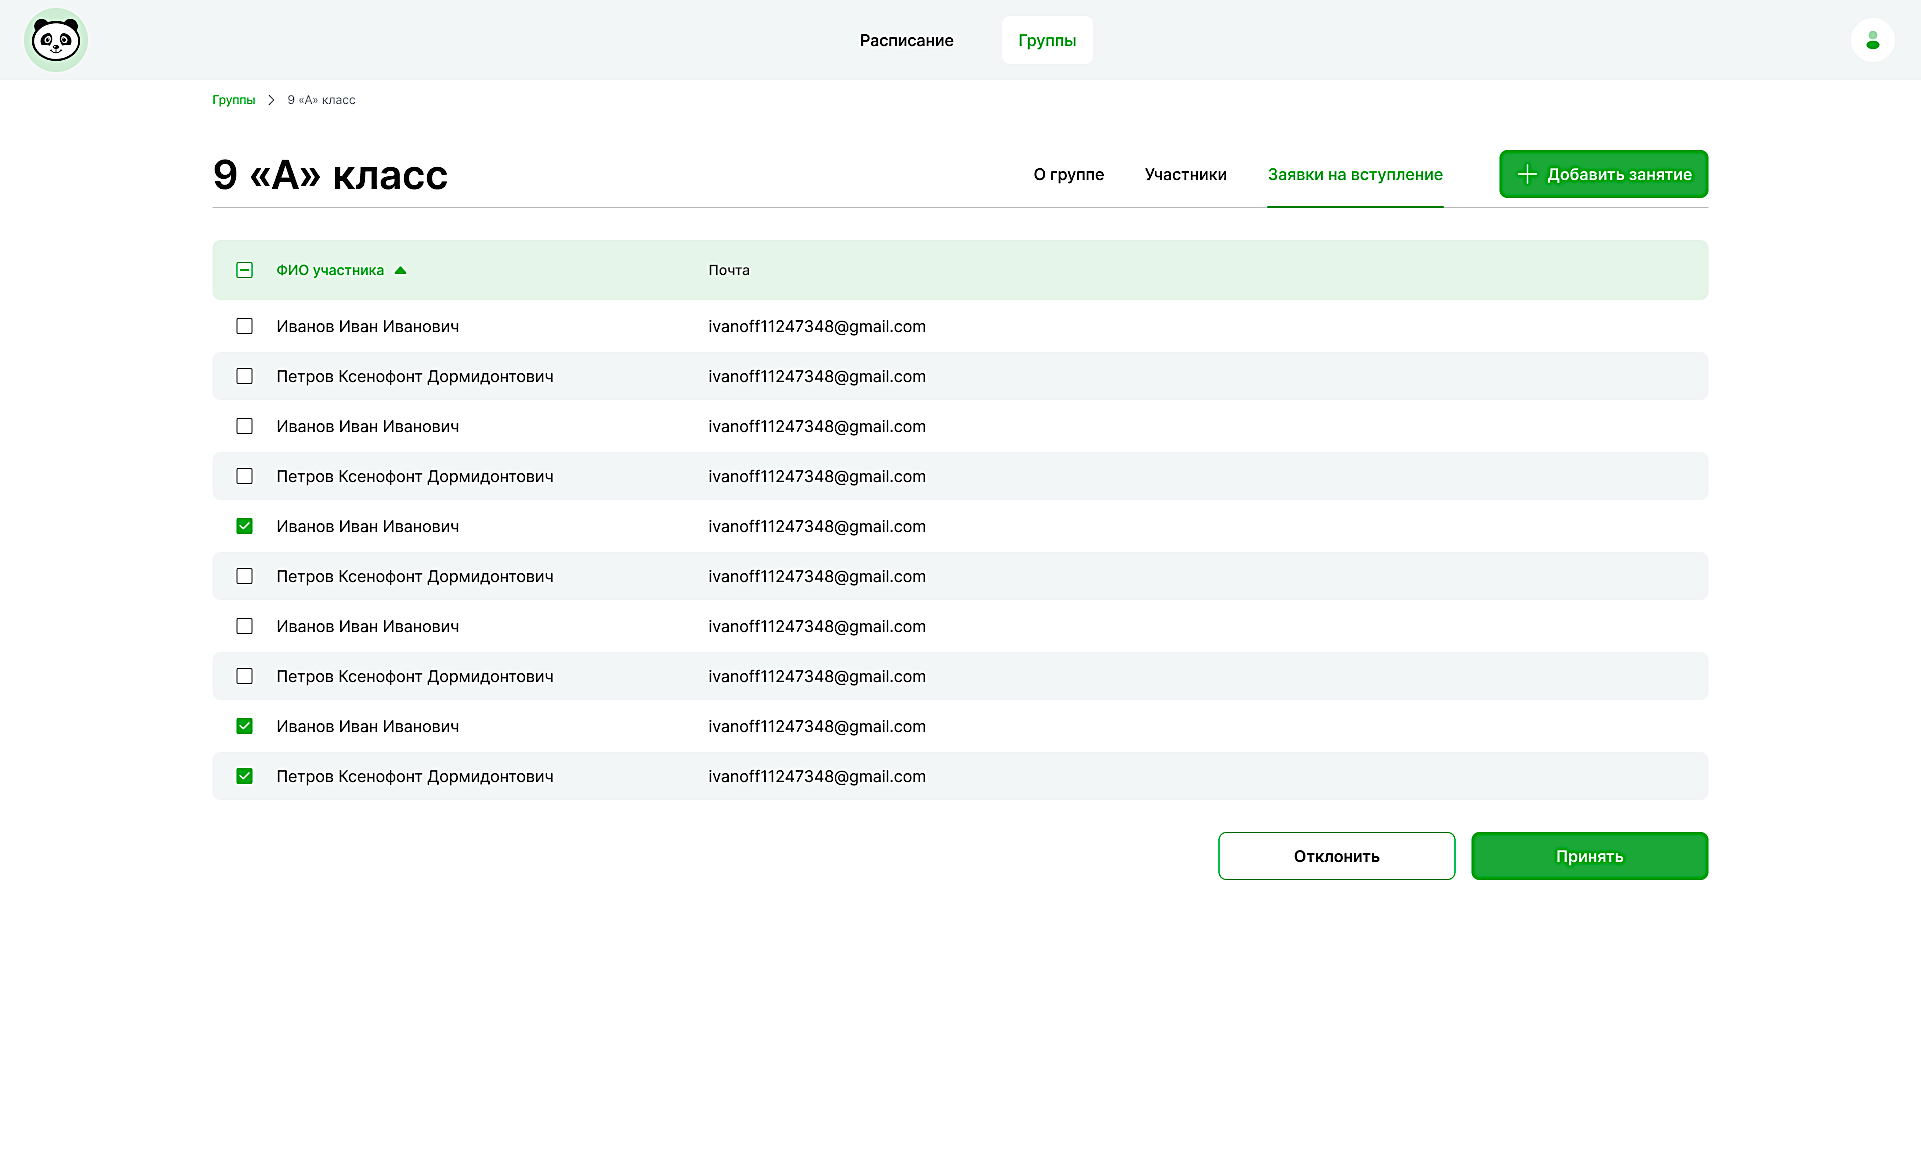
\includegraphics[width=0.9\linewidth]{images/design/Заявки на вступление.png}}
    \captionof{figure}{Прототип страницы заявок на вступление в группу от лица преподавателя}
    \label{fig:enter-label}
}

Здесь, администратор группы может выбрать одного или нескольких пользователей и принять их в группу, или отклонить им доступ в группу. Об этом, пользователи увидят в своем интерфейсе.


Далее на рисунке 26 представлена форма создания занятия внутри группы.

\vspace{12pt}
{
    \centering
    \fbox{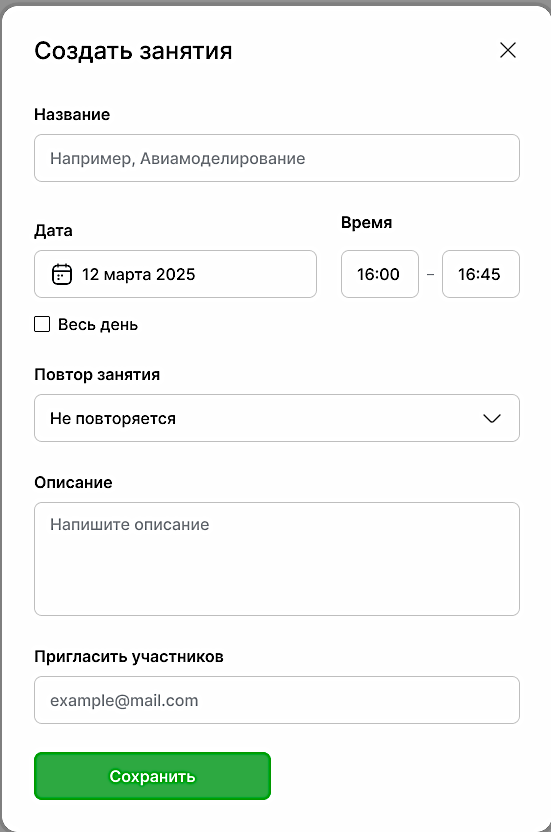
\includegraphics[width=0.8\linewidth]{images/design/Создать занятие.png}}
    \captionof{figure}{Прототип страницы создания занятия в группе от лица преподавателя}
    \label{fig:enter-label}
}

Здесь преподаватель может задать название будущему занятию, дату - когда это занятие будет проходить, а также время. Также, можно задать периодичность повторения занятия, тогда в календаре это занятие будет повторяться с заданной периодичностью. Также в описание можно расписать подробнее чем ученики будут заниматься, приложить материалы к занятию.


Далее рассмотрим страницы управления группами с стороны обучающегося. На рисунке 27 представлена схожая таблица с группами.

\vspace{12pt}
{
    \centering
    \fbox{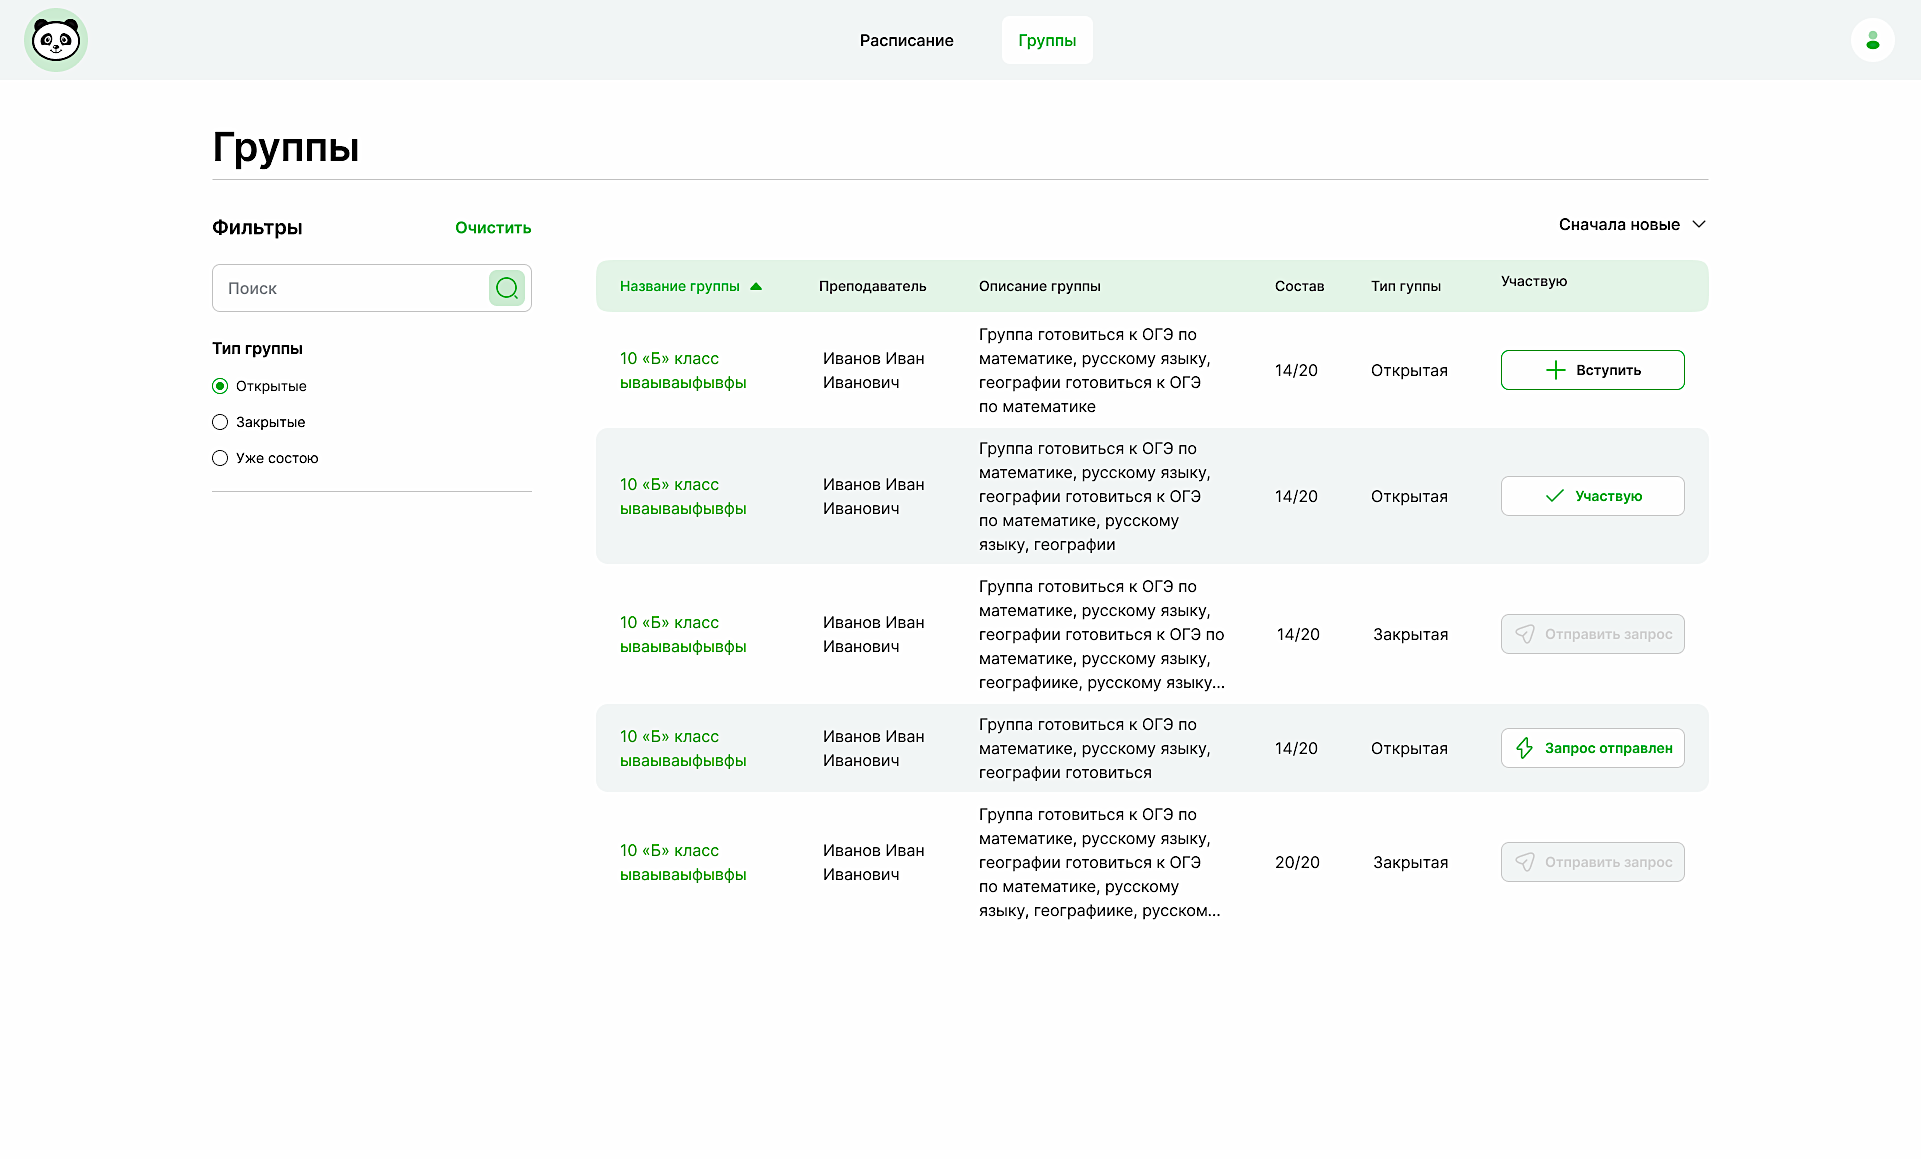
\includegraphics[width=1\linewidth]{images/design/Мои группы Учеинк.png}}
    \captionof{figure}{Прототип страницы просмотра групп от лица обучающегося}
    \label{fig:enter-label}
}

Здесь обучающийся может так же в фильтр-форме отфильтровать группы по тому являются ли они открытыми или закрытыми, или же посмотреть только те группы, в которых он состоит. 

В самом правом столбце таблицы представлена информативная кнопка, информаирующая пользователя о том, является ли он участником группы и если нет, то может ли он вступить в неё сразу или лишь отправить запрос на вступление в закрытую группу.

Также, можно наблюдать отсуствие кнопки добавления новой группы. Этот функционал предусмотрен только для пользователей с ролью преподавателя. Далее на рисунке 28 представлен прототип просмтора карточки группы, в которой ученик состоит.

\vspace{12pt}
{
    \centering
    \fbox{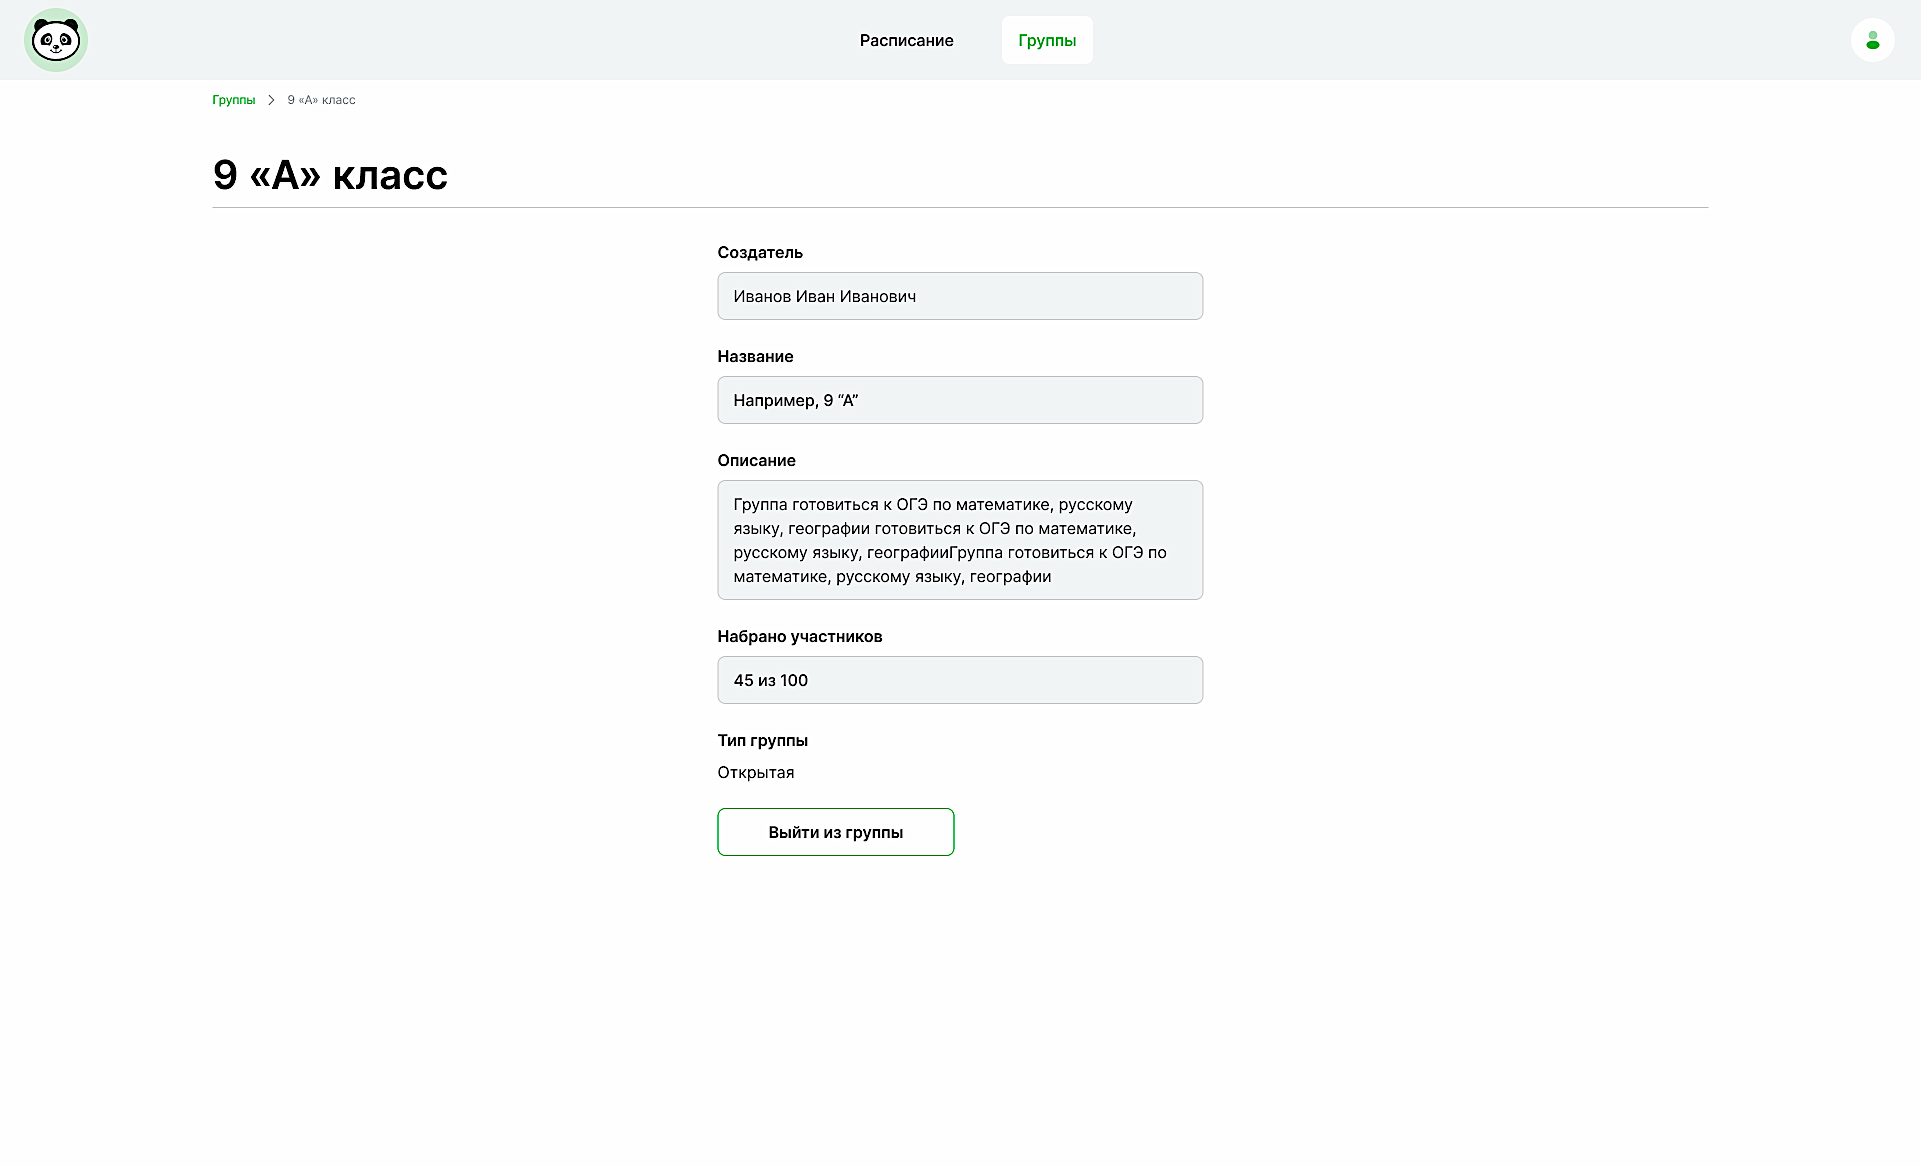
\includegraphics[width=1\linewidth]{images/design/Просмотр группы Ученик.png}}
    \captionof{figure}{Прототип страницы просмотра одной группы от лица обучающегося}
    \label{fig:enter-label}
}

Здесь пользователь имеет возможность посмотреть более подробную информацию о группе и кнопку покидания группы.


\section {Проектирование и разработка клиентской части приложения}

Прежде чем углубляться в детализированное рассмотрение ключевых аспектов к процессу проектирования и реализации пользовательского интерфейса и функциональных компонентов клиентской части веб-приложения, представляется крайне важным и методически обоснованным провести всесторонний анализ  существующих на текущий момент времени технологических решений, инструментальных платформ и фреймворков, доступных разработчикам.

В современных условиях разработки простого использования нативного JavaScript [33] уже явно недостаточно для обеспечения требуемого уровня производительности, масштабируемости и удобства разработки. В связи с этим необходимо применение фреймворков, которые значительно упрощают процесс создания клиентской части приложений.

Сравнительная характеристика JavaScript «фреймворков» [34] представлена в таблице 2.

\noindent Таблица 2 - Сравнительный анализ JavaScript фреймворков
 
\vspace{9pt}
{
    \centering
    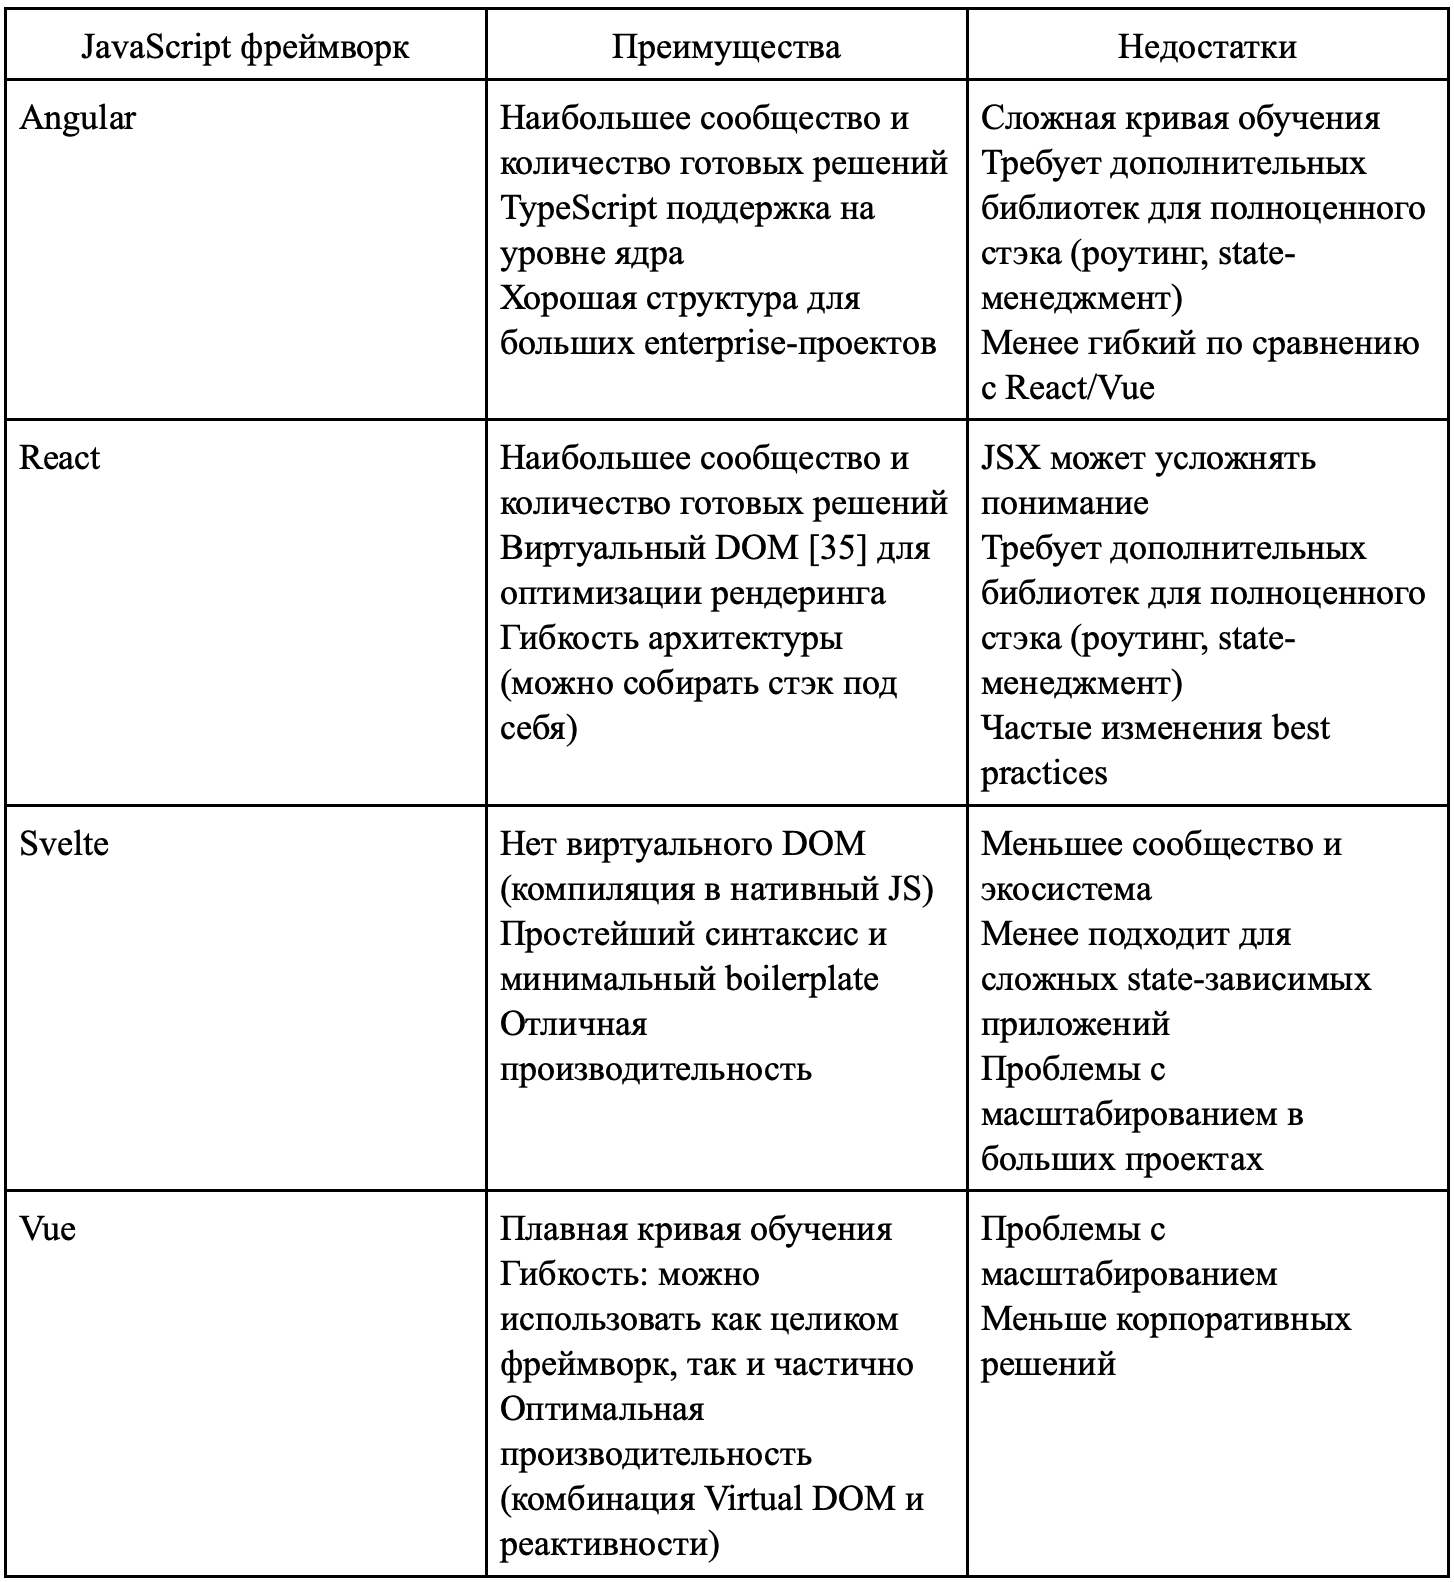
\includegraphics[width=1\linewidth]{parts/Таблица 2.jpg}
}
\hspace{-11pt}

% \noindent Таблица 2 - Сравнительный анализ JavaScript фреймворков

% \vspace{12pt}

% \noindent
% {
% \small % 12pt (~10.5pt в зависимости от класса) или \small для 11pt
% \renewcommand{\arraystretch}{0.83} % Межстрочный интервал ≈1pt (0.83 * 1.2 = ~1pt)
% \setlength{\tabcolsep}{4pt}
% \begin{tabularx}{1\textwidth} { 
%   | p{2cm}
%   | >{\raggedright\arraybackslash}X 
%   | >{\raggedright\arraybackslash}X | }
%  \hline
%  \multicolumn{1}{|c|}{ JavaScript фреймворк} & 
% \multicolumn{1}{c|}{Преимущества} & 
% \multicolumn{1}{c|}{Недостатки} \\
% \hline
% \multirow{3}{*}{Angular} & Наибольшее сообщество и количество готовых решений &  Сложная кривая обучения \\ 
% & TypeScript поддержка на уровне ядра & Требует дополнительных библиотек для полноценного стэка (роутинг, state-менеджмент) \\ 
% & Хорошая структура для больших enterprise-проектов & Менее гибкий по сравнению с React/Vue \\ 
% \hline
% \multirow{3}{*}{React} 
% & Наибольшее сообщество и количество готовых решений &JSX может усложнять понимание \\

% & Виртуальный DOM [35] для оптимизации рендеринга&Требует дополнительных библиотек для полноценного стэка (роутинг, state-менеджмент) \\ 
% & Гибкость архитектуры (можно собирать стэк под себя)&Частые изменения best practices \\ 
% \hline
% \multirow{3}{*}{Svelte} & Нет виртуального DOM (компиляция в нативный JS) &  Меньшее сообщество и экосистема \\ 
% & Простейший синтаксис и минимальный boilerplate & Менее подходит для сложных state-зависимых приложений \\ 
% & Отличная производительность & Проблемы с масштабированием \\ 
% \hline
%  \multirow{2}{1em}{Vue} & Плавная кривая обучения &  Меньше корпоративных решений \\ 
% & Гибкость: можно использовать как целиком фреймворк, так и частично & \\ 
% & Оптимальная производительность (комбинация Virtual DOM и реактивности) &  \\ 
% % & Отличная документация & \\
% \hline

% \end{tabularx}
% }

Проанализировав все доступные варианты среди сред разработки, было принято решение остановиться на Vue.js из-за следующих преимуществ:

\begin{enumerate}
    \item Простота интеграции: есть возможность постепенного внедрения.
    
    \item Композиционный API предоставляет лучшую организацию кода по сравнению с Options API, а также проще выносить логику функции.
    
    \item Оптимальная производительность: новая реактивная система на Proxy.
    
    \item Экосистема представлена Vue Router для навигации, Pinia/Vuex для state-менеджмента и Vue-CLI-Service для мгновенного hot-reload.
    
\end{enumerate}

Архитектура клиентской части приложение сформирована с помощью наслоения одних компонентов над другими. С этой схемой можно ознакомиться на рисунке 29.

\vspace{12pt}
{
    \centering
    \fbox{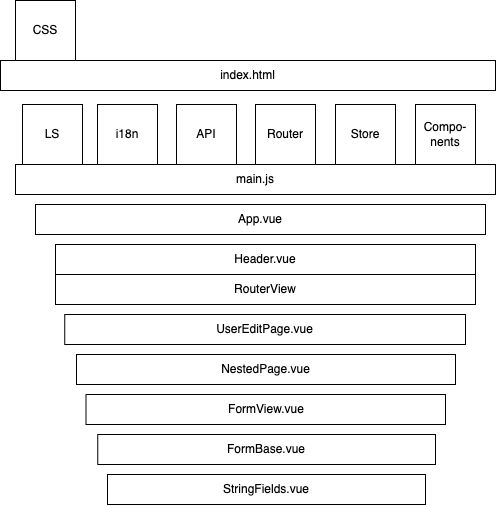
\includegraphics[width=0.7\linewidth]{images/FrontEndLayers.png}}
    \captionof{figure}{Построение компонентов на основе страницы личного кабинета }
    \label{fig:enter-label}
}

Здесь точкой входа является файл index.html - к которому монтируется Vue js приложение, а также все CSS стили.

Монтирование самого приложения происходит в файле main.js. В нем регистрируютяс все используемые глобальные модули для работоспособности приложения:

\begin{enumerate}[label=\arabic*)]
    \item LS (LocalStorage). Локальное хранилище данных в браузере. Обеспечивает хранение данных до тех пор, пока пользователь не очистит кеши страницы или не зайдет под инкогнито;
    \item i18n. Модуль позволяет реактивно изменять локаль приолжения, переключаясь моментально между языками в интерфейсе;
    \item API. По своей сути является объектом, который разделяет API для использования внутри клиентской части на смысловые части. 

    \item Router. Зарегистрированный маршрутеризатор, позволяющий монтировать определенные View компоненты к URI путям.

    \item Store. Хранилище данных между различными страницами и компонентами. Позволяет хранить глобальные состояния и описания получаемых полей с сервера. Является слоем данных;

    \item Components. Используемые компоненты, позволяющие не импортировать каждый файл при использовании компонента, а предоставив глобальный доступ к ним.
\end{enumerate}

Все вышеперечисленные модули глобальны и доступны из всех Vue компонентов из-за интеграции их на уровне файла main.js.

UserEditPage - View компонент, который определяет наполение и функционал этой страницы. В данном примере на странице редактирования представлена форма FormView.

FormView - общий компонент просмотра, редактирования и создания сущностей. Предоставляет функционал сохранения, отмены и навигации между состояниями формы. C помощью API запрашивает данные о пользователе и отображает их. При изменении данных и нажатии на кнопку сохранить отправляет запрос на обновление данных о пользователе. 

FormBase - основа для FormView. Используя Store, этот компонент определяет правила для отображения полей внутри формы, заполняет их значениями, а также валидирует их , собирая ошибки ввода.

Далее, рассмотрим функциональность приложения с точки зрения навигации по страницам приложения.

Навигационная система [36] представляет собой комплексное функциональное решение, реализующее логику переходов между разделами веб-приложения. Данный механизм играет ключевую роль в организации пользовательского взаимодействия, обеспечивая не просто возможность перемещения между страницами, но и поддерживая целостное восприятие интерфейса.

В примере выше рассматривается страница редактирования данных о пользователе, поэтому имеем RouterView - vue компонент, предоставляющий функционал рендера компонента, основанного на текущей локации пользователя внутри приложения. Все существующие страницы внутри проекта описаны на рисунке 30.

\vspace{12pt}
{
    \centering
    \fbox{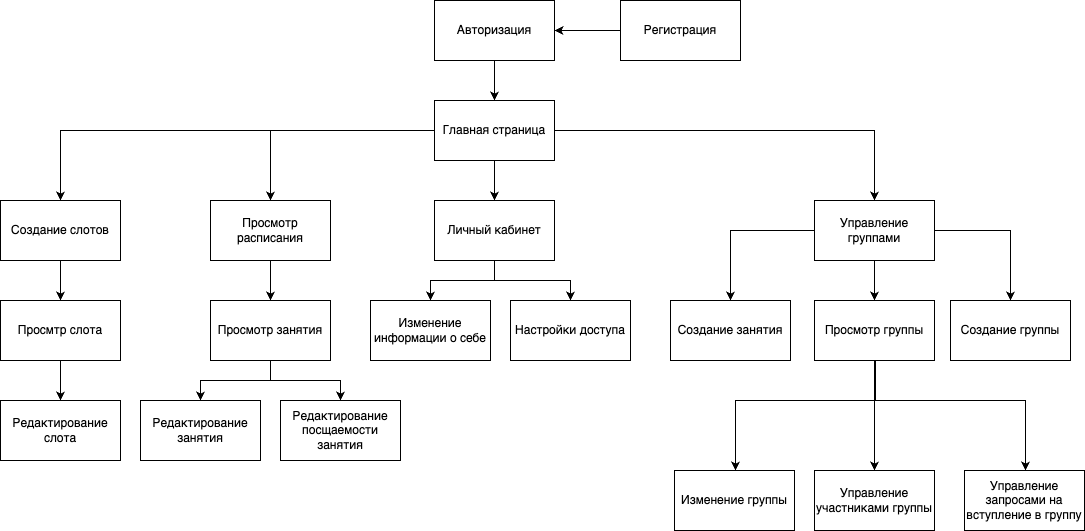
\includegraphics[width=0.9\linewidth]{images/FrotendMap.png}}
    \captionof{figure}{Карта существующих страниц в приложении}
    \label{fig:enter-label}
}

Навигация по сайту происходит по разделам:
\begin{enumerate}
    \item Группы.
    \item Слоты.
    \item Пользователь.
    \item Расписание.
    \item Авторизация.
\end{enumerate}

У разделов есть более подробные маршруты:

\begin{enumerate}[label=\arabic*)]
    \item /show - просмотр, карточка;
    \item /edit - редактирование;
    \item /new - создание;
    \item /list - просмотр списка;
\end{enumerate}

Для реализации этого функционала была использована встроенная библиотека Vue-Router. Для начала, были описаны все существующие маршруты в одной переменной sections. Представлена на листинге 2.8.

\begin{lstlisting}[language=JavaScript, caption=Все секции маршрутов в приложнии,breaklines=true]
1 const sections = [
2    { name: 'auth', actions: ['login', 'register'], useId: false },
3    { name: 'home', actions: null, useId: false },
4    { name: 'user', actions: ['show', 'edit'], useId: true },
5    { name: 'groups', actions: ['list', 'show', 'edit', 'new'], useId: true },
6    { name: 'events', actions: ['show', 'edit', 'new'], useId: true },
7    { name: 'slots', actions: ['show', 'edit', 'new'], useId: true },
8 ]
\end{lstlisting}

Здесь флаг useId определяет логику: использовать id записи в качестве последней части  маршрута или последней частью маршрута являются подразделы.

Далее, основываясь на переменной sections, генерируются все маршруты для роутера внутри приложения с помощью функции generateRoutes, представленной на листинге В.3.

Здесь идет итерация по каждой секции переменной sections и выполняются следущие проверки. 

Сначала вычесляется имя компонента - файла Vue который будет связан с каждым маршрутом. В приложении все страницы хранятся в папке /pages.
Выбирается поле name у каждой секции, первая буква делается заглавной и в конце добавляется слово Page.
Таким образом секция с названием events стала EventsPage.

Далее этот компонент по умолчанию импортируется в переменную \\defaultComponent.

Далее, если у секции есть не пустой массив actions, то по каждому действию в массиве импортируется новый компонент с следующей логикой. Например, если у секции events есть действие list, то импортируется компонент EventsListPage из папки pages/events. Иначе, если действия не описаны или массив пуст, то используется компонент по умолчанию EventsPage.

Далее, расмотрим реализованный функционал взаимодействия клиентской части приложения с серверной путем создания интерфейса отправки запросов.

API (Application Programming Interface) – это программный интерфейс, который позволяет клиентской части веб-приложения взаимодействовать с сервером по определенным правилам [37].

API построено по принципу единой точки входа с последующим роутингом на бэкенде. Основные компоненты:

\begin{enumerate}[label=\arabic*)]
    \item api.help.js - низкоуровневые HTTP-утилиты;
    \item api/index.js - фасад для работы с API;
    \item Глобальный объект api - доступен через app.config.globalProperties.
\end{enumerate}

Транспортный уровень. Обработка исходящих запросов с помощью \\XMLHttpRequest с дополнительной логикой обработки ответов представлена на листинге 2.9.

\begin{lstlisting}[language=JavaScript, caption=Обработка запросов,breaklines=true]
1 const callXhr = ({ url, method, headers, body, ...params }) => 
2  new Promise(resolve => {
3    const Xhr = new XMLHttpRequest()
4    // request config
5    Xhr.open(method, url)
6    // handlers
7    Xhr.send(body)
8  })
\end{lstlisting}

Особенности:
\begin{enumerate}
    \item Буферизация ответов для контроля размера данных.
    \item Единая точка обработки ошибок.
    \item Поддержка прогресса загрузки.
\end{enumerate}

Используется цепочка обработчиков, представленная на листинге 2.10.

\begin{lstlisting}[language=JavaScript, caption=Цепочка обработки,breaklines=true]
1 const handleRequest = (promise, handlers) =>
2  promise.then(res => {
3    const handler = handlersByStatusCode[res.statusCode] || defaultHandler
4    return handler(res)
5  })
\end{lstlisting}

Где handlersByStatusCode содержит специфичные обработчики для каждого HTTP-статуса.


Доступен через Vue-приложение и содержит логически сгруппированные методы (листинг 2.11)

\begin{lstlisting}[language=JavaScript, caption=Структура API,breaklines=true]
1 const customApi = {
2  auth: {
3    login: makeApiFn('/auth/login'),
4    register: makeApiFn('/auth/register')
5  },
6  groups: {
7    list: makeApiFn('/groups/list'),
8    create: makeApiFn('/groups/create')
9  }

\end{lstlisting}

Особенности реализации:
\begin{enumerate}[label=\arabic*)]
    \item автоматическая обработка ошибок: используется handlersByStatusCode;
    \item безопасность: автоматическое добавление JWT-токена из LocalStorage;
    \item гибкость: поддержка как JSON, так и FormData;
    \item мониторинг: логирование всех запросов/ответов в консоли.
\end{enumerate}

Пример вызова api из компонента представлен на листинге 2.12.

\begin{lstlisting}[language=JavaScript, caption=Пример вызова,breaklines=true]
1 // In Vue component
2 const { body, ok } = await this.$api.auth.login(credentials)
3 if (ok) {
4 // ok call back
5 } else {
6 // errors call back
7 }
\end{lstlisting}

API становится реактивным [38] на листинге 2.13.

\begin{lstlisting}[language=JavaScript, caption={Интеграция с Vue},breaklines=true]
1 export const api = new (function() {
2   this.install = (app) => {
3     app.config.globalProperties.$api = reactive(customApi)
4     \\ other properties
5   }
6 })()
\end{lstlisting}

Это позволяет:
\begin{enumerate}[label=\arabic*)]
    \item использовать API в любом компоненте через this.\$api;
    \item получать реактивные обновления при изменении данных;
    \item интегрировать с Vue DevTools.
\end{enumerate}

Данная архитектура API обеспечивает единый стиль взаимодействия с серверной частью приложения, централизованную обработку ошибок и простую интеграцию с Vue-компонентами при сохранении гибкости для различных сценариев использования.

Далее, рассмотрим процессы авторизации в приложениии.

Исходя из функциональных требований, в приложении реализовано 3 механизма авторизации: локальный (логин/пароль), через Yandex OAuth и Google OAuth. При этом оба внешних сервиса интегрированы с локальной авторизацией — после успешного входа через Яндекс или Google система автоматически создает учетную запись пользователя в локальной базе данных, используя полученные данные (email, имя, аватар). Это позволяет совместить удобство социальных сервисов с гибкостью собственной системы аутентификации.

Основная цель использования внешних провайдеров — минимизация шагов регистрации для пользователя и мгновенное получение проверенных данных (например, верифицированного email). При первом входе через OAuth система запрашивает только необходимые разрешения (scope), а затем перенаправляет пользователя на стандартный поток локальной авторизации, где применяются дополнительные проверки безопасности (например, двухфакторная аутентификация для администраторов). Внешний вид финальной страницы авторизации представлен в полном виде на рисунке 31.

\vspace{12pt}
{
    \centering
    \fbox{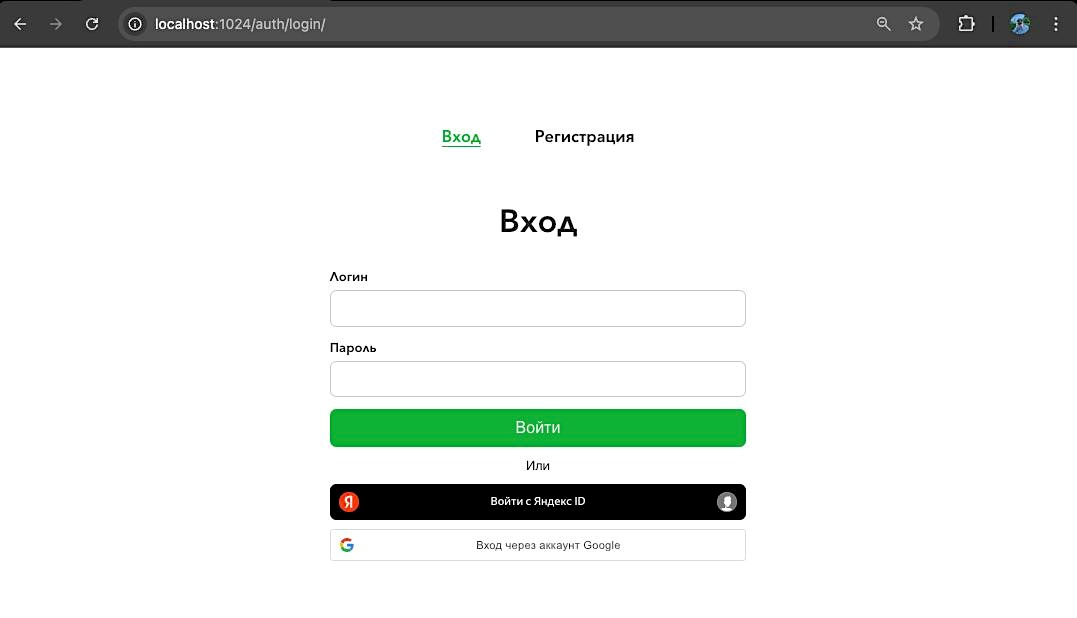
\includegraphics[width=1\linewidth]{images/loginPage.jpg}}
    \captionof{figure}{Страница авторизации}
    \label{fig:enter-label}
}

Рассмотрим каждый из них по очереди. Локальная авторизация - авторизация пользователей, которые сами зарегистрировались в системе с помощью внутренней формы регистрации, представленной на листинге 2.14.

\begin{lstlisting}[language=JavaScript, caption=Форма авторизации,breaklines=true]
1  <FormView displayName="login" action="edit">
2     <template #form-bottom="{ entity }">
3         <div class="form-bottom-column">
4             <BaseBtn @click="authorize(entity)">Войти</BaseBtn>
5             Или
6             <div id="auth-bottom"></div>
7             <div id="auth-bottom2"></div>
8         </div>
9     </template>
10 </FormView>
\end{lstlisting}

Рассмотрим форму авторимзации, представленную на листинге 2.14. На ней представлен компонент FomView у которого существует лишь 3 функциональные кнопки. Сама форма отображает всего 2 поля: поле ввода логина и поле ввода пароля с кнопками авторизации.

При нажатии на кнопку «Войти» срабатывает событие @click и вызвается функция authorize с параметром entity, полученный из формы. Реализация функции на листинге 2.15.

\begin{lstlisting}[language=JavaScript, caption=Метод авторизации пользователя,breaklines=true, ]
1 authorize(entity) {
2    this.$api.auth.login({ ...entity }, res => {
3        if (res?.detail) return
4        this.$ls.token = res.access_token
5        this.$ls.current_user = res.user_id
6        this.$store.commit('setUser', res.user_id)
7        this.$router.replace('/home')
8    })
9 },
\end{lstlisting}


Здесь вызывается API-метод авторизации login, которому передаются все значения из формы. Вторым параметром идет callBack - функция, выполняемая синхронно после успешного запроса. Она получает параметр res — ответ сервера, содержащий JWT-токен для доступа к приложению. Без этого токена дальнейшая работа с системой невозможна.

Вместе с токеном сервер возвращает уникальный идентификатор пользователя (userID), используемый для последующих запросов его данных на других страницах. Эти данные сохраняются в локальном хранилище браузера (localStorage) и во внутреннем состоянии приложения, чтобы обеспечить быстрый доступ при необходимости.

После успешной авторизации система перенаправляет пользователя на главную страницу, где инициализируется загрузка персональных данных и настройка интерфейса под его роль. Для защиты от несанкционированного доступа JWT-токен имеет ограниченный срок жизни (обычно 15–30 минут), а все запросы к API сопровождаются проверкой валидности подписи токена.

Авторизация через внешний сервис Яндекс.

OAuth требует предварительной регистрации приложения в системе разработчика Яндекса [39]. На этапе регистрации указывается список запрашиваемых данных пользователя (например, email, имя, аватар) и URL для перенаправления после успешного входа. Полученный ClientID (уникальный идентификатор приложения) сохраняется в конфигурации проекта и используется для формирования OAuth-запроса .

Для корректной работы необходимо строго соблюдать требования Яндекс.OAuth: callback URL должен точно соответствовать зарегистрированному, включая протокол (HTTP/HTTPS) и поддомены. Пример этих данных представлен на рисунке 32. 

\vspace{12pt}

{
    \centering
    \fbox{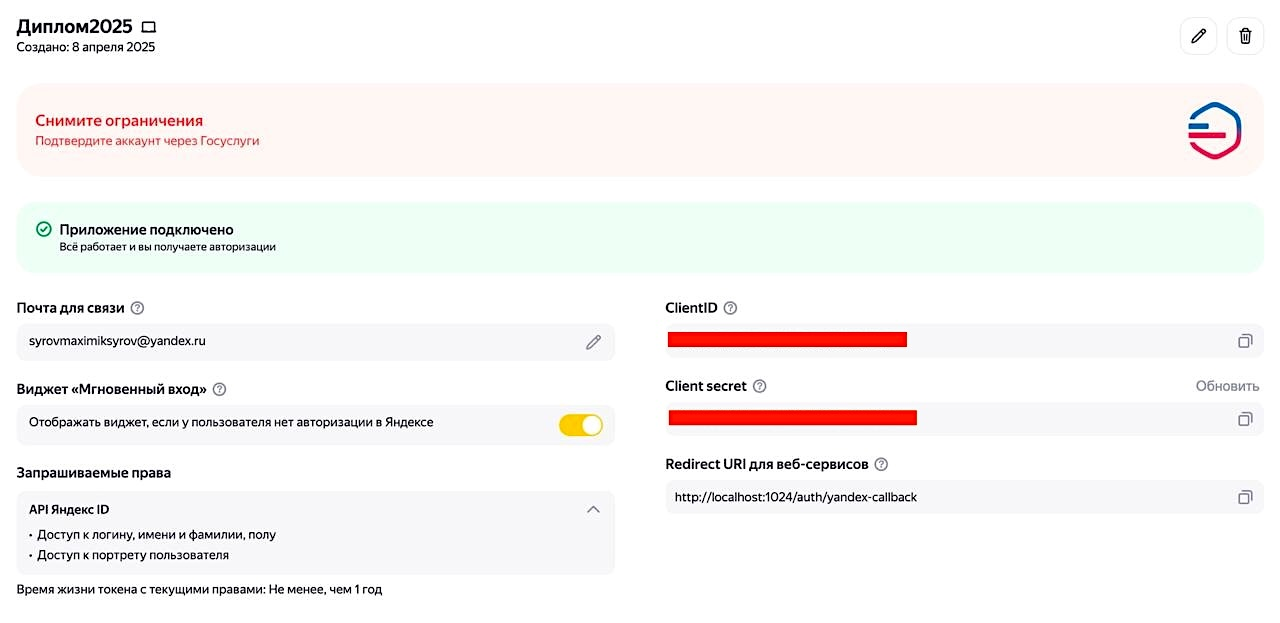
\includegraphics[width=0.9\linewidth]{images/2025-04-09 23.11.44.jpg}}
    \captionof{figure}{Страница с доступом приолжения в Яндекс Oauth}
    \label{fig:enter-label}
}

В финальной среде требуется дополнительная верификация домена через DNS-запись или загрузку файла-подтверждения. Клиентская часть должна обрабатывать ошибки перенаправления (например, отмену авторизации пользователем) и предусматривать fallback-механизм для повторного входа.

Механизм получения данных пользователя через Яндекс:
\begin{enumerate}
    \item Подключить кнопку авторизации в приложение (листинг В.4) при создании страницы авторизации Здесь подключается скрипт, предоставленный яндексом, который добавляет в DOM дерево свой компонент.
    \item Пользователь нажимает на неё, авторизуясь через свой аккаунт.
    \item С страницы на сервер яндекс отправляется запрос на получение токена доступа с помощью ClientID (листинг В.4, строки 7-13)
    \item После успешной авторизации пользователя, Яндекс перенаправляет пользователя на страницу, указанную в Личном кабинете авторизации и в запросе на получение токена (они обязательно должны совпадать) (листинг В.4, строка 12)
    \item Поскольку Яндекс открывает всплывающее окно, а не перенаправляет уже на открытую вкладку, получить токен на той же странице нельзя. Поэтому указана страница auth/yandex-callback, которая, получив токен доступа (листинг 2.16, строки 2 - 5), запрашивает у яндекса информацию о пользователе и сохраняет её в LocalStorage( листинг 2.16, строки 7, 8). После чего закрывает всплывающее окно (листинг 2.16, строка 9)
    \item На старой странице авторизации идет подписка на изменения в хранилище LocalStorage под ключом yandex\_user\_data (листинг 2.17). Таким образом, при изменении значения под этим ключом срабатывает функция, которая получает из LocalStorage данные, расшифровывает их и выполняет последовательно процесс регистрации, а затем авторизации.
\end{enumerate}
\begin{lstlisting}[language=JavaScript, caption=Получение данных о пользователе из Яндекса,breaklines=true]
1 mounted() {
2    const url = new URL(window.location.href)
3    const hash = url.hash.substring(1)
4    const params = new URLSearchParams(hash)
5    const accessToken = params.get('access_token')
6    if (!accessToken) return
7    this.$api.auth.yandexGetData(accessToken, 'json', data => {
8        this.$ls.setItemEncrypt('yandex_user_data', JSON.stringify(data))
9        window.close()
10    })
11 },
\end{lstlisting}
\begin{lstlisting}[language=JavaScript, caption=Регистрация и авторизация с данными полученные из Яндекса,breaklines=true]
1 this.$ls.subscribe('yandex_user_data', () => {
2    const userData = JSON.parse(this.$ls.getItemDecrypt('yandex_user_data'))
3    this.$api.auth.register(
4        {
5            name: userData.first_name,
6            \\ other data
7        },
8        () => {
9            this.authorize({
10               login: userData.login,
11               password: password,
12           })
13       }
14   )
15 })
\end{lstlisting}

Авторизация через внешний сервис Google. 

По аналогии с сервисом Яндекса, в Google Oauth необходимо зарегистрировать веб-приложение в их сервисе для управлениями авторизаций
[40] для получения данных о пользователях (рисунок 33).

\vspace{12pt}
{
    \centering
    \fbox{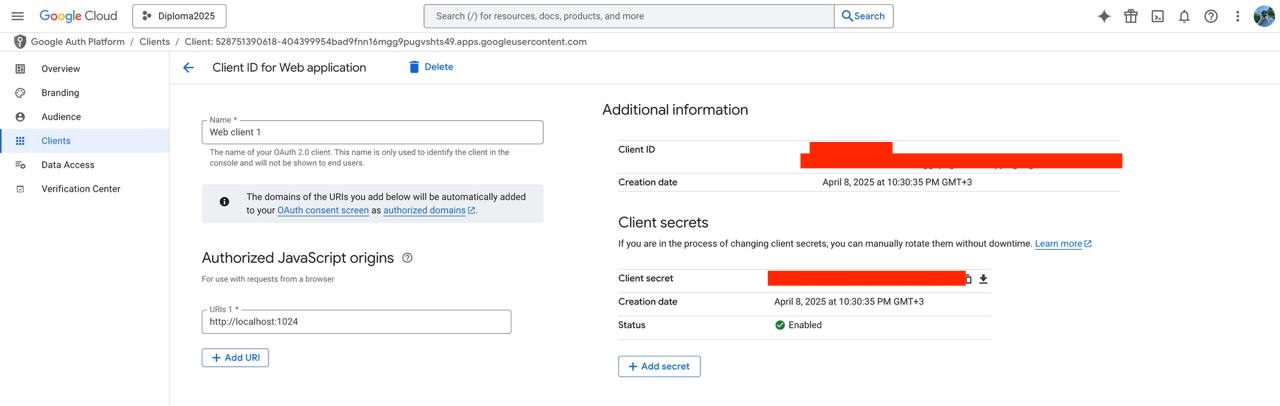
\includegraphics[width=1\linewidth]{images/2025-04-09 23.33.10.jpg}}
    \captionof{figure}{Страница с доступом приолжения в Google Oauth}
    \label{fig:enter-label}
}

Процесс авторизации пользователя через Google Oauth схож с методом Яндекса, но несколько проще.

Механизм получения данных пользователя через Google:
\begin{enumerate}
        \item Подключить кнопку авторизации в приложение (Приложение В Листинг В.5) при создании страницы авторизации. Здесь подключается скрипт, предоставленный google, который добавляет в DOM дерево свой компонент (листинг В.5, строка 2).
    \item Пользователь нажимает на неё, авторизуясь через свой аккаунт.
    \item После авторизации пользователем в сплывающем окне, отправляется запрос к серверам Google в котором указывается (листинг В.5, строки 6-24): client\_id - полученный ClientID при регистрации приложения, response\_type - то, что ожидается в результате запроса - token, те токен авторизации пользователя, scope - это политики доступа, callback - функция которая отработает в случае успешного запроса к Google.
    \item В случае успешного выполнения запроса, выполняется callback функция. В ней, одним из параметром является зашифрованный с помощью JWT - токен в credentials (листинг В.5, строки 7, 8), расшифровав который, можно получить данные пользователя.
    \item С помощью полученный данных пользователя, происходит регистрация и авторизация с помощью описанных ранее методов (Приложение В листинг В.5, строки 12 - 24).
        
\end{enumerate}

\section {Выводы по проектной части}

В второй главе подробно рассмотрена реализация веб приложения. Основное внимание уделено технической реализации серверной части, клиенской части, а также клиентского интерфейса. 
Разработка велась паралельно и одновременно для минимизации ошибок при стыкове серверной и клиентской части.

Серверная часть реализована с использованием Python и фреймворка FastAPI с использованием POSTful API взаимодействия с клиентом. Описано движение данных от клиента к серверу, к классам валидации и к бизнес логике. Описаны алгоритмы авторизизации а также взаимодействия с реляционной базой данных, которой было уделенно особое внимение - структуре данных, а также специальных запросов на получение информации об обучающихся и их занятий. Установлены все связи между таблицами, обеспечивающие корректность выборок и поддержку фильтрации.

Серверная часть реализована с помощью Vue.js - фрейморка над Java-\\Script. Описана структура клинетской части, описаны созданные моудли, такие как маршрутеризатор путей внутри приложения, API для отправки запросов на сервер, а также использование компонентного подхода внутри веб приложения.

В ходе второй главы была выполнена реализация всех ключевых компонентов веб-приложения. Система обеспечивает корректную работу пользовательского интерфейса, надежное взаимодействие с сервером и базой данных, поддержку сложных сценариев использования приложения для администрирования групповых занятий. Полученный результат является функционально завершенным и готовым к интеграции с дополнительными модулями.

\newpage
\chapter{ВНЕДРЕНИЕ И ЭКСПЛУАТАЦИЯ}
\section {Развертывание приложения}

Развертывание приложения происходит в 2 этапа. Первый этап - подготовка финальной сборки приложения к выпускаемой весрии. И второй этап - настройка доменного окружения и запуск приложения в сети интернет

Для успешного запуска эксплуатационной версии как клиентской, так и серверной части, а также базы данных независимо друг от друга, использован Docker [41].

Docker представляет собой платформу для контейнеризации приложений, обеспечивающую их изоляцию и воспроизводимость в различных средах выполнения. В рамках данной технологии ключевыми концепциями являются контейнеры, образы (images) и оркестрация, которые совместно решают проблему несоответствия сред разработки, тестирования и эксплуатации.

Контейнеры — это легковесные исполняемые среды, изолированные на уровне операционной системы. В отличие от виртуальных машин, они используют общее ядро ОС, что обеспечивает значительное снижение накладных расходов при запуске. Каждый контейнер инкапсулирует приложение со всеми его зависимостями (библиотеками, системными утилитами, конфигурациями), гарантируя идентичное поведение на любой платформе, поддерживающей Docker.

Образы служат шаблонами для создания контейнеров. Они формируются посредством многослойной сборки, где каждый слой соответствует конкретной инструкции в Dockerfile (например, установка пакетов, копирование файлов). Такой подход обеспечивает эффективное кэширование и повторное использование компонентов. Образы хранятся в реестрах, что упрощает их распространение и версионирование.

Практическая значимость Docker проявляется в следующих аспектах:

\begin{enumerate}
    \item Унификация сред: устранение расхождений между окружениями разработчиков, CI/CD-серверов и production-серверов.
    \item Масштабируемость: быстрое развертывание идентичных экземпляров приложения для обработки пиковых нагрузок.
    \item Микросервисная архитектура: изолированное функционирование компонентов системы с индивидуальными требованиями к окружению.
    \item Переносимость приложений: возможность быстрого развертывания готовых контейнеров между различными платформами и облачными провайдерами без изменения кода приложения.
\end{enumerate}



Для начала необходимо подготовить серверную часть сервиса.

В серверной части фигурирует 2 докер контейнера: один для запуска базы данных, другой для содержания всей бизнес логики сервиса.

За это отвечает Dockerfile, представленный в листинге 3.1.

\begin{lstlisting}[caption=Dockerfile серверной части]
1 FROM python:3.12
2 WORKDIR /app
3 COPY Pipfile Pipfile.lock /app/
4 COPY *.env /app/
5 RUN pip install pipenv
6 RUN pipenv install --ignore-pipfile
7 COPY ./app /app/
8 EXPOSE 8000
9 CMD ["pipenv", "run", "uvicorn", "main:app", "--host", "0.0.0.0", "--port", "8000"]
\end{lstlisting}

Здесь, сначала, на вход подается минимально допустимая версия питона, без которой серверная часть приложения не сможет скомпилироваться.

Далее переключаемся в рабочую директорию app внутри докер приложения. В этой директории располагаются все файлы, которым будет предоставлен ограниченный доступ через инетрент.

Далее в директорию копируются файлы Pipfile и Pipfile.lock - они описывают все необходимые библиотеки и зависимости для нормального функционирования серверной части приложения.

Далее происходит установка всех библиотек зависимостей.
И только потом с помощью демона uvicorn происходит запуск API на текущем хосте (локальном хосте) на 8000 порту. 
Теперь если пытаться обращаться к 8000 порту, то можно отправлять запросы к сервису.

Теперь рассмотрим запуск клиентской части приложения.

Поскольку сервис запускается в продакшн версии, использовать Node JS и встроенные скрипты для запуска приложения (npm run serve и прочее) не является возможным, поскольку такой способ подходит только для запуска в режиме разработки [42].
Соответственно, для функциональной работы мне понадобился самый простой функциональный сервис для запуска веб-сервера Nginx [43].

Nginx – это высокопроизводительный веб-сервер с открытым исходным кодом, который также может использоваться в качестве обратного прокси, кэширующего сервера и балансировщика нагрузки.

Конфигурация nginx представлена в файле nginx.conf и представлена на листинге 3.2.
\begin{lstlisting}[caption=Конфигурация Nginx]
1 server {
2    listen 1024;
3    server_name localhost;
4    location / {
5        root /usr/share/nginx/html;
6        index index.html;
7        try_files $uri $uri/ /index.html;
8        server_name m.syrov.ru www.m-syrov.ru;
9        add_header Cache-Control "no-cache, no-store, must-revalidate";
10       expires 0;
11   }
12   location /diploma {
13       proxy_pass http://89.104.71.146:8000;
14       proxy_set_header Host $host;
15       proxy_set_header X-Real-IP $remote_addr;
16       proxy_set_header X-Forwarded-For $proxy_add_x_forwarded_for;
17   }
18 }
\end{lstlisting}

Здесь Nginx выполняет простую функцию, позволяет получить доступ к статичным файлам веб приложения через обращение к 1024 порту.

Кроме этого, nginx проксирует все исходящие запросы клиентской части приложения от 1024 порта к 8000 порту, на котором запущено API, серверная часть приложения.

Для запуска nginx на виртуальной машине также понадобится docker с Docker файл с конфгурациями, представленные на листинге 3.3.

\begin{lstlisting}[caption=Dockerfile клиентской части]
1 FROM node:18 as builder
2
3 WORKDIR /app
4 COPY . .
\end{lstlisting}
\noindent Продолжение листинга 3.3
\vspace{13pt}
\begin{lstlisting}[captionpos=none, title={}]
5 FROM nginx:alpine as production
6 COPY --from=builder /app/dist /usr/share/nginx/html
7 COPY --from=builder /app/nginx.conf /etc/nginx/conf.d/default.conf
8 EXPOSE 1024
\end{lstlisting}

Здесь, происходит слудующее: docker копирует содержимое папки frontend к себе в общую папку app, откуда выполняет копирование nginx файлов конфигурации и выставления 1024 порта в обший доступ.


Предварительно, сделана build версия приложения через команду npm run build. Она использует встроенные методы Node js для оптимизации Vue файлов и компиляции их в нативный JavaScript код. Это нужно для из-за того, что браузеры умеют распознавать только нативный JavaScript код. При разработке браузер тоже читает нативный код [44], но ему предоставляются так называемые map карты по которым браузер может воссоздать первоначальный вид файлов до компиляции, предоставив разработчику средства для отладки кода)

Теперь, когда все докерфайлы готовы, можно собрать их и запустить их. 
За процесс сборки и запуска докер контейнеров в image файлы отвечает скрипт docker-compose.yml, представленный на листинге 3.4.

\begin{lstlisting}[caption=Скрипт docker-compose.yml]
1 version: '3.8'
2
3 services:
4  db:
5    image: postgres:latest
6    environment:
7      POSTGRES_USER: ${POSTGRES_USER}
8      POSTGRES_PASSWORD: ${POSTGRES_PASSWORD}
9      POSTGRES_DB: ${POSTGRES_DB}
10   ports:
11     - "5432:5432"
12   volumes:
13     - postgres_data:/var/lib/postgresql/data
14
15 backend:
15    image: backend:latest
16    restart: always
17    build:
18     context: ./backend
\end{lstlisting}
\noindent Продолжение листинга 3.4
\vspace{13pt}
\begin{lstlisting}[captionpos=none, title={}]
19      dockerfile: Dockerfile
20    ports:
21      - "8000:8000"
22    depends_on:
23      - db
24  frontend:
25    build: ./frontend
26    ports:
27      - "1024:1024"
28    depends_on:
29      - backend
30      - db
31 volumes:
32   postgres_data:
\end{lstlisting}


Здесь идет полное описание всех докер контейниров: db отвечает за базу данных, backend за серверную часть и frontend за клиентскую часть.

Теперь при запуске файла через команду `docker compose up --build` будет созданы и скомпилированы мои 3 контейнера и доступ к клиентской части приложения будет на 1024 порту.


Далее, рассмотрим процесс развертывания приложения в интернете.

Для публикации сервера в интернете, использован VPS [45].

VPS (Virtual Private Server) — это виртуальный выделенный сервер, представляющий собой изолированную среду на физическом сервере с гарантированными вычислительными ресурсами (CPU, RAM, дисковое пространство). В отличие от shared-хостинга, где ресурсы распределяются между множеством пользователей, VPS обеспечивает полный контроль над окружением за счет:

\begin{enumerate}
    \item Виртуализации на уровне ОС или аппаратной виртуализации, что позволяет устанавливать произвольное ПО и настраивать параметры ядра.
   \item Выделенных ресурсов, независимых от других пользователей.
   \item Root-доступа, обеспечивающего администрирование на уровне суперпользователя (установка серверного ПО, настройка брандмауэров, мониторинг).
\end{enumerate}

Виртуальные сервера позволяют запустить на них веб приложение, подключить к ним доменное имя [46] и иметь доступ к веб приложению через сеть интернет.

Проанализировав рынок поставщиков доменных услуг [47], был выбран рег.ру. Здесь было преобретено доменное имя m-syrov.ru на год за 130 рублей. Также, рег.ру предоставляет возможность приобрести VPS сервер за 540 рублей в месяц.

Получив доступы к своему VPS серверу и подключившись к нему по SSH, файлы проекта были перенесены, запустил docker-compose, описанный выше, и открыл своей сервис в открытый доступ[48].

\section {Проведение тестирования сервиса}

Для проведения успешного тестирования созданного сервиса были созданы слудеющие сценарии тестирования и тест кейсы.

Тест-кейс [49] – это документированный набор шагов, условий и ожидаемых результатов, предназначенный для проверки конкретной функциональности или сценария работы программного обеспечения. Тест-кейс помогает систематизировать процесс тестирования и обеспечивает воспроизводимость проверок.

Сценарное тестирование [50] – это метод тестирования, при котором проверяется работоспособность системы в условиях, максимально приближенных к реальному использованию. 

Оно основывается на пользовательских сценариях (например, «регистрация нового ученика и запись его на занятие») и оценивает, как приложение ведет себя в комплексных ситуациях, а не только при изолированных проверках отдельных функций.


Тест создания открытой группы.

Шаги воспроизведения:
\begin{enumerate}
    \item Зарегистрировать нового пользователя с ролью учителя и авторизоваться.
    \item Нажать на кнопку создание группы.
    \item Ввести правильные данны в поля формы.
    \item Нажать кнопку «Сохранить».
\end{enumerate}

Ожидаемым результатом теста является создание новой группы и событие редиректа на карточку созданной группы.

Фактический результат - тест выполнен.

Тест вступления в группу и авторизации через сторонний сервис.

Шаги воспроизведения:
\begin{enumerate}
    \item Авторизоваться через Яндекс.
    \item Открыть список групп.
    \item Выбрать фильтр по чужим открытым группам.
    \item Выбрать группу и нажать кнопку «Вступить».
\end{enumerate}

Ожидаемый результат:
\begin{enumerate}
    \item В карточке группы на вкладке участников есть имя авторизованного пользователя.
    \item В расписании есть занятия группы, в которую вступил пользователь.
\end{enumerate}

Фактический результат - тест выполнен.

Тест принятия пользователя в закрытую группу.

Шаги воспроизведения:

\begin{enumerate}
    \item Авторизоваться за пользователя с ролью обучающегося.
    \item Перейти в список групп и выбрать фильтр по закрытым группам.
    \item Выбрать группу и нажать кнопку «Отправить запрос».
    \item Выйти из аккаунта.
    \item Авторизоваться за пользователя с ролью преподавателя.
    \item Перейти в карточку своей закрытой группы.
    \item В списке запросов на вступление выбрать заявку от ученика.
    \item Нажать кнопку «Принять».
\end{enumerate}

Ожидаемым результатом теста является:

\begin{enumerate}
    \item Ученик должен перенестись в список участников группы.
    \item Ученик должен увидеть себя в списке участников этой закрытой группы.
\end{enumerate}

Фактический результат - тест выполнен.

Тест создания занятий без привязки к группе.

Шаги воспроизведения:
\begin{enumerate}
    \item Авторизоваться за пользователя с ролью преподавателя.
    \item Перейти в расписание.
    \item Нажать кнопку «Добавить слот».
    \item Заполнить правильные данные в форме, сохранить.
\end{enumerate}

Ожидаемым результатом теста является видимость слота в расписании преподавателя, а также в разделе мои слоты в карточке пользователя.

Фактический результат - тест выполнен.

Тест изменения успеваемости обучающихся в слоте.

Шаги воспроизведения:
\begin{enumerate}
    \item Авторизоваться за пользователя с ролью преподавателя.
    \item Перейти в расписание.
    \item Нажать кнопку «Добавить слот».
    \item Заполнить правильные данные в форме, сохранить.
    \item Авторизоваться за пользователя с ролью обучающегося.
    \item Перейти в расписание, открыть расписание слотов преподавателя путем поиска его слотов в фильтре расписания.
    \item Найти слот и забронировать место в нем.
    \item Авторизоваться за пользователя с ролью преподавателя.
    \item Открыть карточку слота, перейти в раздел участников.
    \item Нажать на галочку в столбце успеваемость обучаемого.
    
\end{enumerate}

Ожидаемый результат теста является сохранение успеваемости при обновлении страницы.

Фактический результат - тест выполнен.



\section {Анализ возможностей развития приложения}

Работа над веб приложением продолжается. Развитие приложения предполагается проводить по нескольким направлениям: функциональность, производительность, внешний вид, монетизируемость.

С точки зрения нового функционала, основной упор будет сделан на достижение большего удобства пользователя и увеличения продуктивности во время использоваения приложения. Самое приоритеное исправление - поиск и своевременное исправление возникающих ошибок отображения форм, таблиц и фильтров. Для этого планируется создание окружения автоматического компонентного, а также сценарного тестирования. 

Следующим по приоритету стоит новый функционал. В будущих обновлениях планируется добавление возможности добавлять изображения к группам, а также просматривать группы в виде плиток. Это уменьшит когнитивную нагрузку пользователя и заставит меньше вчитываться в описания групп и позволит добавить большей индивидуальности группам. Дополнительно будет реализована интеллектуальная система рекомендаций групп на основе анализа предпочтений пользователя и его активности в приложении.

Далее планируется функционал синхронизации расписания с встроенными календарями мобильных устройств на платформах Android и iOS. Это позволит пользователям не терять свои предстоящие занятия.

Следующей приоритеной задачей будет добавление разделов аналитики и статистики. Необходимо будет дать информацию преподавателям об успеваемости по каждой группе, а также статистические данные по заработкам за предыдущие периоды, а также сформирование тренда на будущий заработок.
Для обучающихся же, разделы статистики будут полезны для понимания своей успеваемости как по отдельным предметам, так и за отдельные периоды.
Это позволит пользователям лучше понимать свое расписание и вносить корректировки в своё обучение.

Для повышения производительности приложения, первым делом, необходимо будет расширить вычислительные возможности VPS сервера, на котором развернуто веб приложение. Планируемое улучшение сервиса должно включать в себя как минимум 16Гб оперативной памяти, 4-х ядерный процессор с средней частотой 2.5Ггц, а также порядка 500Гб встроенной памяти.

Данное расширение позволит увеличить пропускную способность сервиса с 100 до 1000 пользоателей, одновременно использующих сайт.

Также, для увеличения производительности, следует выделить время на проведение рефакторинга отдельных модулей и функций для уменьшения комплексности алгоритмов, а также ускорению работы сервиса.

Следующим важным шагом для увеличения производительности станет добавление нового типа базы данных Redis [51]. Redis позволяет хранить данные не на жестком диске виртуальной машины, а напрямую в оперативной памяти. Это позволит ускорить самые частые запросы к базе данных и сократить время ожидания пользователей под нагрузкой. Однако redis имеет ряд недостатков. Во первых, при выключении работы сервиса, все данные в оперативной памяти будут очищены. Также, оперативная память существенно меньше чем память жесткого диска, поэтому она будет полезна только для постоянно изменяемых данных, долгое хранение которых не имеет смысла.

Redis будет идеален для временного хранения истекщих токенов доступа пользователей. Поскольку время жизни каждого токена доступа составляет всего 30 минут по умолчанию, ежедневное очищение этой таблицы не приведет к потере каких-либо важных данных, а только ускорит работу сервиса, потому что при каждом запросе к любому ендпоинту происходит как минимум 1 обращение к этой таблице.

Для поддержания актуальности внешнего вида веб-сайта будет продолжена работа над улучшением и изменениями стилей и внешнего вида различных компонентов внутри приложения.

Самым крупным из таких обновлений будет продолжена работа над созданием аддаптивной версии веб сайта под устройства с узким экраном, а в дальнейшем полный аддаптив под мобильные устройства. Это улучшение позволит пользователям открывать  с мобильных устройств.

Для финансирования всех вышеперечисленных нововведений, необходима частичная монетизация сервиса. Планируется, что основной функционал останется бесплатным, однако, часть функционала, который заточен на использование основных мощностей и большого количества пользователей - будет платным.
В платном плане - создание неограниченного количества групп (фактически до 250 групп), в бесплатном плане до 30 групп.

Максимальное количество участников одной группы 30 человек -  в бесплатном плане, до 150 человек в платном плане.

Максимальное количество участников внутри занятия будет также ограничено 30 пользователями в бесплатном плане и 150 в платном.

В бесплатном плане планируется добавить по одному рекламному банеру на каждую старницу приложения. В платном плане рекламы не будет.

Итак, рассчет стоиости плана будет зависеть от среднего количества пользователей постоянно испольующих сервис, а также от стоиости одного просмотра и клика по рекламному банеру. 

Для расчета средней стоимости месячной подписки сервиса можно использовать следующую усовершенствованную формулу (1), которая учитывает как затраты, так и потенциальный доход от рекламы:
{\setlength{\abovedisplayskip}{0pt} % Отступ сверху
 \setlength{\belowdisplayskip}{0pt} % Отступ снизу
\begin{align}
S = (M + F) - (A \times C \times (V \times P_v + K \times P_k)),
\end{align}
}
где \(S\) - итоговая стоимость подписки для пользователя (руб/мес); \\ 
\(M\) - затраты на хостинг и VPS (руб/мес);\\
\(F\) - фиксированная зарплата разработчику;\\
\(A\) - среднее количество показов рекламы на пользователя в день;\\
\(C\) - количество активных пользователей;\\
\(V\) - CTR (click-through rate) - процент кликов по рекламе;\\
\(P_v\) - доход за 1000 показов (RPM) в рублях;\\
\(K\) - конверсия в клики (например, 0.5\% = 0.005);\\
\(P_k\) - доход за клик в рублях.

С помощью формулы (1) приведем предварительные расчеты. Предположим, что постоянные затраты (\(M\), \(F\)) = 50,000 руб/мес и имеем 1,000 активных пользователей (\(C\)).

Также, условно считаем, что имеем 5 показов рекламы на пользователя в день (\(A\)).

30 дней в месяце, то есть 5 \(\times\) 30 = 150 показов на одного пользователя в месяц. Сдедовательно:

RPM (\(P_v\)) = 50 руб за 1000 показов, те 0.05 руб за показ.

CTR (\(V\)) = 2\% те 0.02.

Доход за клик (\(P_k\)) = 5 (руб.)

Расчет дохода от рекламы достежим с помощью формулы 2.
{\setlength{\abovedisplayskip}{0pt} % Отступ сверху
 \setlength{\belowdisplayskip}{0pt} % Отступ снизу
\begin{align}
S &= C \times (A \times 30) \times (P_v + V \times P_k) 
\end{align}
}

Согласно формуле (2) рассчитаем доход от рекламы:

1000 \(\times\) 150 \(\times\) (0.05 + 0.10) = 

= 1000 \(\times\) 150 \(\times\) 0.15 = 22 500  (руб.)

Итоговая стоимость подписки:

S = 50,000 - 22,500 = 27,500 (руб.)

Распределение на пользователей:

Если 10 \% пользователей платные: 100 платных пользователей.

27,500 / 100 = 275 (руб/мес) за одну подписку.



\section {Выводы по внедрению и эксплуатации}

В результате выполнения третьей главы была достигнута основная цель по развертыванию приложения - разработаны и детально описаны схемы запуска, обеспечивающие стабильную работу системы в глобальной сети Интернет. В ходе работы реализовано полнофункциональное веб-приложение, размещенное на выделенном доменном имени с настроенной SSL-защитой.

Особое внимание уделено комплексному тестированию, включающему проверку ключевых сценариев использования, нагрузочное тестирование, аудит безопасности и оценку удобства интерфейса. Это позволило достичь высокой степени завершенности проекта: все запланированные функции реализованы в полном объеме, техническая часть обеспечивает стабильность работы даже при пиковых нагрузках, а система защиты данных соответствует современным стандартам.

Помимо готового к промышленной эксплуатации решения, проанализированы перспективы развития по нескольким направлениям. С функциональной точки зрения запланирована интеграция с дополнительными сервисами через API. Для повышения производительности подготовлена дорожная карта оптимизации работы с большими массивами данных. В части пользовательского интерфейса определены приоритеты по модернизации в соответствии с актуальными трендами UX/UI-дизайна. Отдельное внимание уделено вопросам монетизации, включая внедрение платного функционала и партнерских программ, что обеспечит устойчивое развитие проекта в долгосрочной перспективе.

\chapter*{ЗАКЛЮЧЕНИЕ}
\addcontentsline{toc}{chapter}{ЗАКЛЮЧЕНИЕ}

В ходе выполнения выпускной квалификационной работы была разработана специализированная веб-платформа для администрирования групповых занятий, направленная на решение ключевых проблем частных преподавателей и малых образовательных проектов. В рамках исследования проведен анализ предметной области, целевой аудитории и конкурентных решений, что позволило сформулировать требования к системе и спроектировать оптимальную архитектуру приложения.

Реализация платформы включала разработку серверной части на Python (FastAPI) с RESTful API, клиентского интерфейса на Vue.js и реляционной базы данных с продуманной структурой для эффективного управления учебными процессами. Тестирование подтвердило корректность работы всех модулей, включая автоматизацию расписаний, учет посещаемости и платежей, а также управление группами обучающихся.

Дальнейшее развитие проекта предполагает:

\begin{enumerate}
    \item Расширение функционала: интеграция с платежными системами, добавление мобильного приложения, внедрение аналитики успеваемости.
    \item Оптимизацию производительности: масштабирование серверной части, кэширование данных, улучшение отзывчивости интерфейса.
    \item Коммерциализацию: запуск пилотного внедрения в локальных образовательных проектах, разработка монетизации (подписка, премиум-функции).
    \item Масштабирование: адаптацию платформы для корпоративного обучения и дополнительных рынков.
\end{enumerate}


Полученные результаты демонстрируют готовность решения к практическому применению, а намеченные направления развития открывают перспективы для превращения проекта в полноценный коммерческий продукт.

\newpage
\chapter*{СПИСОК ЛИТЕРАТУРЫ}
\addcontentsline{toc}{chapter}{СПИСОК ЛИТЕРАТУРЫ}

\begin{enumerate}
    \item Карлов, И. А. Анализ цифровых образовательных ресурсов и сервисов для организации учебного процесса школ / И. А. Карлов и др. ; Нац. исслед. ун-т «Высшая школа экономики», Ин-т образования. – М. : НИУ ВШЭ, 2020. – 72 с. – ISSN 2500-0608. - Текст: электронный.
    \item Коблова, М. В. Использование электронной системы обучения в образовательном процессе / М. В. Коблова // Компьютерные науки и информационные технологии : материалы Междунар. науч. конф., Саратов, 01–04 июля 2020 г. / отв. ред. В. А. Твердохлебов ; отв. за вып. Т. В. Семенова, А. Г. Федорова. – Саратов : ИЦ «Наука», 2020. – С. 139–141  - Текст: электронный.
    \item Саидова, К. З. Анализ деятельности репетиторов / К. З. Саидова, Г. Р. Пожидаев, И. Д. Котилевец, И. А. Иванова // Информатика и образование. 2021. – Т. 36, № 6. – С. 18–28. – ISSN 0234-0453. - Текст: электронный.
    \item Баланов, А. Н. Прототипирование и разработка пользовательского интерфейса: оптимизация UX : учеб. пособие для вузов / А. Н. Баланов. – СПб. : Лань, 2024. – 220 с. – ISBN 978-5-507-49211-4. - Текст: электронный..
    \item  Клименко, И. С. Управление в организационных системах: учебное пособие для вузов / И. С. Клименко, Е. А. Палкин. — 2-е изд., стер. — Санкт-Петербург: Лань, 2025. — 324 с. — ISBN 978-5-507-52214-9. — Текст: электронный // Лань: электронно-библиотечная система. - Текст: электронный. 
    \item  ЯРепетитор [Электронный ресурс]. — URL: https://web.yarepetitor.\\com/auth (дата обращения: 16.02.2025). 
    \item Гутгарц, Р. Д. О формализации функциональных требований в проектах создания информационных систем / Р. Д. Гутгарц,Е. И. Провилков // Программные продукты и системы. – 2021. – № 3. – С. 349–357. – EDN GXHPFX.  - Текст: электронный.
    \item ГОСТ Р 50.1.028-2001. Информационные технологии поддержки жизненного цикла продукции. Методология функционального моделирования. - Текст: электронный.
    \item Работа веб-приложения: особенности, отличия от сайта и виды [Электронный ресурс]. – URL: https://skyeng.ru/magazine/wiki/it-industriya/chto-takoe-veb-prilozhenie/ (дата обращения: 16.02.2025).
    \item Дронов, В. А. HTML 5, CSS 3 и Web 3.0. Разработка современных Web-сайтов./ В. А. Дронов // СПб.: БХВ-Петербург, 2020. — 416 с. ISBN 978-5-9775-0596-3 - Текст: электронный.
    \item McFedries, P. HTML, CSS, \& JavaScript® All-in-One For Dummies / P. McFedries // WILEY \& SONS, INCORPORATED - Канада, 2023 - 848 с. ISBN: 978-1-394-16468-4 - Текст: электронный.
    \item  ECMAScript® 2025 Language Specification [Электронный ресурс].- URL: https://tc39.es/ecma262/ (дата обращения: 01.03.2025).
    \item Method Definitions [Электронный ресурс]. – URL: https://clck.ru/\\3MEizV (дата обращения: 02.03.2025).
    \item Джуба, С. Изучаем PostgreSQL 10 / С. Джуба, А. Волков // пер. с анг. А. А. Слинкина. – М.: ДМК Пресс, 2021. – 400 с. ISBN 978-5-97060-643-8 - Текст: электронный.
    \item  SQL/JSON standard-2020 conformance for PostgreSQL, Oracle, SQL Server and MySQL [Электронный ресурс]. - URL: https://obartunov.livejournal.\\com/200076.html (дата обращения: 04.03.2025).
    \item  Урванова, Е. С. Какую систему управления базами данных с открытым исходным кодом выбрать для проекта / Е. С. Урванова // Студенческий. – 2024. – № 21-2(275). – С. 47-49.  — Текст: электронный // Elibrary: электронно-библиотечная система.
    \item Silberschatz, A. Database System Concepts / H. Korth, S. Sudarshan- 4th ed. – New York : McGraw-Hill, 2022. – Section 4.10.2: Join Types and Conditions.– p. 166. – ISBN 0072283637 - Текст: электронный.
    \item TIOBE Index for April 2025 [Электронный ресурс]. – URL: https://ww\\w.tiobe.com/tiobe-index/ (дата обращения: 01.04.2025).
    \item FastAPI Documentation [Электролнный ресурс]. - URL: https://fastapi.\\tiangolo.com/ (дата обращения: 01.04.2025).
    \item MVC XEROX PARC 1978–79 [Электронный ресурс]. - URL: https://w\\ayback.archive-it.org/10370/20180425071111/http://folk.uio.no/trygver/themes/m\\vc/mvc-index.html (дата обращения: 05.04.2025).
    \item RFC 7231 — Hypertext Transfer Protocol (HTTP/1.1): Semantics and Content / Fielding, R., Reschke, J. [Электронный ресурс]. – URL: https://clck.ru/\\3MEj6C (дата обращения: 06.04.2025).
    \item Martin, J. Managing the Data-base Environment. – Englewood Cliffs, N.J. : Prentice-Hall, 2010. – 381 p. – ISBN 0-135-50582-8 - Текст: электронный..
    \item Особенноcти формирования моделей и построение базы данных в бизнесе на платформе Django ORM / М. Б. Тлебаев и др. // Вестник Кыргыз. Гос. Ун-та им. И. Арабаева. – 2023. – № 2. – С. 299–309. – DOI 10.33514/1694-7851-2023-2-299-309 - Текст: электронный.
    \item  The Python SQL Toolkit and Object Relational Mapper [Интернет ресурс]. - URL: https://www.sqlalchemy.org/ (дата обращения: 22.03.2025).
    \item  Documentation for Pydentic [Интернет ресурс]. - URL: https://docs.\\pydantic.dev/latest/ (дата обращения: 23.03.2025).
    \item  Репозиторий проекта [Сайт]. - URL: https://github.com/moximilian/Di\\ploma (дата обращения: 02.01.2025).
    \item RFC 7231 — Hypertext Transfer Protocol (HTTP/1.1): Semantics and Content / Fielding, R., Reschke, J. [Электронный ресурс]. – URL: https://clck.ru/\\3MEj6C (дата обращения: 06.04.2025).
    \item Martin, J. Managing the Data-base Environment. – Englewood Cliffs, N.J. : Prentice-Hall, 2020. – 381 p. – ISBN 0-135-50582-8.
    \item Мухортов, В. В. Объектно-ориентированное программирование, реализация и дизайн : метод. пособие / В. В. Мухортов, В. Ю. Рылов.– Новосибирск : ООО «Новософт», 2022. – 108 с.
    \item Пилькевич, П. В. Способы улучшения защищённости сервисов, использующих JWT-токены / П. В. Пилькевич // Сб. материалов I Молодежной науч.-практ. Конф., Севастополь, 08 февр. 2023 г. – Севастополь : СевГУ, 2023. – С. 96–97.  - Текст: электронный.
    \item Старанцова, Е. В. Методы хеширования паролей / Е. В. Старанцова// Пути инновационного развития науки и образования в современных условиях : сб. науч. Тр. – Миасс : Изд-во «Аниго», 2023. – С. 387–394. - Текст: электронный.
    \item Веселова, С. В. Цифровая обработка изображений : учеб. пособие / С. В. Веселова, Е. В. Константинова, И. В. Александрова. – СПб. : СПбГИКиТ, 2021. – 283 с. – ISBN 978-5-94760-493-1. - Текст: электронный.
    \newpage
    \item Дьяков, А. Г. Javascript для создания веб-приложений / А. Г. Дьяков, А. Н. Шмелева // Уральский научный вестник.– 2022.– Т. 10, № 2. – С.70–74.- Текст: электронный.
    \item Еремин, М. В. Сравнительный анализ популярных JavaScript фронтенд решений / М. В. Еремин // Тенденции развития науки и образования. – 2022. – № 87-1. – С. 64–68. – DOI 10.18411/trnio-07-2022-14. - Текст: электронный.
    \item Механизмы отрисовки. Документация Vue [Электронный ресурс]. - URL: https://ru.vuejs.org/guide/extras/rendering-mechanism.html (дата обращения: 02.04.2025).
    \item Навигация. Маршрутеризация. Документация Vue.js [Электронный ресурс]. – URL: https://vue-router-ru.netlify.app/guide/ (дата обращения: 02.04.\\2025).
    \item Fetch API. Сетевые запросы [Электронный ресурс]. - URL: https://lea\\rn.javascript.ru/fetch-api (дата обращения: 12.04.2025).
    \item Реактивность. Документация Vue.js [Электронный ресурс]. - URL: https://clck.ru/3MEjFf (дата обращения: 02.04.2025).
    \item Авторизация через учетную запись Yandex [Сайт]. - URL: https://oaut\\h.yandex.ru/client (дата обращения: 24.04.2025).
    \item Авторизация через учетную запись Google [Сайт]. - URL: https://con\\sole.cloud.google.com/ (дата обращения: 24.04.2025).
    \item  Сейерс, Э. Х. Docker на практике / Э. Х. Сейерс, А. Милл - 1-е изд. - Москва: Manning, 2024 - 516 с. - ISBN: 978-5-97060-772-5 - Текст: электронный.
    \item Круглик, Р. И. Использование инструмента Webpack для сборки веб-приложений / Р. И. Круглик // Постулат. – 2020. – № 1(51). – С. 52. - Текст: электронный.
    \item Основная функциональность HTTP сервера Nginx [Электронный ресурс]. – URL: https://nginx.org/ru/ (дата обращения: 03.05.2025).
    \item Механизмы рендера Vue компонентов. Документация Vue.js [Электронный ресурс]. - URL: https://clck.ru/3MEjJN (дата обращения: 12.03.2025).
    \item Габдуллин, И. И. Сравнение VDS/VPS серверов с виртуальным хостингом и физическим выделенным сервером / И. И. Габдуллин, И. А. Кожевникова // Достижения и приложения современной информатики, математики и физики : материалы IX Всерос. науч.-практ. конф., Нефтекамск, 29 нояб. 2021 г. – Уфа : БашГУ, 2021. – С. 39–42. - Текст: электронный.
    \item Что такое DNS простыми словами [Электронный ресурс]. - URL: https://clck.ru/3MEjMo (дата обращения: 06.05.2025).
    \item Обзор зарубежных и российских регистраторов доменных имён [Электронный ресурс]. – URL: https://habr.com/ru/articles/338206/ (дата обращения: 28.04.2025).
    \item Веб приложение администрирования групповых занятий [Сайт]. - URL: http://m-syrov.ru:1024/auth/login (дата обращения: 07.05.2025).
    \item Александрова, Е. Г. Свойства качественных тест-кейсов / Е. Г. Александрова, Н. Н. Добрынина // Современные технологии и научно-технический прогресс. – 2024. – № 11. – С. 107–108.
    \item Денисенко, А. В. Тестирование веб-приложений: автоматизация против ручного тестирования / А. В. Денисенко // Цифровая трансформация: вчера, сегодня, завтра : Материалы научно-технологической конференции, посвященной юбилею кафедры цифровых и аддитивных технологий СПбГУПТД, Санкт-Петербург, 09 октября 2024 года. – Санкт-Петербург: Санкт-Петербургский государственный университет промышленных технологий и дизайна, 2025. – С. 196-199.
   \item Архипкин, В. М. Повышение скорости работы информационных систем с использованием Redis / В. М. Архипкин // Информационные технологии в процессе подготовки современного специалиста : межвуз. сб. науч. тр. – Липецк : ЛГПУ им. П. П. Семенова-Тян-Шанского, 2024. – С. 30–35.
\end{enumerate}

\newpage
\addcontentsline{toc}{chapter}{ПРИЛОЖЕНИЕ А}

\includepdf[pages=-, scale=1]{parts/ТЗ.pdf} 

\chapter*{ПРИЛОЖЕНИЕ Б}

\addcontentsline{toc}{chapter}{ПРИЛОЖЕНИЕ Б}

\section*{Б.1 UML диаграмма по пользователям}

\renewcommand{\thefigure}{Б.\arabic{figure}}

{
    \centering
    \fbox{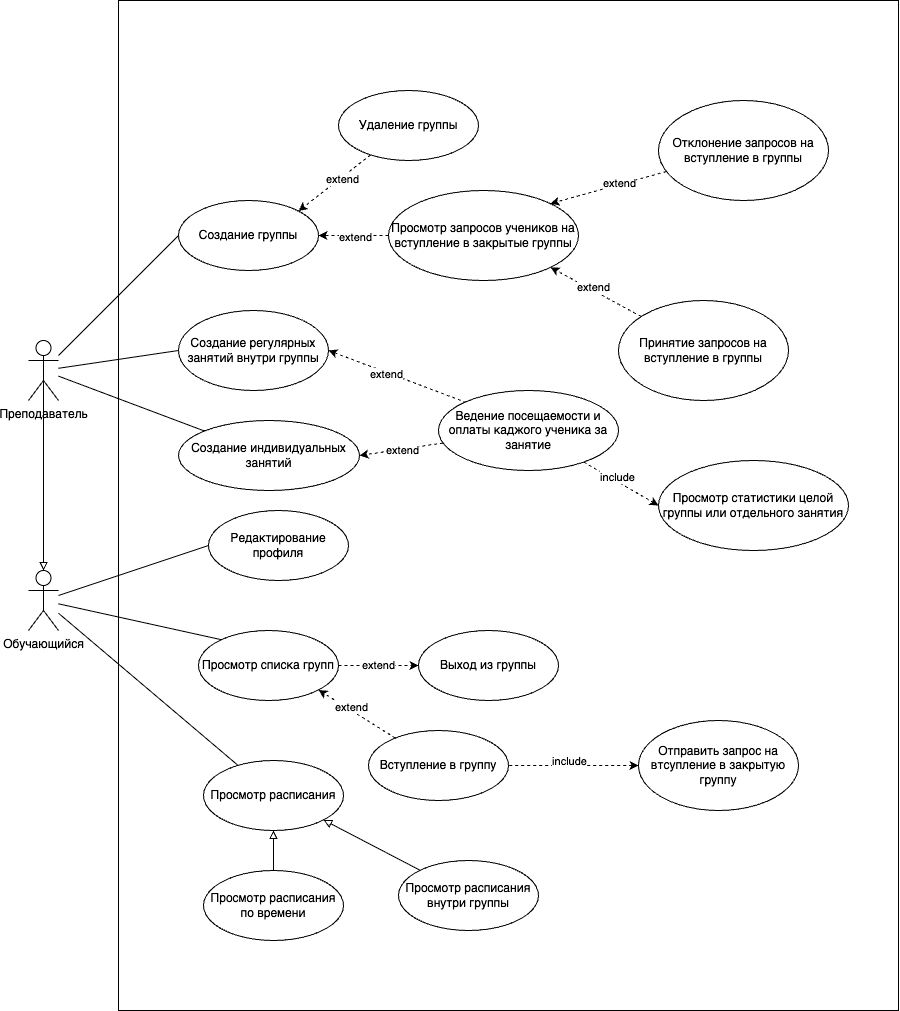
\includegraphics[width=1\linewidth]{images/UML.png}}
    % \captionof{figure}{UML диаграмма по пользователям}
}

\section*{Б.2 Прототип страницы «Расписание». Календарь, день}

{
    \centering
    \fbox{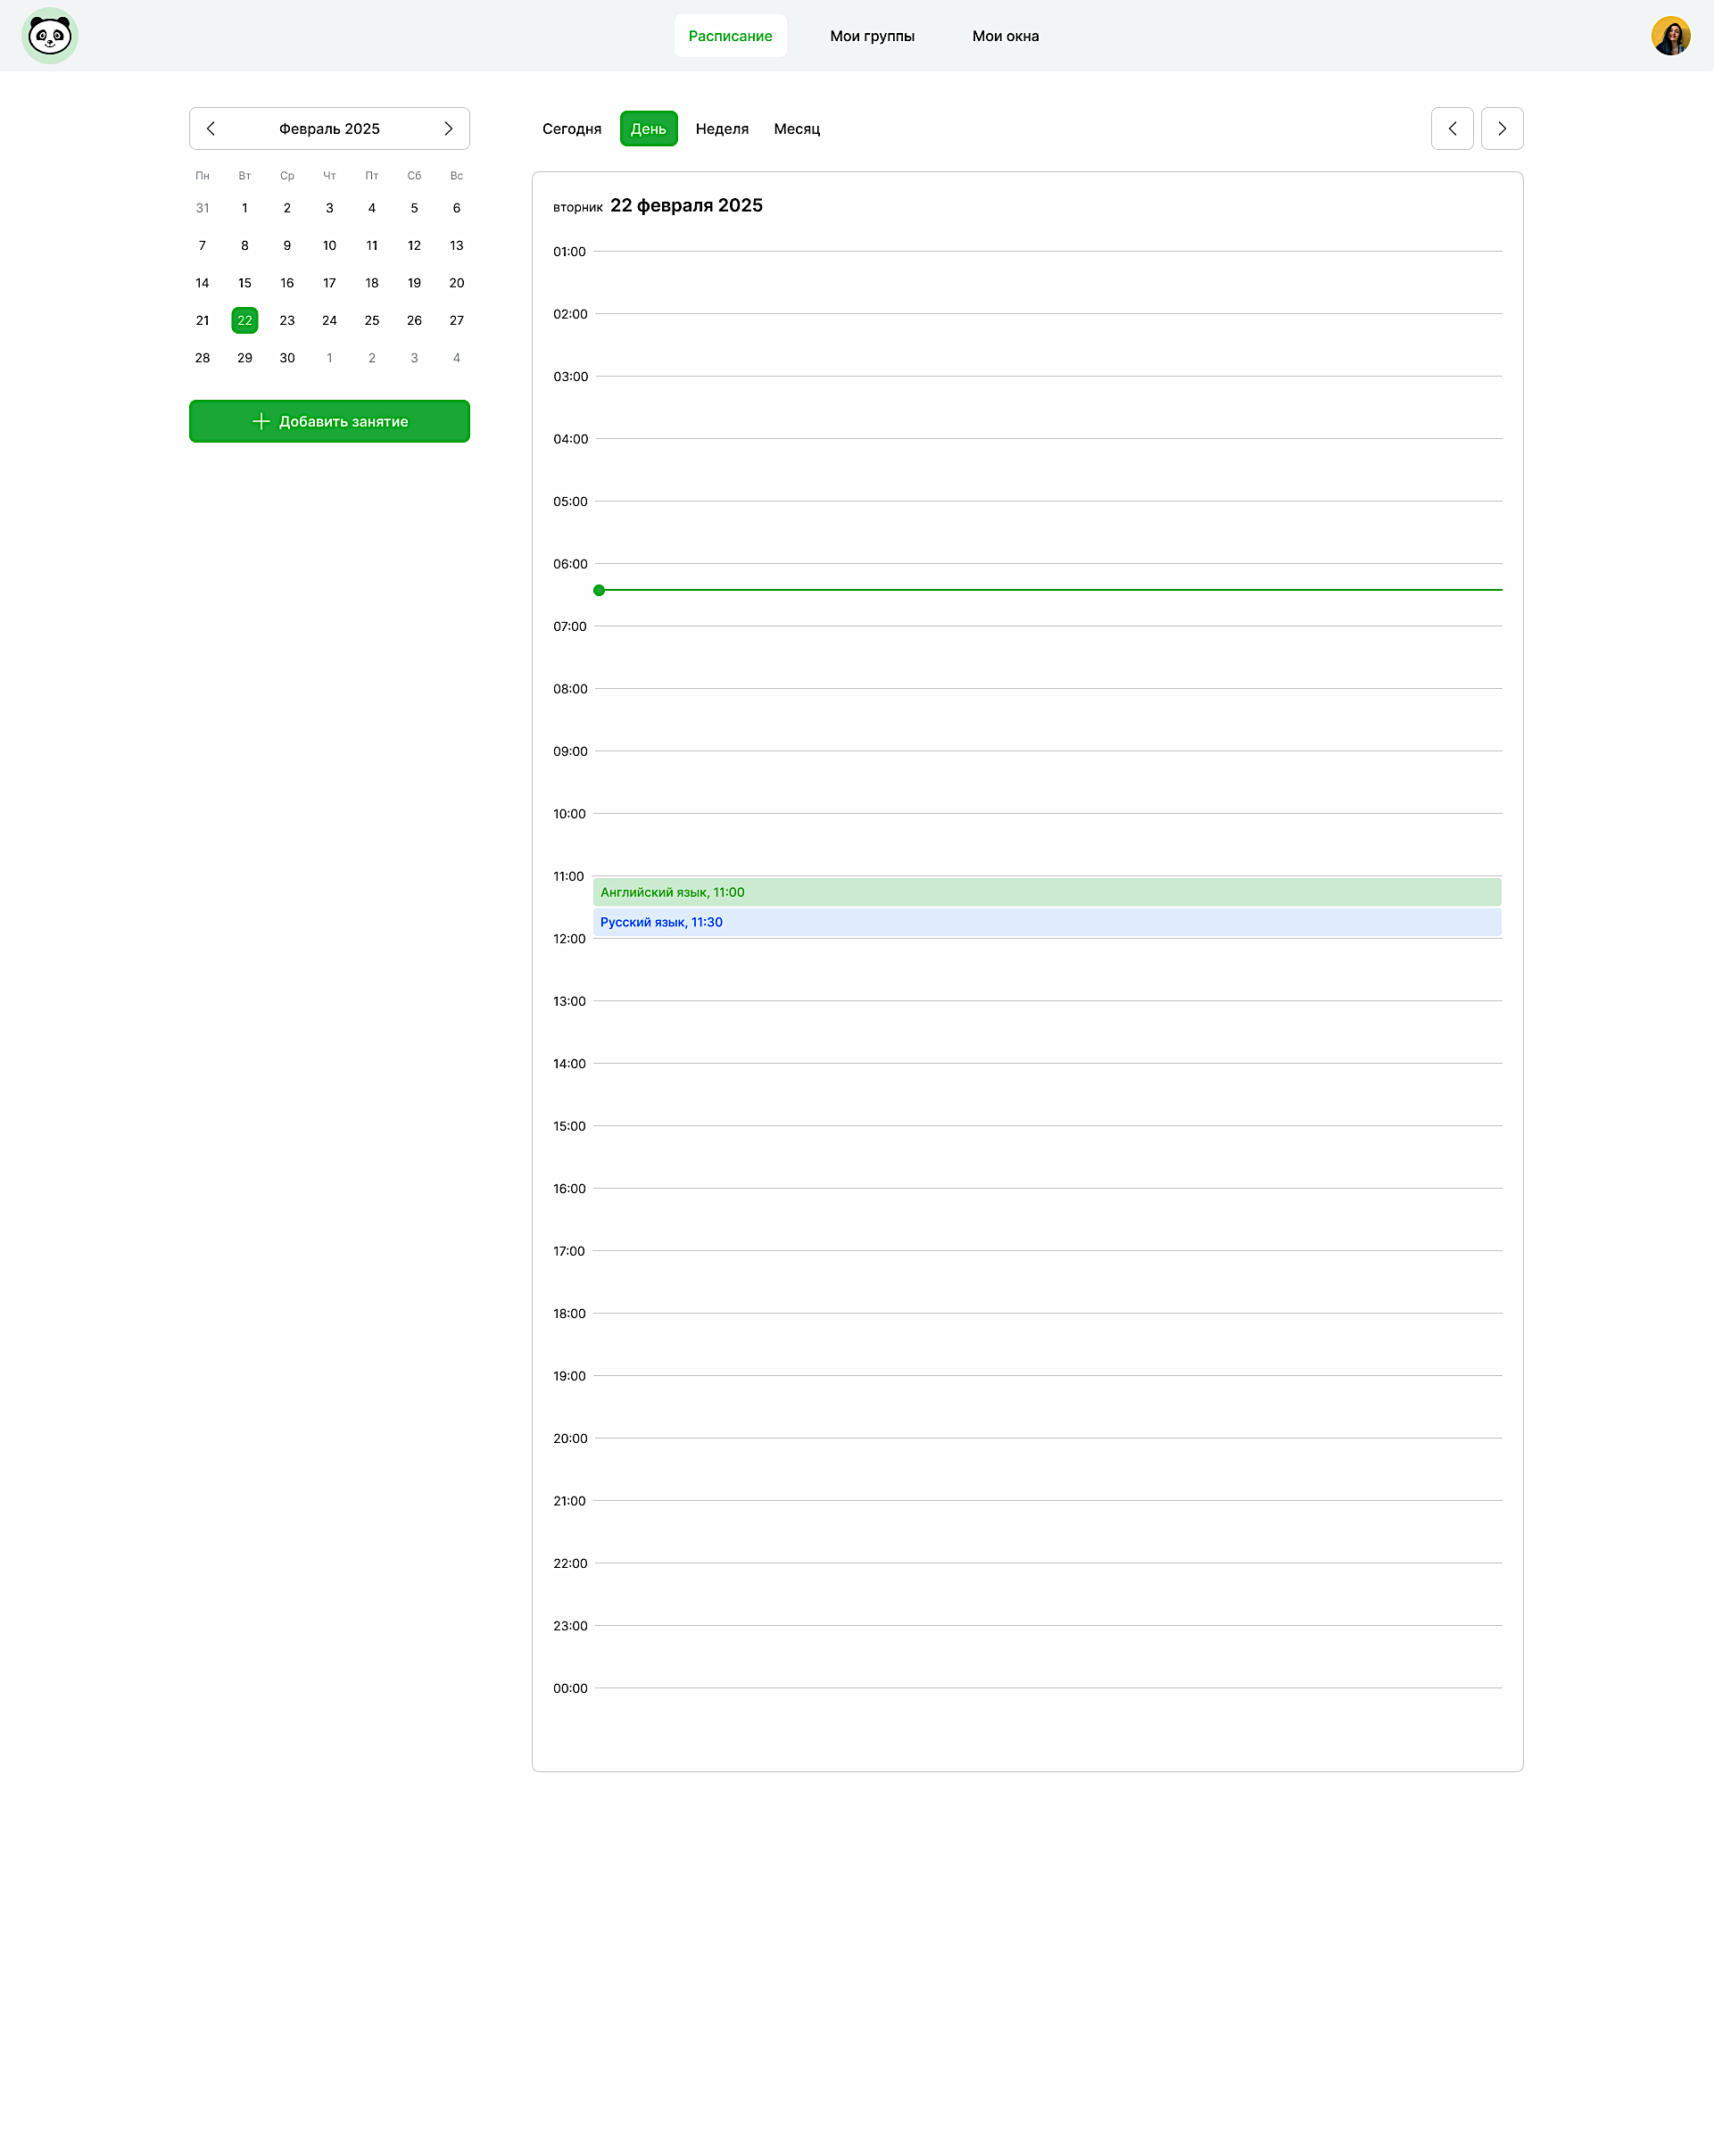
\includegraphics[width=1\linewidth]{images/design/Расписание_День.png}}
    % \captionof{figure}{Прототип страницы «Расписание». Календарь, день}

}

\section*{Б.3 Прототип страницы «Расписание». Календарь, неделя}


{
    \centering
    \fbox{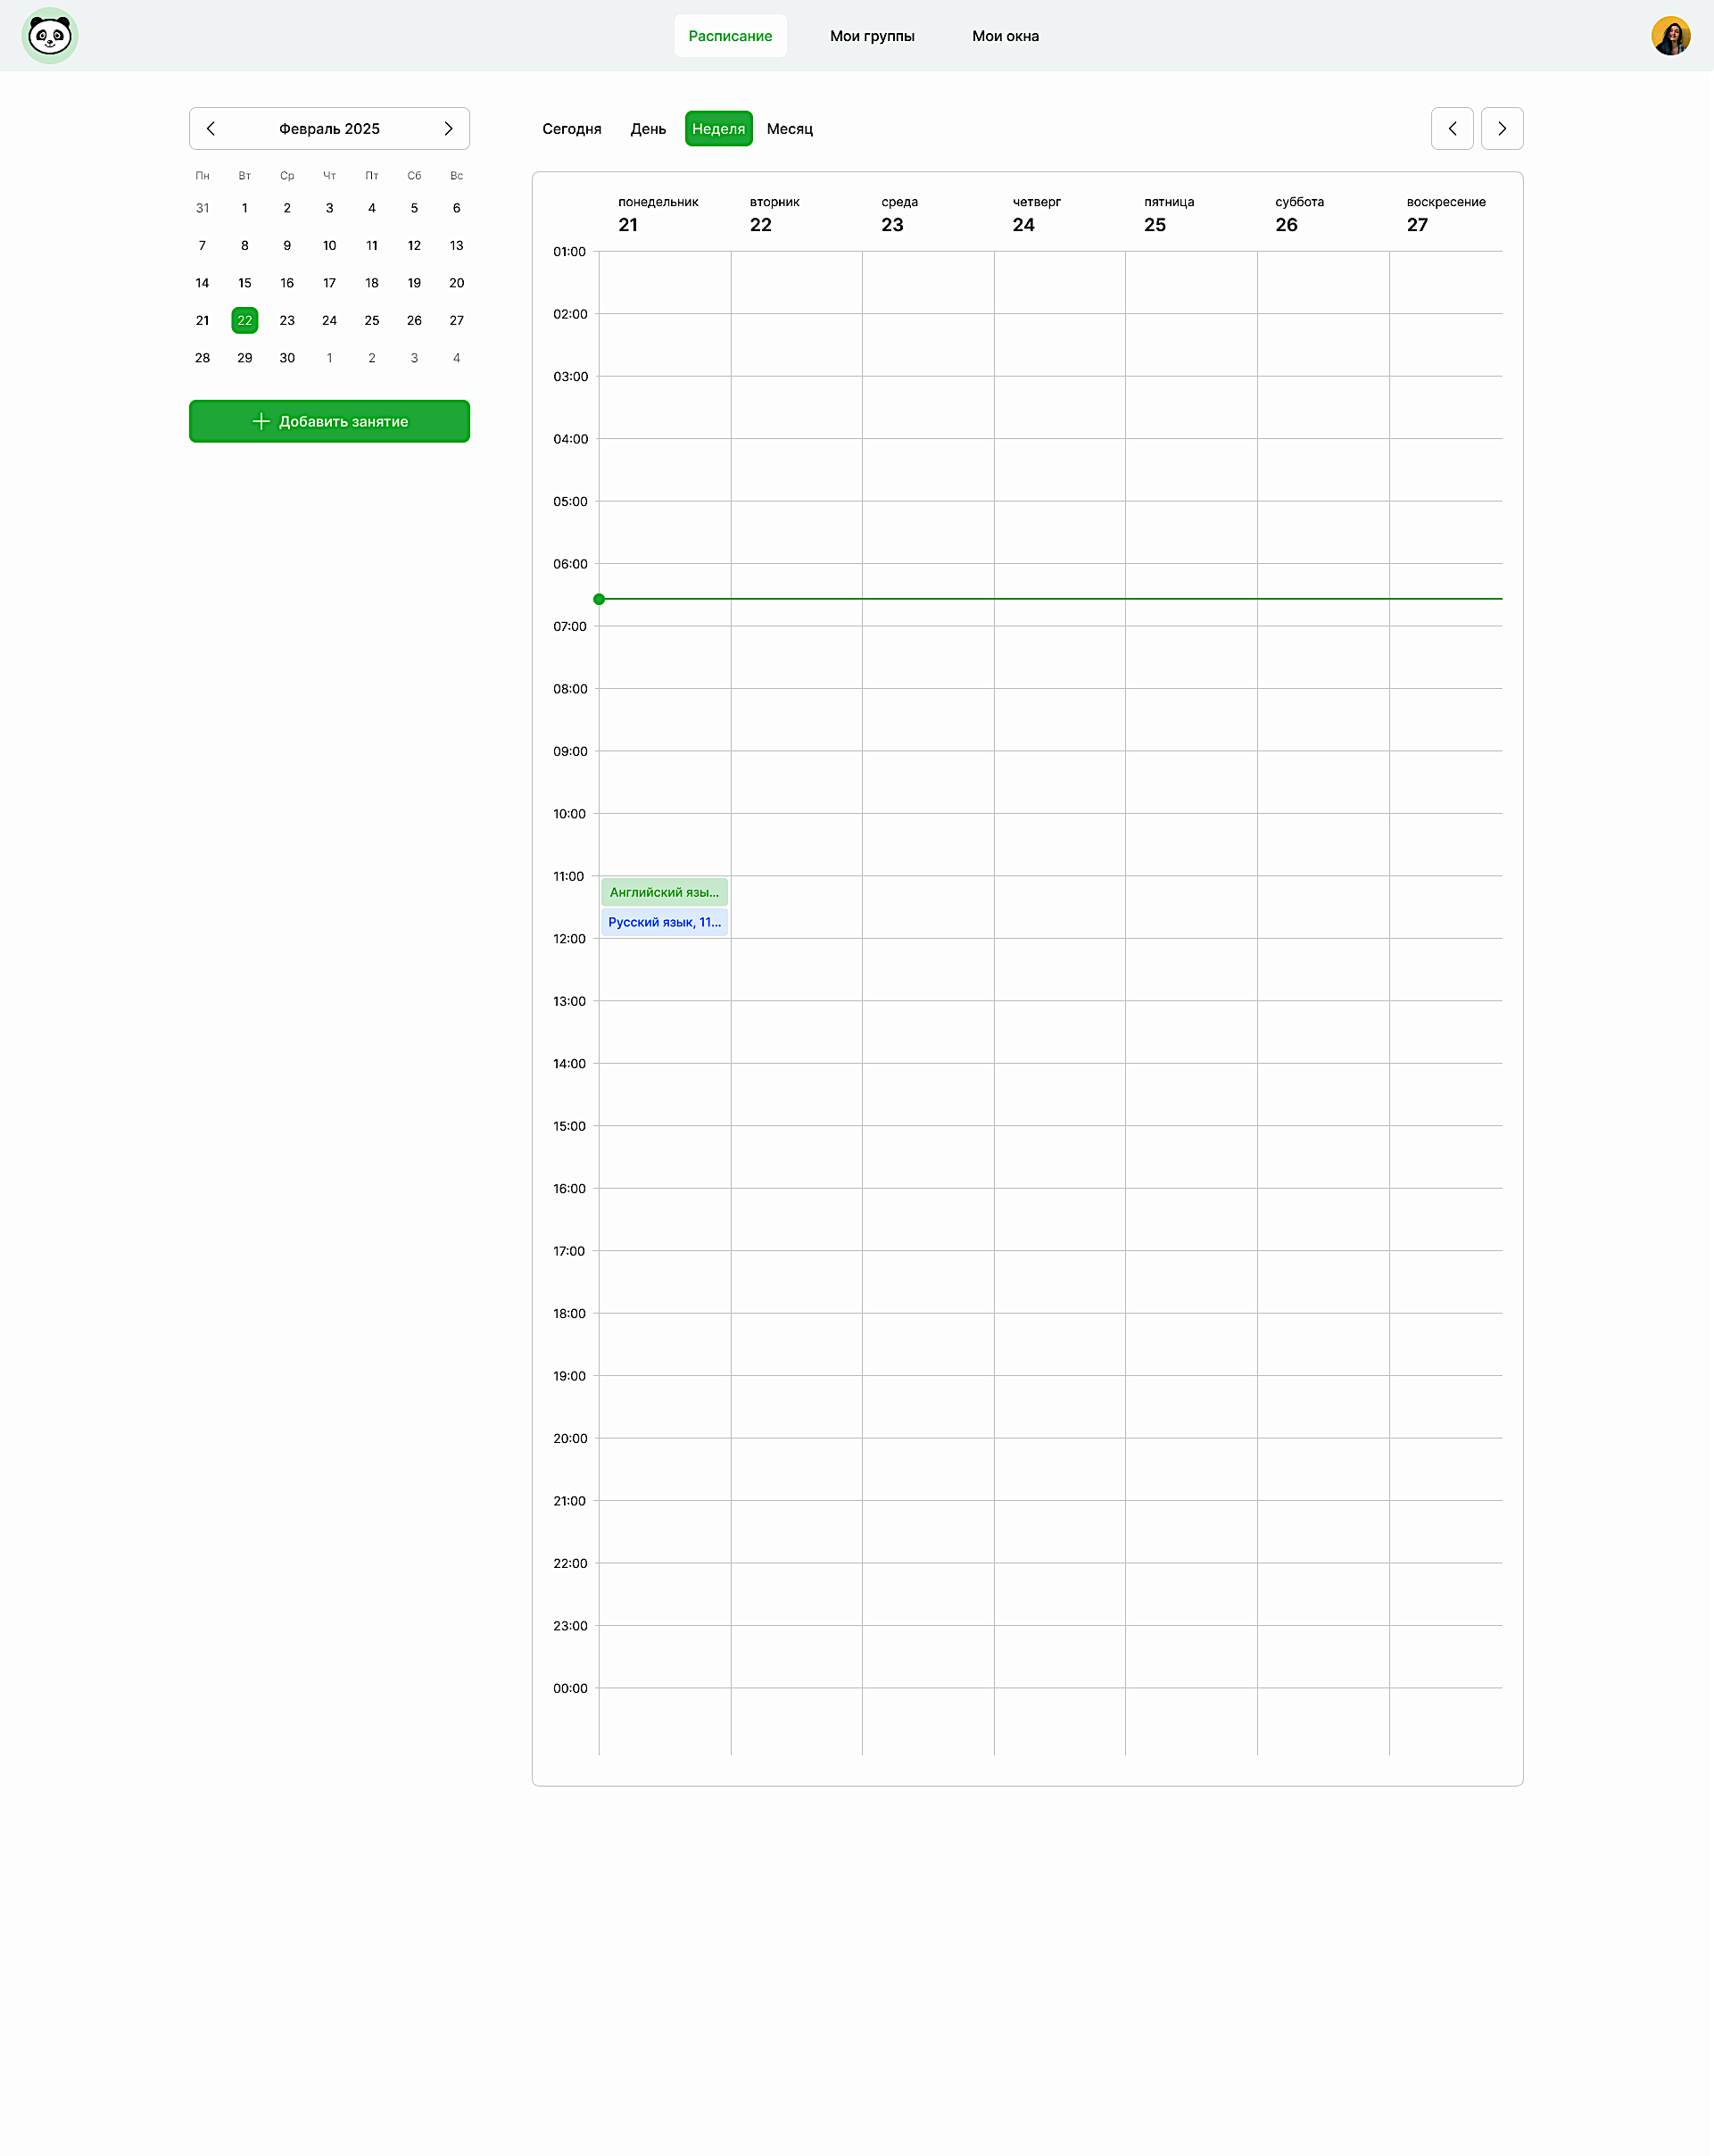
\includegraphics[width=1\linewidth]{images/design/Расписание_Неделя.png}}
    % \captionof{figure}{Прототип страницы «Расписание». Календарь, неделя}
}

\chapter*{ПРИЛОЖЕНИЕ В}


\addcontentsline{toc}{chapter}{ПРИЛОЖЕНИЕ В}
\setcounter{lstlisting}{0}
\renewcommand{\thelstlisting}{В.\arabic{lstlisting}}


\begin{lstlisting}[language=python, caption=Файл base.py с классом BaseCRUD,breaklines=true]
1 from sqlite3 import IntegrityError
2 import models as m
3 import api.exceptions as exc
4 from schemas import BaseListResponse
5 from functools import wraps
6 import typing as t
7 
8 
9 class BaseCRUD():
10     """BaseCRUD implements base common logic that can be used
11     by all other CRUD classes.
12 
13     Args:
14         db: SqlAlchemy Session instance
15         model: SqlAlchemy orm default model
16         joined_models: Optional list of models in which filters will work. Defaults to [model]
17     """
18 
19     def __init__(self, db, model, joined_models = []):
20         self.db = db
21         self.model = model
22         self.joined_models = [model] if len(joined_models) == 0 else joined_models
23 
24     def _save_to_db(self, item: t.Dict[str, t.Any]):
25         """Create new Item in db and return its new glory.
26 
27         Args:
28             item: children of BaseModel
29 
30         Returns:
31             created_item: children of BaseModel
32         """
33         self.db.add(item)
34         self.db.commit()
35         self.db.refresh(item)
36         return item
37     def get_item(self, body, field='id', model=None) -> m.BaseModel:
38         """Get one item from specific table by given field key and value.
39         Args:
40             value (schemas.RequestBodyOne) Request body
\end{lstlisting}
\noindent Продолжение листинга В.1
\vspace{13pt}
\begin{lstlisting}[language=python, breaklines=true, captionpos=none, title={}]
41         """
42         field (str): Field key of model of which type is searched.
43 
44         Returns:
45             Item in DB that was found in db.
46             None if provided field is not found on model.
47         """
48         model = self.model if model is None else model
49 
50         query = self.db.query(model)
51         if isinstance(field, str):
52             if not hasattr(model, field):
53                 raise exc.NotFoundError(message='No such field on model')
54             value = body.get(field)
55             if value is None:
56                 raise exc.NotFoundError(message='Value is null', field=field)
57             found_item = query.filter(getattr(model, field) == value).first()
58         elif isinstance(field, list):
59             for field_item in field:
60                 if not hasattr(model, field_item):
61                     raise exc.NotFoundError(message='No such field on model', field=field_item)
62                 value = body.get(field_item)
63                 if value is None: raise exc.NotFoundError(message='Value is null', field=field)
64                 query = query.filter(getattr(model, field_item) == value)
65             found_item = query.first()
66 
67 
68         if found_item and found_item.get('is_deleted', False):
69             raise exc.NotFoundError('Item is deleted')
70         else:
71             return found_item
72 
73     def get(self, body, field='id', model=None):
74         """Get one item from specific table by given field key and value.
75         Args:
76             value (schemas.RequestBodyOne) Request body
77             field (str): Field key of model of which type is searched.
78             Defaults to 'id'
79         Returns:
80             Item in DB that was found in db.
81             None if provided field is not found on model.
82         return self._make_output([self.get_item(body, field, model)])[0]
\end{lstlisting}
\noindent Продолжение листинга В.1
\vspace{13pt}
\begin{lstlisting}[language=python, breaklines=true, captionpos=none, title={}]
83     def _make_output(self, rows):
84         return rows
85 
86     def _transform_response(self, rows):
87         """Transform response into defined format.
88 
89         Args:
90             rows (list): List of items to wrap
91 
92         Returns:
93             schemas.BaseListResponse
94             .. code-block:: json
95             {
96                 "rows": [],
97                 "totalCount" : 0
98             }
99         """
100         rows = self._make_output(rows)
101         rows = [row.dict() if not isinstance(row, dict) else row for row in rows]
102         return BaseListResponse(rows=rows, totalCount=len(rows))
103 
104     def _transform_boolean(self, where):
105         if isinstance(where, dict) and where.get('value') and where.get('value') in ['false', 'true']:
106             where['value'] = where['value'].lower() in ("yes", "true", "t", "1")
107         return where
108     
109     def _get_column_from_joined_models(self, column_name):
110         for model in self.joined_models:
111             if hasattr(model, column_name):
112                 return getattr(model, column_name)
113             if column_name in model.__table__.columns:
114                 return model.__table__.columns[column_name]
115         raise ValueError(f"Column '{column_name}' not found in any of the provided models")
116     def list(self, body, model=None):
117         """Get one or multiple items in list representation:
118 
119         Args:
120             body(schemas.RequestBodyList)
121             .. code-block:: json
122             {
123                 "filters": {
124
\end{lstlisting}
\noindent Продолжение листинга В.1
\vspace{13pt}
\begin{lstlisting}[language=python, breaklines=true, captionpos=none, title={}]
125            """
126                    "wheres" : [
127                        {
128                            "column":column,
129                            "condition": condition,
130                            "value":value
131                        }
132                    ],
133                    "orders": [
134                        {
135                            "column": column,
136                            "desc": boolean
137                        }
138                    ],
139                    "search" : search value @todo,
140                    "page": integer @todo
141                    "limit": integer @todo
142                }
143            }
144            model (model): sqlalchemy model on which to perform queries.
145                Defaults to None, uses one in defined in constructor
146 
147        Returns:
148            response (schemas.BaseListResponse)
149        """
150        rows = self.get_items(body, model)
151        return self._transform_response(rows)
152 
153    def get_items(self, body, model=None):
154        model = self.model if model is None else model
155        filters = body.get('filters', {})
156 
157        wheres = filters.get('wheres', [])
158        orders = filters.get('orders', [])
159 
160        query = self.db.query(model)
161        if hasattr(model, 'is_deleted'):
162            query = query.filter(getattr(model, 'is_deleted') == False)
163        query, wheres = self._make_custom_query(query, wheres)
164        for where in wheres:
165            condition = where.get('condition')
166            where = self._transform_boolean(where)
167            column = self._get_column_from_joined_models(where['column'])
168            if condition == 'between':
169                query = query.filter(column.between(*where['value']))
170            elif condition == '!=':
\end{lstlisting}
\noindent Продолжение листинга В.1
\vspace{13pt}
\begin{lstlisting}[language=python, breaklines=true, captionpos=none, title={}]
171                query = query.filter(column != where['value'])
172            elif condition == 'in':
173                query = query.filter(column.in_(where['value']))
174            elif condition == '%':
175                query = query.filter(column.contains(where['value']))
176            else:
177                query = query.filter(column == where['value'])
178        for order in orders:
179            query = query.order_by(getattr(model, order['column']).desc(
180            ) if order['desc'] else getattr(model, order['column']).asc())
181 
182        print(query.statement.compile())
183         
184        return query.all()
185 
186    def _make_custom_query(self, query, wheres):
187        return query, wheres
188 
189    def _delete_item(self, body, field, model=None):
190        item_to_delete = self.get_item(body, field, model)
191        if not item_to_delete:
192            raise exc.NotFoundError(field=field)
193        self.db.delete(item_to_delete)
194        self.db.commit()
195        return item_to_delete
196 
197    def delete(self, body, field='id', model=None):
198        """Delete one item from specific table by given field
199 
200        Args:
201            body (RequestBodyOne or RequestBodyOnes) Request body
202            field (str): Field key of model of which type is searched. Defaults to 'id'
203            model (model): sqlalchemy model on which to perform queries.
204                Defaults to None, uses one in defined in constructor
205 
206        Returns:
207            Item in DB that was found in db.
208            None if provided field is not found on model.
209        """
210        model = self.model if model is None else model
211 
212        if not hasattr(model, field):
213            raise exc.NotFoundError(field=field)
214        if body.get('ids') and isinstance(body.get('ids'), list):
215            items_to_delete = []
\end{lstlisting}
\noindent Продолжение листинга В.1
\vspace{13pt}
\begin{lstlisting}[language=python, breaklines=true, captionpos=none, title={}]
216            for item in body.get('ids'):
217                item_to_delete = self._delete_item({'id': item}, field, model)
218                items_to_delete.append(item_to_delete)
219            return items_to_delete
220        else: return self._delete_item(body, field, model)
221 
222    def _is_value_empty(self, value) -> bool:
223        null_values = ['', 'null', 'None', b'']
224        return value in null_values
225 
226    def _is_immutable_field(self, field) -> bool:
227        immutable_fields = ['id', 'login']
228        return field in immutable_fields
229 
230    def update(self, body, model=None):
231        """Update one item from one specific table by given fields
232 
233        Args:
234            body (schemas.RequestBodyOne) Request body
235            model (model): sqlalchemy model on which to perform queries.
236                Defaults to None, uses one in defined in constructor
237 
238        Returns:
239            Item in DB that was found in db.
240        """
241        model = self.model if model is None else model
242        item_to_update = self.get_item(body, 'id', model)
243        if not item_to_update:
244            raise exc.NotFoundError()
245 
246        valid_values = {}
247 
248        body = body.dict() if hasattr(body, 'dict') else body
249 
250        for key, value in body.items():
251          if self._is_value_empty(value) or self._is_immutable_field(key):
252                continue
253            valid_values[key] = value
254 
255        self.db.query(model).filter(getattr(model, 'id') == 
256        item_to_update.get('id')).update(
257            valid_values
258        )
259 
260        self.db.commit()
\end{lstlisting}
\noindent Продолжение листинга В.1
\vspace{13pt}
\begin{lstlisting}[language=python, breaklines=true, captionpos=none, title={}]
261        self.db.refresh(item_to_update)
262 
263        return item_to_update
264    def mark_deleted(self, body, field='id', restore=False, model=None):
265        """Mark one item as deleted from specific table by given field key and value.
266 
267        Args:
268            value (schemas.RequestBodyOne) Request body
269            field (str): Field key of model of which type is searched. Defaults to 'id'
270            restore (bool): Flag by which item can be marked or restored. Defaults to False.as_integer_ratio
271            model (model): sqlalchemy model on which to perform queries.
272                Defaults to None, uses one in defined in constructor
273 
274        Returns:
275            Item in DB that was found in db.
276            None if provided field is not found on model.
277        """
278        model = self.model if model is None else model
279        if not hasattr(model, 'is_deleted'):
280            print(f'{model} do not have `is_deleted` property')
281            raise exc.InternalError()
282 
283        item_to_delete = self.get_item(body, field, model)
284        if not item_to_delete:
285            raise exc.NotFoundError(field=field)
286 
287        # setattr(item_to_delete, 'is_deleted', (not restore))
288        self.db.query(model).filter(getattr(model, field) == item_to_delete.get(
289            field)).update({'is_deleted': (not restore)})
290        self.db.commit()
291        self.db.refresh(item_to_delete)
292 
293        return item_to_delete
294 
295    def insert(self, request_body, model=None) -> dict:
296        model = self.model if model is None else model
297        if not isinstance(request_body, list):
298            request_body = [request_body]
299        inserted_items = [
300            model(
301                **{k: v for k, v in (item.items() if isinstance(item, dict) 
\end{lstlisting}
\noindent Окончание листинга В.1
\vspace{13pt}
\begin{lstlisting}[language=python, breaklines=true, captionpos=none, title={}]
302                    else item.model_dump().items()) if k in model.__table__.columns
303        ]
304                }
305            ) for item in request_body
306        created_items = []
307        for item in inserted_items:
308            created_items.append(self._save_to_db(item))
309        return created_items

\end{lstlisting}

\begin{lstlisting}[language=python, caption=Файл auth.py с классом Authorisation,breaklines=true]
1 """
2 Logic to work with DB
3 """
4 from datetime import datetime, timedelta, timezone
5 from sqlalchemy.orm import Session
6 from sqlalchemy import and_
7 import models as m
8 from schemas import UserCreate, UserLogin, UserOut, Token
9 from fastapi import Depends
10 from fastapi.security import OAuth2PasswordBearer
11 from crud.base import BaseCRUD
12 import api.exceptions as exc
13 from database import get_db
14 from jose import JWTError, jwt
15 from env_constants import SECRET_KEY, ACCESS_TOKEN_EXPIRE_MINUTES, BASE_URL
16 import typing as t
17 
18 import bcrypt
19 
20 oauth2_scheme = OAuth2PasswordBearer(
21     tokenUrl=f'/{BASE_URL}/auth/login', auto_error=False)
22 ALGORITHM = 'HS256'
23 
24 
25 async def authorised_user(token: str = Depends(oauth2_scheme), db: Session = Depends(get_db)) -> UserOut:
26     """Dependency by which access is guaranteed only to authorised users.
27     Token should be placed in Authoruisation Header of any request that requires authorised access.
28 
29     Example of Header placement:`Authorization:'Bearer<your JWT token>'`
30     Args:
    \end{lstlisting}
    \noindent Продолжение листинга В.2
    \vspace{13pt}
    \begin{lstlisting}[language=python, breaklines=true, captionpos=none, title={}]
31     """
32         `token` (str): JWT access token from headers
33     Returns:
34         Authorised user
35     Raises:
36         AuthorisationError: If provided token is mismatched
37         does not exist
38     """
39     if Authorisation(db)._is_token_revoked(token):
40         raise exc.AuthorisationError('Token is expired. Log in again')
41     try:
42         payload = jwt.decode(token, SECRET_KEY, algorithms=[ALGORITHM])
43         username = payload.get('sub')
44         if username is None:
45             raise exc.AuthorisationError('Could not validate credentials')
46     except (JWTError, AttributeError):
47         raise exc.AuthorisationError('Provided token is invalid')
48     user = Authorisation(db)._get_user_by_login(username)
49     if user is None:
50         raise exc.AuthorisationError('Could not validate credentials')
51     return user
52 
53 
54 class Authorisation(BaseCRUD):
55     def __init__(self, db: Session):
56         super().__init__(db, m.User)
57 
58     def register(self, body: UserCreate) -> UserOut:
59         """Register user.
60 
61         Args:
62             `body` (UserCreate): User data for creation
63 
64         Returns:
65             New registered user
66 
67         Raises:
68         """
69             exc.ValidationError
70         """
71         login = body.get('login')
72         existing_user = self._get_user_by_login(login)
73         if (existing_user):
74             raise exc.ValidationEror(
75                 message='Username already registered', field='login')
76         password = body.get('password')
\end{lstlisting}
\noindent Продолжение листинга В.2
\vspace{13pt}
\begin{lstlisting}[language=python, breaklines=true, captionpos=none, title={}]
77         password_confirm = body.get('password_confirm')
78         if (password != password_confirm):
79             raise exc.ValidationEror(
80                message='Passwords do not match', field='password_confirm')
81         hashed_password = self._hash_password(password)
82 
83         new_body = body
84         new_body.password = hashed_password
85         return super().insert(new_body)[0]
86 
87     def _hash_password(self, password: t.Optional[str]) -> str:
88         """Hash password with bcrypt module.
89 
90         Args:
91             password (str): plain password from request.
92 
93         Returns:
94             hashed_password (str): hashed password.
95         """
96         if password is None:
97             return ''
98         return bcrypt.hashpw(password.encode('utf-8'), bcrypt.gensalt()).decode('utf-8')
99 
100    def login(self, auth_creds: UserLogin) -> Token:
101        """Authorise user. Create JWT token for future access.
102 
103        Args:
104            `auth_creds` (UserLogin): Credentials for authorisation
105 
106        Returns:
107            Token for future access
108 
109        Raises:
110            ValidationEror if db does not have user with provided login
111        """
112        user = self._verify_token(
113            auth_creds.get('login'), auth_creds.get('password')
114        )
115        if not user:
116            raise exc.ValidationEror(field=['login', 'password'])
117 
118        access_token_expires = timedelta(minutes=ACCESS_TOKEN_EXPIRE_MINUTES)
119        access_token = self._create_access_token(
120            data={'sub': user.login}, expires_delta=access_token_expires
\end{lstlisting}
\noindent Продолжение листинга В.2
\vspace{13pt}
\begin{lstlisting}[language=python, breaklines=true, captionpos=none, title={}]
121        )
122        return {'access_token': access_token, 'token_type': 'bearer',
123        'user_id': user.get('id')}
124    def _verify_token(self, username: str, password: str) -> t.Union[UserOut, bool]:
125        """Verify if user exists and given password match one in db.
126 
127        Args:
128            `username` (str): login for auth.
129            `password` (str): plain password for auth check.
130 
131        Returns:
132            False if there is no such user or passwords do not match. \n
133            User if one exists.
134        """
135        user = self._get_user_by_login(username)
136        if not user or not self._verify_password(password, user.get('password')):
137            return False
138        return user
139 
140    def _verify_password(self, plain_password: str, hashed_password: str) -> bool:
141        """Verify plain password's hash matches one in db.
142 
143        Args:
144            plain_password (str): plain password from request
145            hashed_password (str): hash of plain password stored in db
146 
147        Returns:
148            bool Result of match
149        """
150        return bcrypt.checkpw(plain_password.encode('utf-8'), hashed_password.encode('utf-8'))
151    def _get_user_by_login(self, login: str) -> t.Optional[t.Union[UserOut, None]]:
152        """Get user by login.
153 
154        Args:
155            login (str): Login by which search will be run.
156 
157        Returns:
158            m.User if one exists with provided login else None.
159        """
160        return self.db.query(m.User).where(
161            and_(m.User.login==login, m.User.is_deleted == False)).first()
\end{lstlisting}
\noindent Окончание листинга В.2
\vspace{13pt}
\begin{lstlisting}[language=python, breaklines=true, captionpos=none, title={}]    
162    def _create_access_token(self, data, expires_delta: timedelta):
163        """Create and encode JWT token for future access.
164        Args:
165 
166            data: login by which jwt check authorisation.
167            expires_delta: duration of time by which token is valid.
168        Returns:
169            Encoded JWT token
170        """
171        to_encode = data.copy()
172        if expires_delta:
173            expire = datetime.now(timezone.utc) + expires_delta
174        else:
175            expire = datetime.now(timezone.utc) + timedelta(minutes=15)
176        to_encode.update({"exp": expire})
177        encoded_jwt = jwt.encode(to_encode, SECRET_KEY, algorithm=ALGORITHM)
178        return encoded_jwt
179 
180    def logout(self, token: Token) -> dict:
181        """Logout from current session
182        Args:
183            token (Token): Token to be resttricted
184        """
185        revoked_token = m.RevokedToken(token=token.access_token)
186        self.db.add(revoked_token)
187        self.db.commit()
188        return {"message": "Successfully logged out"}
189 
190    def _is_token_revoked(self, access_token: str) -> bool:
191        """Checks if token is revoked.
192        Args:
193        """
194            access_token (str): Token access_token
195        Returns:
196            bool if token is revoked or not
197        """
198        return self.db.query(m.RevokedToken).filter(m.RevokedToken.token == access_token).first() is not None
\end{lstlisting}

\begin{lstlisting}[language=JavaScript, caption=Генерация маршрутов внутри приложения,breaklines=true]
1 const generateRoutes = sections => {
2     const routes = []
3     sections.forEach(section => {
4         const defaultComponentName = `${capitalize(section.name)}Page`
\end{lstlisting}
\noindent Продолжение листинга В.3
\vspace{13pt}
\begin{lstlisting}[language=JavaScript, breaklines=true, captionpos=none, title={}]
5         const defaultComponent = 
6         importComponent(`${section.name}/${defaultComponentName}`)
7 
8         if (!section?.actions?.length) {
9             routes.push({
10                 path: `/${section.name}`,
11                 name: `${section.name}`,
12                 component: defaultComponent,
13             })
14         } else {
15             section.actions.forEach(action => {
16                 const component = importComponent(
17                     `${section.name}/${capitalize(section.name)}${capitalize(action)}Page`
18                 )
19                 console.log(`${section.name}/${capitalize(section.name)}${capitalize(action)}Page`)
20                 let pathAction = `/:action(${action})`
21                 const path =
22                     section.useId && !['list', 'new'].includes(action)
23                         ? `/${section.name}/${pathAction}/:id`
24                         : `/${section.name}/${pathAction}`
25                 routes.push({
26                     path,
27                     name: `${section.name}-${action}`,
28                     component,
29                 })
30             })
31         }
32     })
33     return routes
34 }
\end{lstlisting}
\begin{lstlisting}[language=JavaScript, caption=Процесс инициализации авторизации YandexOauth,breaklines=true, ]
1 async initYandexAuth() {
2     /* eslint-disable no-undef */
3     await this.loadBtnScript(
4         'https://yastatic.net/s3/passport-sdk/autofill/v1/sdk-suggest-with-polyfills-latest.js'
5     )
6     try {
7         const { handler } = await YaAuthSuggest.init(
8             /* eslint-enable no-undef */
9             {
10                 client_id: YANDEX_CLIENT_ID,
\end{lstlisting}
\noindent Продолжение листинга В.4
\vspace{13pt}
\begin{lstlisting}[language=JavaScript, breaklines=true, captionpos=none, title={}]
11                 response_type: 'token',
12                 redirect_uri: `http://${window.location.hostname}:1024/auth/
13                 yandex-callback`,
14                 display: 'page',
15             },
16             null,
17             {
18                 display: 'page',
19                 view: 'button',
20                 parentId: 'auth-bottom',
21                 buttonView: 'main',
22                 buttonTheme: 'light',
23                 buttonSize: 'm',
24                 buttonBorderRadius: 8,
25             }
26         )
27         await handler()
28     } catch (error) {
29         console.error('Yandex auth error:', error)
30     }
31 },
32 created() {
33 this.initYandexAuth()
\end{lstlisting}
\begin{lstlisting}[language=JavaScript, caption=Процесс авторизации через Google,breaklines=true, ]
1 async initGoogleAuth() {  
2     await this.loadBtnScript('https://accounts.google.com/gsi/client?hl=ru')  
3     try {  
4         /* eslint-disable no-undef */  
5         await google.accounts.id.initialize({  
6             client_id: GOOGLE_CLIENT_ID,  
7             callback: ({ credential }) => {  
8                 const userData = jwtDecode(credential)  
9                 const password = this.transformPassword(  
10                    `${userData.sub}-${userData.email.ucFirst()}`  
11                )  
12                this.$api.auth.register(  
13                    {  
14                        name: userData.given_name,  
15                    },  
16                    () => {  
17                        this.authorize({  
18                            login: userData.email,  
\end{lstlisting}
\noindent Продолжение листинга В.5
\vspace{13pt}
\begin{lstlisting}[language=JavaScript, breaklines=true, captionpos=none, title={}]
19                             password: password,  
20                         })  
21                     }  
22                 )  
23             },  
24             response_type: 'token',  
25             scope: 'https://www.googleapis.com/auth/userinfo.profile https://www.googleapis.com/auth/userinfo.email openid',  
26             ux_mode: 'popup',  
27         })  
28         google.accounts.id.renderButton(document.getElementById('auth-bottom2'), {  
29             theme: 'outline',  
30             size: 'large',  
31             locale: 'ru',  
32         })  
33         google.accounts.id.prompt() // also display the One Tap dialog  
34         /* eslint-enable no-undef */  
35     } catch (error) {  
36         console.error('Google auth error:', error)  
37     }  
38 },  
39  
40 created() {  
41     // other code  
42     this.initGoogleAuth()  
43     // other code  
44 }  
\end{lstlisting}

\end{document}
